\chapter{Analysis of the Higgs boson at the LHC} \label{chap:chap-4}


% \begin{singlespace}
%     \epigraph{This is a large quote placed with \\ 
%     single spacing over two lines}{-- Unknown Author}
% \end{singlespace}


%% remove the following and add your chapter text here
% \section{A long section heading to test the distance before this}

% \blindtext

% \begin{figure}[ht]
% \begin{center}
%     \includegraphics[width=\textwidth, trim={6cm 5cm 6cm 5cm},clip,page=1] {chap4.pdf}
%     \caption{Here are some photos of ducks to make you feel happy in tough times.}
%     \label{fig:ducks}
% \end{center}
% \end{figure}

% \Blindtext[2]





% The SM postulates the existence of a Higgs field responsible for generating the masses of fundamental particles. The quantum excitation of this field is known as the Higgs boson ($H$)~\cite{StandardModel67_1, Englert:1964et, Higgs:1964ia, Higgs:1964pj, Guralnik:1964eu, StandardModel67_2, StandardModel67_3}. The properties of the \Hboson, observed with a mass of approximately 125\,GeV by the ATLAS and CMS Collaborations~\cite{Aad:2012tfa, Chatrchyan:2012xdj, Chatrchyan:2013lba} at the LHC, have been found to be consistent with the expectations of the SM~\cite{ATLASnature, CMSnature}. The mass of the \Hboson ($m_{H}$) is a free parameter of the model and, since it determines all other Higgs properties, should be measured with the highest possible precision. For instance, the Higgs boson’s couplings to vector bosons strongly depend on $m_H$ and are precisely predicted within the SM.

% Another critical property of the \Hboson is its lifetime, which is predicted in the SM to be $1.6\times10^{-22}$\,s, corresponding to a total width ($\Gamma_H$) of 4.1\,MeV~\cite{deFlorian:2016spz}, assuming $m_H = 125$\,GeV. Any deviation from this prediction would suggest the presence of anomalous Higgs couplings or decays into previously undetected particles. Hence, a precision measurement of the width ($\Gamma_H$) is valuable in the search for BSM physics. 

% The ATLAS and CMS Collaborations initially measured the \Hboson mass to be $125.09 \pm 0.24$\,GeV~\cite{Aad:2015zhl}, using $\sqrt{s} = 7$ and 8\,TeV proton-proton (pp) collision data from the 2011–2012 data-taking period (Run~1), corresponding to a total integrated luminosity of 25\,fb$^{-1}$ per experiment. This result has since been superseded by both experiments. The ATLAS Collaboration measured the \Hboson mass to be $125.11 \pm 0.11$\,GeV~\cite{ATLAS_mass}, combining the $H \to \gamma\gamma$ and $H \to 4\ell$ ($\ell = e$, $\mu$) channels from Run~1 and data collected at $\sqrt{s} = 13$\,TeV during 2015–2018 (Run~2). The value in parentheses indicates the statistical uncertainty only. The most recent CMS measurement, also using the $H \to \gamma\gamma$ and $H \to 4\ell$ channels and including Run~1 data together with 36\,fb$^{-1}$ of $\sqrt{s} = 13$\,TeV data from 2016, yields $m_{H} = 125.38 \pm 0.14$\,GeV, with a statistical uncertainty of 0.11\,GeV. Independent measurements using only the $H \to 4\ell$ channel and 2016 data report $m_H = 124.94 \pm 0.18$\,GeV (ATLAS) and $125.26 \pm 0.21$\,GeV (CMS), with statistical uncertainties of 0.17\,GeV and 0.19\,GeV, respectively.

% Assuming only on-shell Higgs boson production, CMS has set an upper limit on the \Hboson width of $\Gamma_H < 1.10$\,GeV at 95\% confidence level (CL), constrained by the four-lepton invariant mass resolution~\cite{Khachatryan:2014jba, Sirunyan:2017exp}. Both ATLAS and CMS have also constrained $\Gamma_H$~\cite{Khachatryan:2014iha, Aad:2015xua, Khachatryan:2015mma, Khachatryan:2016ctc, Aaboud:2018puo, Sirunyan:2019twz, CMS:2022ley} using an off-shell production method~\cite{Caola:2013yja, Kauer:2012hd, Campbell:2013una}, which relies on the measurement of the ratio of off-shell to on-shell production rates. Taking into account both gluon fusion (ggH) and electroweak (EW) production processes, the most recent results are $\Gamma_H = 3.2^{+2.4}_{-1.7}$\,MeV~\cite{CMS:2022ley} and $\Gamma_H = 4.3^{+3.3}_{-2.5}$\,MeV~\cite{atlascollaboration2023evidence}, reported by CMS and ATLAS, respectively. Furthermore, CMS has set a lower bound of $\Gamma_H > 3.5\times10^{-9}$\,MeV at 95\% CL, based on limits on the \Hboson flight distance in the detector~\cite{Khachatryan:2015mma}.

% In this chapter, I present an updated CMS measurement of the \Hboson width using off-shell production in the $H^* \to 4\ell$ decay channel. Additionally, I include results from a Higgs boson mass measurement conducted by collaborators using the shared on-shell data sample. The analysis is based on 138\,fb$^{-1}$ of $pp$ collision data at $\sqrt{s} = 13$\,TeV, collected from Run~2 between 2016 and 2018, combined with Run~1 data.

As previously discussed in Section~\ref{sec:higgs}, the SM postulates the existence of a scalar field---the Higgs field---responsible for the generation of mass for fundamental particles through the mechanism of electroweak symmetry breaking. The excitation of this field is known as the Higgs boson ($H$)~\cite{StandardModel67_1, Englert:1964et, Higgs:1964ia, Higgs:1964pj, Guralnik:1964eu, StandardModel67_2, StandardModel67_3}. The properties of the Higgs boson, observed with a mass of approximately 125\,GeV by the ATLAS and CMS Collaborations~\cite{Aad:2012tfa, Chatrchyan:2012xdj, Chatrchyan:2013lba} at the Large Hadron Collider (LHC), are found to be in agreement with SM predictions~\cite{ATLASnature, CMSnature}. 

The mass of the Higgs boson ($m_H$) is a free parameter in the SM and governs all other Higgs properties, necessitating its measurement with the highest possible precision. For instance, the Higgs boson couplings to vector bosons depend strongly on $m_H$ and are predicted with high precision within the SM framework. Another key parameter is the Higgs boson's total decay width ($\Gamma_H$), which determines its lifetime. The SM predicts a width of $\Gamma_H = 4.1$\,MeV, corresponding to a lifetime of $1.6 \times 10^{-22}$\,s~\cite{deFlorian:2016spz} for $m_H = 125$\,GeV. Any deviation from this prediction could signal anomalous Higgs couplings or decays to invisible or non-SM particles.

Using $\sqrt{s} = $7 and 8\,TeV proton-proton (pp) collision data collected during Run~1 (2011–2012), the ATLAS and CMS Collaborations jointly measured the Higgs boson mass as $125.09 \pm 0.24$\,GeV~\cite{Aad:2015zhl}, based on a combined integrated luminosity of 25\,fb$^{-1}$ per experiment. This result has since been superseded. The ATLAS Collaboration, combining the $H \to \gamma\gamma$ and $H \to 4\ell$ ($\ell = e, \mu$) decay channels using both Run~1 and Run~2 ($\sqrt{s} = 13$\,TeV, 2015–2018) data, reported a measurement of $m_H = 125.11 \pm 0.11\,\mathrm{GeV}$, with a statistical uncertainty of 0.09\,GeV~\cite{ATLAS_mass}. The most recent CMS result, using the same decay channels and including Run~1 and 36\,fb$^{-1}$ of 2016 data, yields $m_H = 125.38 \pm 0.14\,\mathrm{GeV}$, with a statistical uncertainty of 0.11\,GeV. Independent measurements from ATLAS and CMS based solely on the $H \to 4\ell$ decay and 2016 data give $m_H = 124.94 \pm 0.18 (\pm 0.17)$\,GeV and $m_H = 125.26 \pm 0.21 (\pm 0.19)$\,GeV, respectively, where the value in parentheses is the statistical uncertainty only.

Assuming only on-shell production, CMS placed an upper limit on the Higgs boson width of $\Gamma_H < 1.10$\,GeV at 95\% confidence level (CL), constrained by the four-lepton invariant mass resolution~\cite{Khachatryan:2014jba, Sirunyan:2017exp}. Both ATLAS and CMS have also set more stringent constraints using the off-shell production method~\cite{Khachatryan:2014iha, Aad:2015xua, Khachatryan:2015mma, Khachatryan:2016ctc, Aaboud:2018puo, Sirunyan:2019twz, CMS:2022ley}, which exploits the ratio of off-shell to on-shell production cross sections~\cite{Caola:2013yja, Kauer:2012hd, Campbell:2013una}. This method yields recent measurements of $\Gamma_H = 3.2^{+2.4}_{-1.7}$\,MeV by CMS~\cite{CMS:2022ley}, and $\Gamma_H = 4.3^{+3.3}_{-2.5}$\,MeV by ATLAS~\cite{atlascollaboration2023evidence}. Additionally, from limits on the Higgs flight distance in the detector, CMS set a lower bound of $\Gamma_H > 3.5 \times 10^{-9}$\,MeV at 95\% CL~\cite{Khachatryan:2015mma}.

In this chapter, I present an updated CMS measurement of the \Hboson width using off-shell production in the $H^* \to 4\ell$ decay channel. Additionally, I include results from an extension of the off-shell analysis, as well as a Higgs boson mass measurement conducted by collaborators using the shared on-shell data sample. The analysis is based on 138\,fb$^{-1}$ of $pp$ collision data at $\sqrt{s} = 13$\,TeV, collected from Run~2 between 2016 and 2018, combined with Run~1 data.

% This thesis presents an updated CMS measurement of the Higgs boson width using off-shell production in the $H^* \to 4\ell$ decay channel. It also includes a mass measurement performed by collaborators using the same on-shell dataset. The analysis is based on a combined dataset of 138\,fb$^{-1}$ of $pp$ collision data at $\sqrt{s} = 13$\,TeV collected from 2016 to 2018, along with data from Run~1.







% The SM of particle physics postulates the existence of a Higgs field responsible for the
% generation of the masses of fundamental particles. The excitation of this
% field is known as the Higgs boson ($H$)~\cite{StandardModel67_1, Englert:1964et,Higgs:1964ia,
% Higgs:1964pj,Guralnik:1964eu,StandardModel67_2,StandardModel67_3}.
% The properties of the \Hboson, observed with a mass of approximately 125 GeV by the ATLAS and CMS
% Collaborations~\cite{Aad:2012tfa,Chatrchyan:2012xdj,Chatrchyan:2013lba} at the LHC, are found to be consistent with
% the expectations of the SM~\cite{ATLASnature,CMSnature}. The mass of the \Hboson ($m_{H}$) is a free parameter of the model and, since it determines all other Higgs properties, should be measured with as high precision as possible.
% For example, the Higgs boson couplings to vector bosons strongly depend on the \Hboson mass and are precisely predicted by the SM.
% Another important \Hboson characteristic is its lifetime, predicted by the SM to be $1.6\times10^{-22}$\,s, corresponding to a total width ($\Gamma_H$) of $4.1$ MeV~\cite{deFlorian:2016spz},
% as predicted precisely within the SM for $m_{H} = 125$ GeV.
% A deviation from the SM prediction would point to either anomalous \Hboson couplings or its decay to yet undiscovered particles.

% The ATLAS and CMS Collaborations measured the \Hboson mass to be $125.09 \pm 0.24$ GeV~\cite{Aad:2015zhl} using $\sqrt{s}=7$ and 8 TeV proton-proton (pp) collision data from the 2011--2012 data-taking periods (Run1), corresponding to a total integrated luminosity per experiment of 25 $fb^{-1}$.
% This result has been superseded by both collaborations.
% The ATLAS experiment measured the \Hboson mass to be $125.11 \pm 0.11 (\pm 0.09)$ GeV~\cite{ATLAS_mass}, combining the $H \to \gamma\gamma$ and $H \to 4\ell$ ($\ell = e$, $\mu$) channels from Run 1 and data collected at $\sqrt{s}=13$ TeV in 2015--2018 (Run~2).
% The value in parentheses is the statistical uncertainty only.
% The most recent CMS result, also using the $H \to \gamma\gamma$ and $H \to 4\ell$ channels and including Run 1 and 36 $fb^{-1}$ of $\sqrt{s}=13$ TeV data from 2016, is 
% $m_{H}$ = $125.38 \pm 0.14$ $(\pm 0.11)$ GeV.
% Measurements from ATLAS and CMS using only the $H \to 4\ell$ channel and 2016 data are $124.94 \pm 0.18 (\pm 0.17)$ GeV and $125.26 \pm 0.21 (\pm 0.19)$ GeV, respectively.

% Considering only on-shell Higgs boson production, CMS set an upper limit 
% on the \Hboson width $\Gamma_H < 1.10$ GeV at 95\% confidence level (CL), 
% limited by the four-lepton invariant mass resolution~\cite{Khachatryan:2014jba,Sirunyan:2017exp}.
% Both the ATLAS and CMS experiments have also set limits on 
% $\Gamma_H$~\cite{Khachatryan:2014iha,Aad:2015xua,Khachatryan:2015mma,
% Khachatryan:2016ctc,Aaboud:2018puo,Sirunyan:2019twz,CMS:2022ley}
% from an off-shell production method~\cite{Caola:2013yja,Kauer:2012hd,Campbell:2013una},
% which relies on the measurement of the ratio of off- to on-shell production rates.
% Considering both gluon fusion (ggH) and electroweak (EW) processes, the most recent measurements are
% $\Gamma_H= 3.2^{+2.4}_{-1.7}$ MeV~\cite{CMS:2022ley} and $\Gamma_H = 4.3^{+3.3}_{-2.5}$ MeV~\cite{atlascollaboration2023evidence} by CMS and ATLAS, respectively.
% Finally, from an upper limit on the \Hboson flight distance in the detector,
% CMS set a lower limit of $\Gamma_H > 3.5\times10^{-9}$ MeV at 95\% CL~\cite{Khachatryan:2015mma}.

% This thesis targets an updated CMS measurement of the \Hboson width using off-shell production and the $H^* \to 4\ell$ decay. I also include results of a Higgs boson mass measurement taken by our collaborators utilizing our shared on-shell statistics. The data sample includes 138 $fb^{-1}$ of $pp$ collision data at $\sqrt{s}=13$ TeV collected in 2016--2018, in combination with the Run 1 data.




% Compared to the previous CMS on-shell \Hboson measurement in this channel~\cite{Sirunyan:2017exp}, 
% the statistical and systematic uncertainties affecting $m_{H}$ have been reduced by including the beam spot in a refit of the muon tracks; 
% adopting an improved event categorization procedure; and performing a detailed study of the lepton momentum scale and resolution.








% A measurement of the relative off- and on-shell \Hboson production offers direct information about 
% \Gamma_H~\cite{Caola:2013yja,Kauer:2012hd,Campbell:2013una}.
% For each \Hboson production mechanism $j$, with subsequent decay to four leptons, 
% the on- and off-shell cross sections $\sigma_j$ are proportional to
% \begin{equation}
% 	\label{eq:resonant}
% 	\sigma_j^\text{on-shell} \propto \mu_j^\text{on-shell} 
% 	\quad\text{and}\quad
% 	\sigma_j^\text{off-shell} \propto \mu_j^\text{on-shell}  \ \Gamma_H,
% \end{equation}
% where $\mu_j^\text{on-shell}$ is the on-shell signal strength, defined as the ratio of the observed number of on-shell four-lepton events relative to the SM expectation.
% The signal strength is denoted as $\mu_F$ for \Hboson production mechanisms driven by fermion couplings, 
% \ie, production via ggH or in association with a t\bar{t} (\ttH) or \bbar pair (\bbH). 
% For EW production, \ie, production via vector boson fusion (VBF) 
% or in association with a $W$ or $Z$ boson (VH), the ratio is denoted as $\mu_V$.
% Contrary to gluon fusion and EW on-shell production, there is sizable destructive interference between 
% the \Hboson signal and the nonresonant four-lepton production in the off-shell region~\cite{Lee:1977yc,Kauer:2012hd}.
% This interference is crucial for maintaining unitarity and scales with $\sqrt{ \smash[b]{\mu_j^\text{on-shell} \Gamma_H}}$.

% In the described technique for measuring \Gamma_H, it is anticipated that the ratio of the couplings governing off- and on-shell 
% production production matches the SM prediction. 
% In particular, it is assumed that the dominant production mechanism is $ggH$ rather than quark-antiquark annihilation.
% The dominance of the $ggH$ production mechanism has been thoroughly tested in the on-shell regime~\cite{deFlorian:2016spz, CMSnature}. 
% It is also assumed that beyond-SM particles do not make significant contributions to the $ggH$ loop within the mass range considered by the analysis.
% In this paper, we explicitly test this assumption for the first time through a joint off- and on-shell analysis and find that the 
% \Gamma_H constraints are not substantially altered.
% In our previous off-shell analyses~\cite{Sirunyan:2019twz,CMS:2022ley}, we evaluated the anomalous contributions 
% to the $HVV$ vertex (where $V$ denotes a W boson, Z boson, or $gg$) in both EW production and \Hboson decay. 
% We found that these potential contributions did not significantly affect the \Gamma_H bounds.
% It is also assumed that no beyond-SM particles, such as higher-mass resonances, significantly contribute within the mass range 
% investigated by the analysis. However, such resonances would typically increase the yield of events at higher masses, 
% which is not supported by our measurement, and no such resonances have been found in a direct search~\cite{Sirunyan:2018qlb}.
% These tests do not address every possible scenario that could impact the measurement of the width, but
% a violation of any of the above assumptions would, by itself, indicate the presence of physics beyond the SM.

% The \Hboson width may deviate from the SM expectation of 4.1\MeV~\cite{deFlorian:2016spz}
% if the \Hboson has non-SM decay channels, or if the known decay modes have non-SM rates. 
% Therefore, the direct measurement of the \Hboson width complements searches for \Hboson decays to invisible 
% or undetected particles and measurements of the \Hboson couplings to the known SM particles.
% For example, if the Higgs boson decays into a pair of unknown particles, potentially candidates 
% for dark matter, this would increase the predicted Higgs boson width but 
% would not introduce a bias into the measurement techniques used in the current analysis. 


%\subsection{Full Run 2 Analysis}

%\subsection{Combined Run 1 and Run 2 Analysis}

\section{Data and Simulation}

% In this subsection, we provide more technical details on the MC samples used in this analysis.

This analysis takes advantage of new tools for off-shell simulation that are now available through JHUGen \cite{2010,2012,2014,2016,2020,2021}. With the release of JHUGen v7.2.4, options were added to generate off-shell EW events, including hadronic VH production, the continuum background, and up to two scalar resonances. By release v7.3.0, the generation of interference in $4\ell$ final states in off-shell EW production was improved and we were able to simulate off-shell EW Higgs production with the inclusion of the anomalous couplings described in Section~\ref{sec:amplitudeEFT}. In conjunction with the previously available simulations for off-shell gluon fusion production, illustrated in \ref{fig:offshellAC_BSI}, this enables us to perform future off-shell analysis of these anomalous couplings with all primary Higgs production modes simulated through JHUGen. When we incorporate anomalous couplings into future analyses, reweighting techniques will also allow us to create distributions for hypotheses with mixed anomalous contributions to the HVV amplitude. This significantly reduces the number of uniquely generated samples we need to produce. 

\begin{figure}[!htb]
\centering
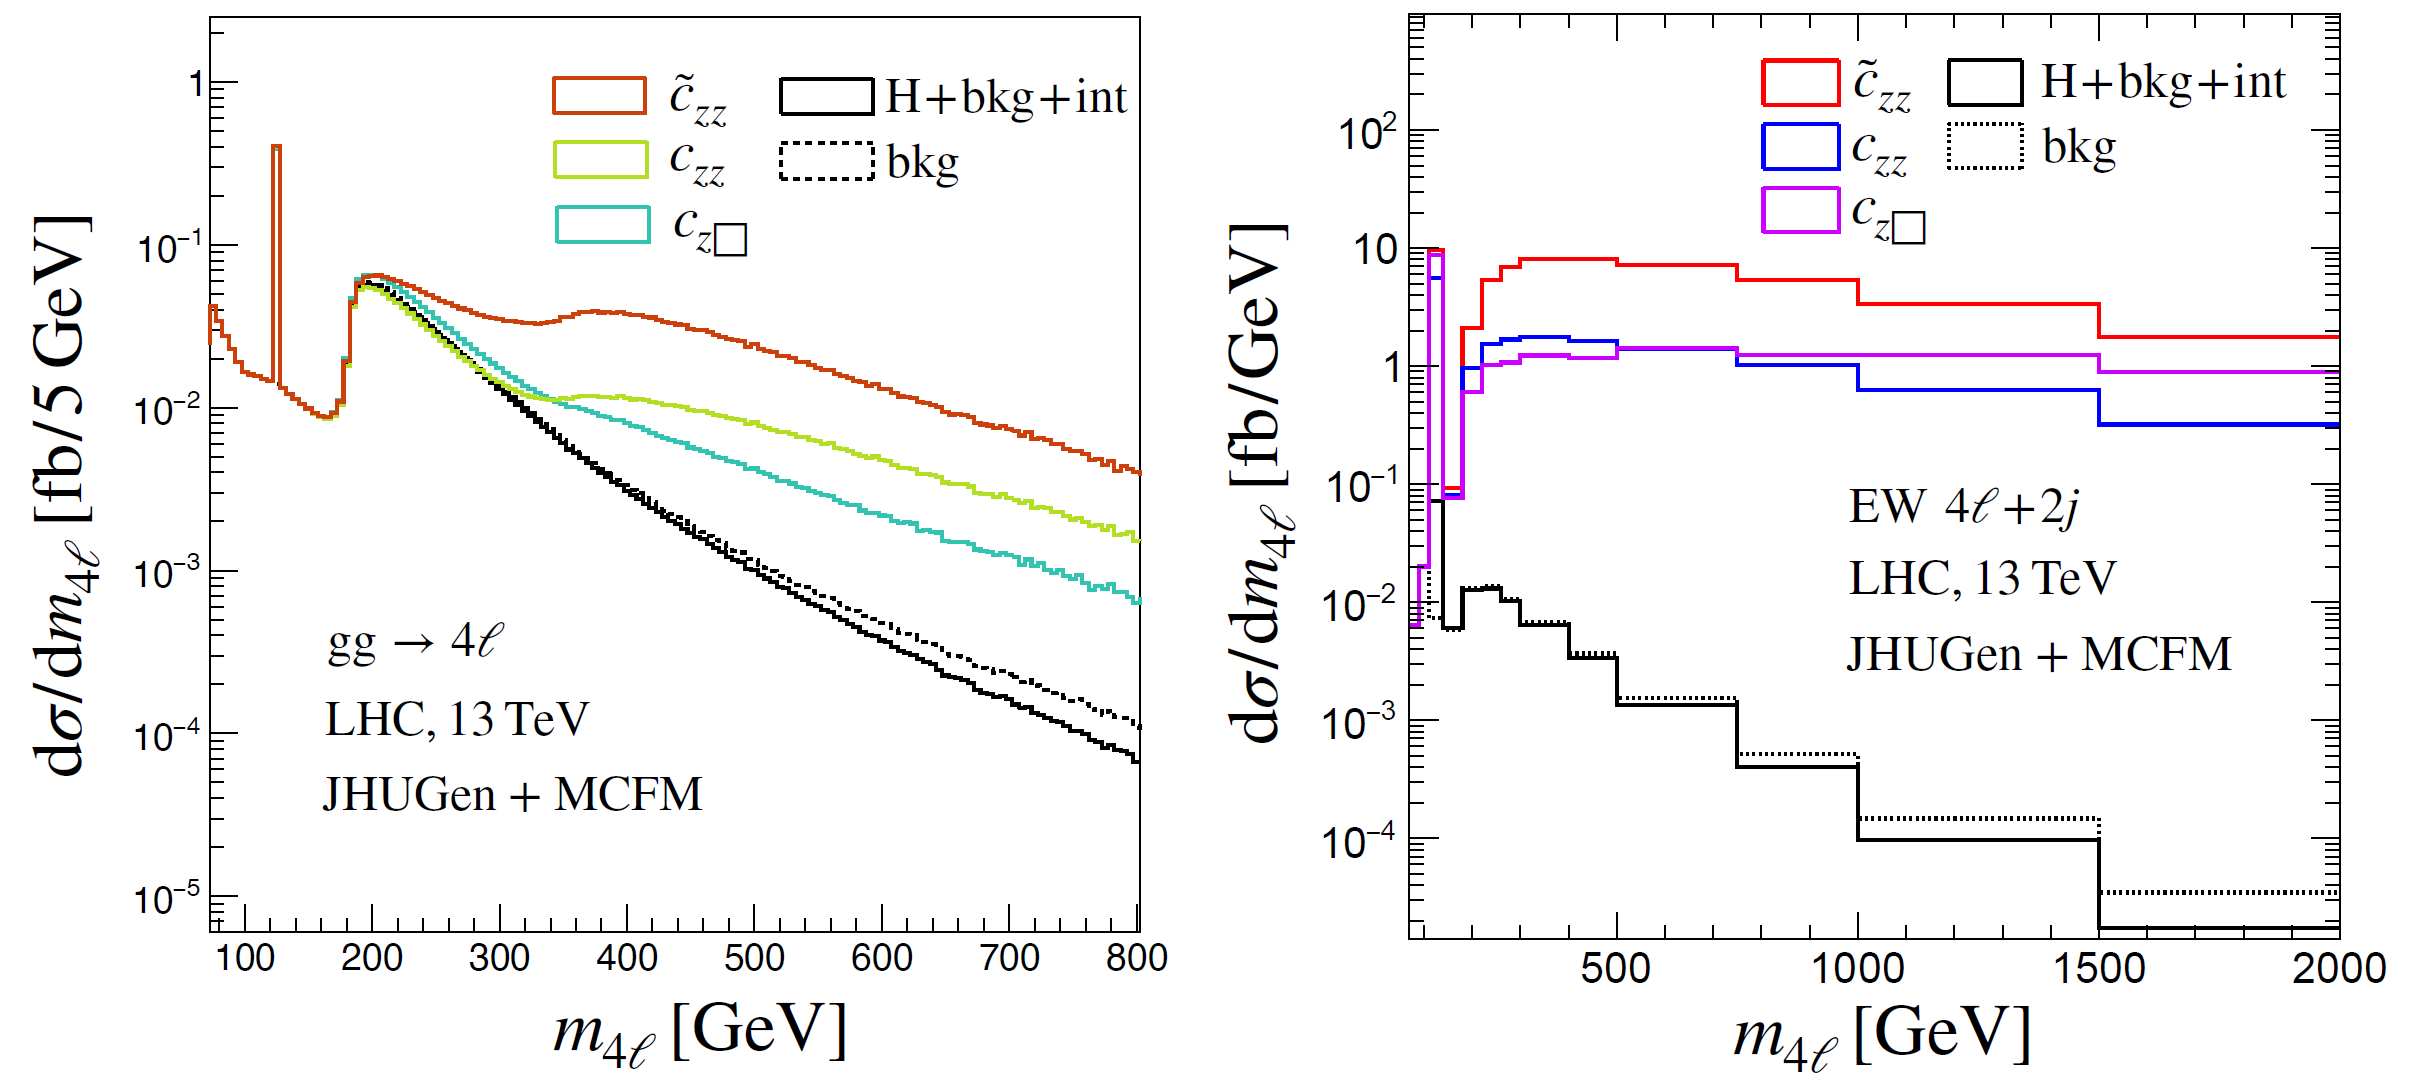
\includegraphics[width=0.85\textwidth,clip] {figures/offshellAC_BSI.png}
\caption{ The four-lepton m4$\ell$ invariant mass distributions for gluon fusion (left) and electroweak production in association with two jets (right) at the LHC with a 13 TeV pp collision energy. The total SM production (“H+bkg+int”) and background-only (“bkg”) components are shown in black. Three operators cz (magenta), czz (blue), and $\tilde{c}$zz (red) are shown in color, as analogs of the anomalous couplings described in Section~\ref{sec:amplitudeEFT}, and they are introduced in place of the SM interaction with their strength constrained to reproduce the SM cross section of the on-shell Higgs boson signal production \cite{offshellWGnote}.}
\label{fig:offshellAC_BSI}
\end{figure}

Notably, as is done in this analysis, we can also reweight these various samples to the same SM-like hypothesis, and leverage the additional statistics to make a more precise measurement of the SM-like Higgs boson. The matrix element likelihood approach (MELA), which I will discuss further in Section~\ref{sec:mela}, is used reweight all simulated off-shell events to the SM hypothesis through modified MCFM matrix elements \cite{12077235,10073492}. This eliminates the need for out-of-the-box simulation of additional SM events by utilizing statistics from our pre-existing BSM simulations instead. Furthermore, this analysis improves on past papers \cite{190100174} by including the entire Run 2 dataset (spanning years 2016, 2017, and 2018). Table~\ref{tab:samplesDAStable} provides an accounting of the datasets used.

\begin{table}[h]
	\centering
	\resizebox{\textwidth}{!}{%
		\begin{tabular}{|l|l|}
			\hline
			Process         & Dataset Name      \\ \hline
			$gg \to H \to ZZ \to 4\ell$            & /GluGluToHiggs*ToZZTo*\_M125\_GaSM*\_13TeV\_MCFM701\_pythia8/ \\ 
			$q\bar{q} \to Hqq \to ZZqq \to 4\ell qq$    & /VBFToHiggs0*ToZZTo4l\_M125\_GaSM\_13TeV\_JHUGenV730\_MCFM701\_pythia8/ \\ 
			$q\bar{q} \to W^{\pm}H \to ZZZ\to 4\ell + X$    & /VBFToHiggs0*ToZZTo4l\_M125\_GaSM\_13TeV\_JHUGenV730\_MCFM701\_pythia8/ \\ 
			$q\bar{q} \to ZH \to ZZZ \to 4\ell + X$    & /VBFToHiggs0*ToZZTo4l\_M125\_GaSM\_13TeV\_JHUGenV730\_MCFM701\_pythia8/ \\ \hline
			
			$gg \to H \to ZZ \to 4\ell$            & /GluGluHToZZTo4L\_M*\_13TeV\_powheg2\_JHUGenV7011\_pythia8/ \\ 
			$q\bar{q} \to Hqq \to ZZqq \to 4\ell qq$    & /VBF\_HToZZTo4L\_M*\_13TeV\_powheg2\_JHUGenV7011\_pythia8/ \\
			$q\bar{q} \to W^{+}H \to ZZZ\to 4\ell + X$    &  /WplusH\_HToZZTo4L\_M*\_13TeV\_powheg2-minlo-HWJ\_JHUGenV7011\_pythia8/\\ 
			$q\bar{q} \to W^{-}H \to ZZZ\to 4\ell + X$    &  /WminusH\_HToZZTo4L\_M*\_13TeV\_powheg2-minlo-HWJ\_JHUGenV7011\_pythia8/\\ 
			$q\bar{q} \to ZH \to ZZZ \to 4\ell + X$    & /ZH\_HToZZ\_4LFilter\_M*\_13TeV\_powheg2-minlo-HZJ\_JHUGenV7011\_pythia8/ \\ 
			$t\bar{t} \to H \to ZZ \to 4\ell$    & 	/ttH\_HToZZ\_4LFilter\_M*\_13TeV\_powheg2\_JHUGenV7011\_pythia8/ \\ \hline
			
			$q\bar{q} \to Hqq \to ZZqq \to 4\ell qq$    & /VBFToHiggs0PMContinToZZTo*JJ\_M125\_GaSM\_13TeV\_phantom\_pythia8/ \\ 
			$q\bar{q} \to Hqq \to ZZqq \to 4\ell qq$    & /ZZJJTo4L\_EWK\_TuneCP5\_13TeV-madgraph-pythia8/ \\ \hline
			
			$gg \to H \to ZZ \to 4\ell$            & /Higgs0PMToZZTo4L\_M125\_13TeV\_powheg2\_JHUGenV7011\_pythia8/ \\ 
			$q\bar{q} \to Hqq \to ZZqq \to 4\ell qq$    & /VBFHiggs0PMToZZTo4L\_M125\_13TeV\_JHUGenV7011\_pythia8/ \\ 
			$q\bar{q} \to W^{\pm}H \to ZZZ\to 4\ell + X$    & /WHiggs0PMToZZTo4L\_M125\_13TeV\_JHUGenV7011\_pythia8/ \\ 
			$q\bar{q} \to ZH \to ZZZ \to 4\ell + X$    & /ZHiggs0PMToZZ\_4LFilter\_M125\_13TeV\_JHUGenV7011\_pythia8/ \\ \hline
			
			$qq \to ZZ \to 4\ell$                           & /ZZTo4L\_13TeV\_powheg\_pythia8/ \\ \hline
		\end{tabular}%
	}
	\caption{Table of datasets used for Higgs production and $ZZ \to 4\ell$ decay modes.}
	\label{tab:samplesDAStable}
\end{table}

% Here, we have documented inputs used to generate samples that include on-shell events. 
There already exist on-shell samples (centered around the 125 GeV Higgs peak) for our dominant production modes generated with POWHEG v2 and JHUGen v7.0.11, which have been validated and utilized in CMS analyses~\cite{Sirunyan:2019twz, Sirunyan:2021rug, Sirunyan:2765059} so we can inherit them to use for our on-shell Higgs boson cross-section, and as a reliable point of comparison for newly generated MC events. We also have as additional samples for electroweak production, on-shell samples generated with JHUGen+JHUGenMELA and off-shell samples of the combined BSI (background+signal+interference) events via Phantom.

These samples are valuable in the validation of the recently produced off-shell samples for gluon fusion and electroweak production, which were generated using JHUGen v7.3.0 interfaced to MCFM v7.0.1 and MCFM v7.0.6. It is important to note here, as we compare on-shell events between all these samples using the cross-section and branching ratio values from Yellow Report (YR) 4, that the off-shell samples share common generator inputs which are not applied to the on-shell samples. These cuts and their associated efficiencies are documented in Table~\ref{tab:geninputtable}.

\begin{table}[h]
	\centering
	\resizebox{\textwidth}{!}{%
		\begin{tabular}{|c|c|c|c|}
			\hline
			Generator           &Sample / Analysis          & Leptons                   & Jets                                \\ \hline
			{JHUGen+MCFM}         &EW off-shell & $pT$ $l_{1,2,3,4} > 3 GeV$, $|\eta$ $l_{1,2,3,4}| < 2.7$ & $pT$ $j_{1,2} >$ 15 GeV, $m_{jj} > $30 GeV, $|\eta$ $j_{1,2}| <$ 6.5, $\Delta R$ $>$ 0.3, $|\Delta\eta$ $j_{1,2}| >$0 \\  
			
			&ggH off-shell  & $pT$ $l_{1,2,3,4} > 3 GeV$, $|\eta$ $l_{1,2,3,4}| < 2.7$ & $pT$ $j_{1,2} >$ 15 GeV, $\Delta R$ $>$ 0.4                   \\ \hline
			
			POWHEG+JHUGen                &VBF on-shell  & No specified cuts         & No specified cuts                   \\ 
			&W$^{-}$H on-shell  & No specified cuts         & No specified cuts                   \\ 
			&W$^{+}$H on-shell  & No specified cuts         & No specified cuts                   \\ 
			&ZH on-shell  & No specified cuts         & No specified cuts                   \\ 
			&ggH on-shell & No specified cuts         & No specified cuts                   \\ \hline
			
			JHUGen+JHUGen           &VBF on-shell         & No specified cuts         & $pT$ $j_{1,2} > 0$ GeV, $\Delta R > 0$ \\ 
			&WH on-shell         & No specified cuts         & No specified cuts \\ 
			&ZH on-shell         & No specified cuts         & No specified cuts \\ \hline
			
			Phantom         &EW off-shell (BSI, $4e$) & $pT$ $l_{1,2,3,4} >$ 3 GeV, $|\eta$ $l_{1,2,3,4}| < 2.7$ & $m_{jj} > $30 GeV, $|\eta$ $j_{1,2}| <$ 6.5            \\ 
			&EW off-shell (BSI, $4\mu$) & $pT$ $l_{1,2,3,4} >$ 3 GeV, $|\eta$ $l_{1,2,3,4}| < 2.7$ & $m_{jj} > $30 GeV, $|\eta$ $j_{1,2}| <$  6.5            \\ 
			&EW off-shell (BSI, $2e2\mu$) & $pT$ $l_{1,2,3,4} >$ 3 GeV, $|\eta$ $l_{1,2,3,4}| < 2.7$ & $m_{jj} > $30 GeV, $|\eta$ $j_{1,2}| <$ 6.5            \\ \hline
			
		\end{tabular}%
	}
	\caption{Generator-level cuts on jets and leptons in all utilized samples.}
	\label{tab:geninputtable}
\end{table}


% \begin{table}[h]
% 	\centering
% 	\resizebox{\textwidth}{!}{%
% 		\begin{tabular}{|c|c|c|c|}
% 			\hline
% 			Generator           &Sample / Analysis          & Leptons                   & Jets                                \\ \hline
% 			{JHUGen+MCFM}         &EW off-shell & $pT$ $l_{1,2,3,4} > 3 GeV$, $|\eta$ $l_{1,2,3,4}| < 2.7$ & $pT$ $j_{1,2} >$ 15 GeV, $m_{jj} > $30 GeV, $|\eta$ $j_{1,2}| <$ 6.5, $\Delta R$ $>$ 0.3, $|\Delta\eta$ $j_{1,2}| >$0, $sgn(\eta$ $j_{1}) = \pm sgn(\eta$ $j_{2})$ \\  
			
% 			&ggH off-shell  & $pT$ $l_{1,2,3,4} > 3 GeV$, $|\eta$ $l_{1,2,3,4}| < 2.7$ & $pT$ $j_{1,2} >$ 15 GeV, $\Delta R$ $>$ 0.4                   \\ \hline
			
% 			POWHEG+JHUGen                &VBF on-shell  & No specified cuts         & No specified cuts                   \\ 
% 			&W$^{-}$H on-shell  & No specified cuts         & No specified cuts                   \\ 
% 			&W$^{+}$H on-shell  & No specified cuts         & No specified cuts                   \\ 
% 			&ZH on-shell  & No specified cuts         & No specified cuts                   \\ 
% 			&ggH on-shell & No specified cuts         & No specified cuts                   \\ \hline
			
% 			JHUGen+JHUGen           &VBF on-shell         & No specified cuts         & $pT$ $j_{1,2} > 0$ GeV, $\Delta R > 0$ \\ 
% 			&WH on-shell         & No specified cuts         & No specified cuts \\ 
% 			&ZH on-shell         & No specified cuts         & No specified cuts \\ \hline
			
% 			Phantom         &EW off-shell (BSI, $4e$) & $pT$ $l_{1,2,3,4} >$ 3 GeV, $|\eta$ $l_{1,2,3,4}| < 2.7$ & $m_{jj} > $30 GeV, $|\eta$ $j_{1,2}| <$ 6.5            \\ 
% 			&EW off-shell (BSI, $4\mu$) & $pT$ $l_{1,2,3,4} >$ 3 GeV, $|\eta$ $l_{1,2,3,4}| < 2.7$ & $m_{jj} > $30 GeV, $|\eta$ $j_{1,2}| <$  6.5            \\ 
% 			&EW off-shell (BSI, $2e2\mu$) & $pT$ $l_{1,2,3,4} >$ 3 GeV, $|\eta$ $l_{1,2,3,4}| < 2.7$ & $m_{jj} > $30 GeV, $|\eta$ $j_{1,2}| <$ 6.5            \\ \hline
			
% 		\end{tabular}%
% 	}
% 	\caption{Table of generator-level cuts on jets and leptons in JHUGen off-shell samples.}
% 	\label{tab:geninputtable}
% \end{table}

All \offshell production simulations are conducted at LO in QCD, with higher-order corrections 
included through a $K$ factor. In the gluon fusion process, the factorization and renormalization scales are set to run dynamically by equating them to $m_{4\ell}/2$. To incorporate higher-order QCD corrections, signal cross section calculations are performed at leading order (LO), next-to-leading order (NLO), and next-to-next-to-leading order (NNLO) using the MCFM and HNNLO 2 programs~\cite{Catani:2007vq,Grazzini:2008tf,Grazzini:2013mca} under the narrow-width approximation, covering a broad range of masses spanning both the on-shell and off-shell regions.

The ratios of NNLO to LO cross sections, referred to as NNLO-to-LO $K$ factors, are used to reweight~\cite{deFlorian:2016spz} the $m_{4\ell}$ distributions obtained from LO QCD simulations produced with MCFM and JHUGen. A constant $K$ factor of 1.10 is applied across the entire $m_{4\ell}$ spectrum to normalize the Higgs boson production cross section via gluon fusion to the next-to-next-to-next-to-leading order (N$^3$LO) prediction at $m_{4\ell} \approx 125$\,GeV~\cite{deFlorian:2016spz}. The $m_{4\ell}$ distributions from the POWHEG+JHUGen simulation of the $gg \to H$ process are reweighted using NNLO-to-NLO $K$ factors.

While the NNLO-to-LO $K$ factor is directly applicable to the signal, it serves only as an approximation for the $gg \to 4\ell$ background and its interference with the signal. An approximate NLO calculation~\cite{Caola:2015psa,Melnikov:2015laa,Campbell:2016ivq,Caola:2016trd} is available for both the background and the interference. The resulting NLO-to-LO $K$ factors for these components agree with the signal $K$ factor within approximately 10\% in the $m_{4\ell} > 220$\,GeV range relevant to this analysis. Consequently, the same NNLO-to-LO $K$ factor and N$^3$LO normalization, computed for the signal, are applied to the background and interference, along with their associated uncertainties. An additional 10\% uncertainty is assigned to the background component, and a 5\% uncertainty—corresponding to the square root of the variation—is applied to the interference.

The $q\bar{q} \to 4\ell$ background is simulated at NLO in QCD and LO in electroweak (EW) theory using POWHEG. The fully differential cross section for this process has been computed at NNLO in QCD~\cite{Grazzini:2015hta}, and a differential NNLO-to-NLO $K$ factor as a function of $m_{4\ell}$ is applied to the POWHEG sample. This $K$ factor is approximately 1.1 at $m_{4\ell} = 125$\,GeV and varies between 1.0 and 1.2 in the region $m_{4\ell} < 500$\,GeV. The uncertainty from missing EW corrections in the low-mass region ($m_{4\ell} < 2m_{Z}$) is small compared to QCD-related uncertainties.

To account for EW corrections, an NLO-to-LO $K$ factor~\cite{Bierweiler:2013dja} is applied to events containing two on-shell Z bosons. This $K$ factor decreases with increasing $m_{4\ell}$, from approximately 1.0 near 125\,GeV to around 0.9 in the high-mass region ($m_{4\ell} > 500$\,GeV). The associated uncertainty is the dominant systematic for the off-shell width measurement and is included as a function of $m_{4\ell}$.

% In the on-shell region, the EW background from $VVV$, $t\bar{t}VV$, and $t\bar{t}V$ processes is generated using MadGraph5\_aMC@NLO~\cite{Alwall:2014hca}.

\section{Matrix Element Likelihood Approach} \label{sec:mela}

With up to 13 observables ($\boldsymbol{\Omega}$) describing the \Hboson kinematic distributions in the $2\to 6$ process, as visualized in Figure~\ref{fig:MELA}, it can be a challenging task to perform an optimal analysis. %in a multidimensional space of observables. 
MELA lets us calculate the matrix elements (ME) for each Higgs boson interaction as a function of its couplings and interacting particles. We can utilize these ME in ratios to change our hypotheses and reweight our Monte-Carlo samples, or treat them as probabilities and construct discriminants from the ME to use as observables (as discussed further in Section~\ref{sec:categories}). 

\begin{figure}[!htb]
\centering
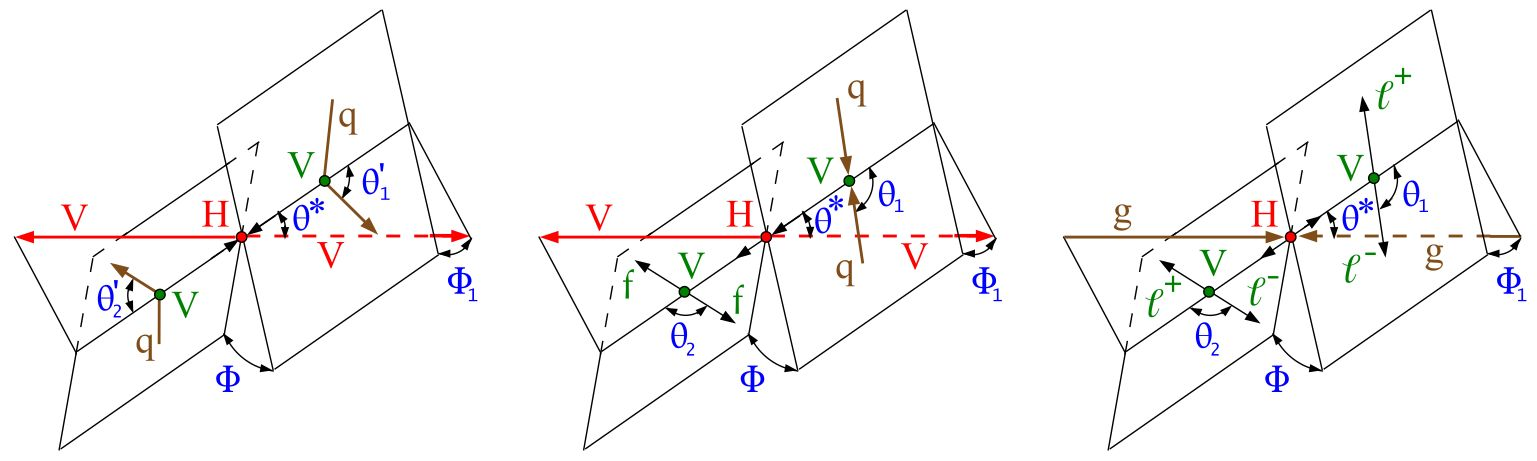
\includegraphics[width=0.8\textwidth,clip] {figures/MELA.jpg}
\caption{Diagrams of relevant kinematic observables in VBF (left), VH (center), and ggH (right) production modes of the Higgs boson.}
\label{fig:MELA}
\end{figure}

The MELA approach is designed to reduce the number of observables to the minimum while retaining all essential information. This is a very powerful tool which ensures that our analysis observables are still based in first principles, while affording us the flexibility to reweight distributions to new hypotheses or combine differently simulated statistics for greater precision in a single measurement. 

% In order to perform a dedicated study of the particular kinematic topology of HVV, visualized in \ref{fig:MELA}, events are split into several mutually 
% exclusive categories based on the presence of other particles produced in association with the \Hboson candidate~\cite{Sirunyan:2021rug}.
% We use the values of kinematic discriminants, and other selection requirements to perform the categorization. 

% \begin{figure}[!htb]
% \centering
% 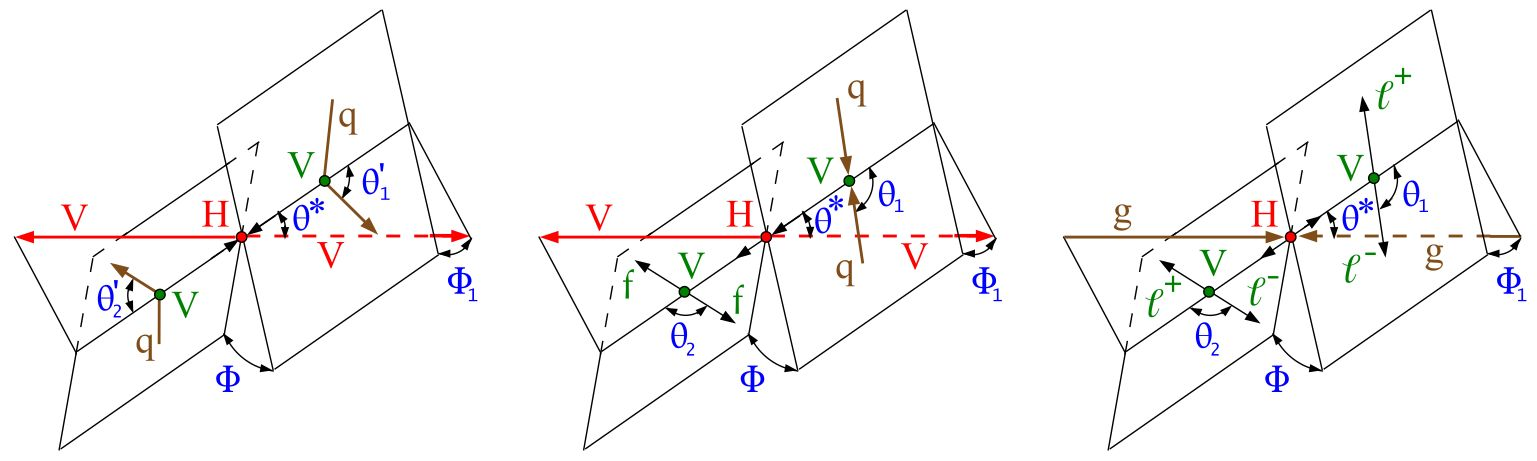
\includegraphics[width=0.8\textwidth,clip] {figures/MELA.jpg}
% \caption{Diagrams of relevant kinematic observables in VBF (left), VH (center), and ggH (right) productions of the Higgs boson.}
% \label{fig:MELA}
% \end{figure}

% The definition of these discriminants can be found in Refs.~\cite{Sirunyan:2017exp,Sirunyan:2017tqd,Sirunyan:2019twz,Sirunyan:2021rug}. 
% They are calculated using the MELA approach while employing the matrix elements at leading order (LO) in quantum chromodynamics (QCD). 

% \begin{equation}
% \mathcal{D}_\mathrm{alt}\left(\boldsymbol{\Omega}\right) = \frac{\mathcal{P}_\text{sig}\left(\boldsymbol{\Omega}\right) }
% {\mathcal{P}_\text{sig}\left(\boldsymbol{\Omega}\right) +\mathcal{P}_\mathrm{alt}\left(\boldsymbol{\Omega}\right) }
% \label{eq:melaD}
% \end{equation}

% \begin{equation}
% \mathcal{D}_\mathrm{int}\left(\boldsymbol{\Omega}\right) =
% \frac{\mathcal{P}_\mathrm{int}\left(\boldsymbol{\Omega}\right) }
% {2 \ \sqrt{{\mathcal{P}_\text{sig}\left(\boldsymbol{\Omega}\right) \ \mathcal{P}_\mathrm{alt}\left(\boldsymbol{\Omega}\right) }}}
% \label{eq:melaDint}
% \end{equation}

% These discriminants use full kinematic information from the \Hboson and from associated jet production and 
% are labeled to indicate a specific topology (2jet) and production mechanism (VBF, WH, ZH), 
% which is discriminated against the dominant gluon fusion process:
% %$\mathcal{D}_\mathrm{1jet}^{VBF}$, 
% $\mathcal{D}_\mathrm{2jet}^{VBF}$, 
% $\mathcal{D}_\mathrm{2jet}^{ZH}$,
% and $\mathcal{D}_\mathrm{2jet}^{WH}$. 
% %The $\mathcal{D}_\mathrm{2jet}$ discriminants are calculated using both SM and anomalous coupling hypotheses, 
% %leading to a set $\mathcal{D}_\mathrm{2jet}^{i}$, all of which 
% %are tested in order to maintain high efficiency of VBF and VH categorization in the presence of anomalous couplings. 
% % Calculation of these discriminants is discussed in more detail later with the presented analysis. 

% % The MELA approach also allows for reweighting between our simulated probability distributions. This has the effect of reducing the number of dedicated 
% % Monte-Carlo simulations required for this analysis, as well as bolstering the available statistics that can be utilized in our templates for Bayesian analysis. 

% \begin{figure}
% \centering
% 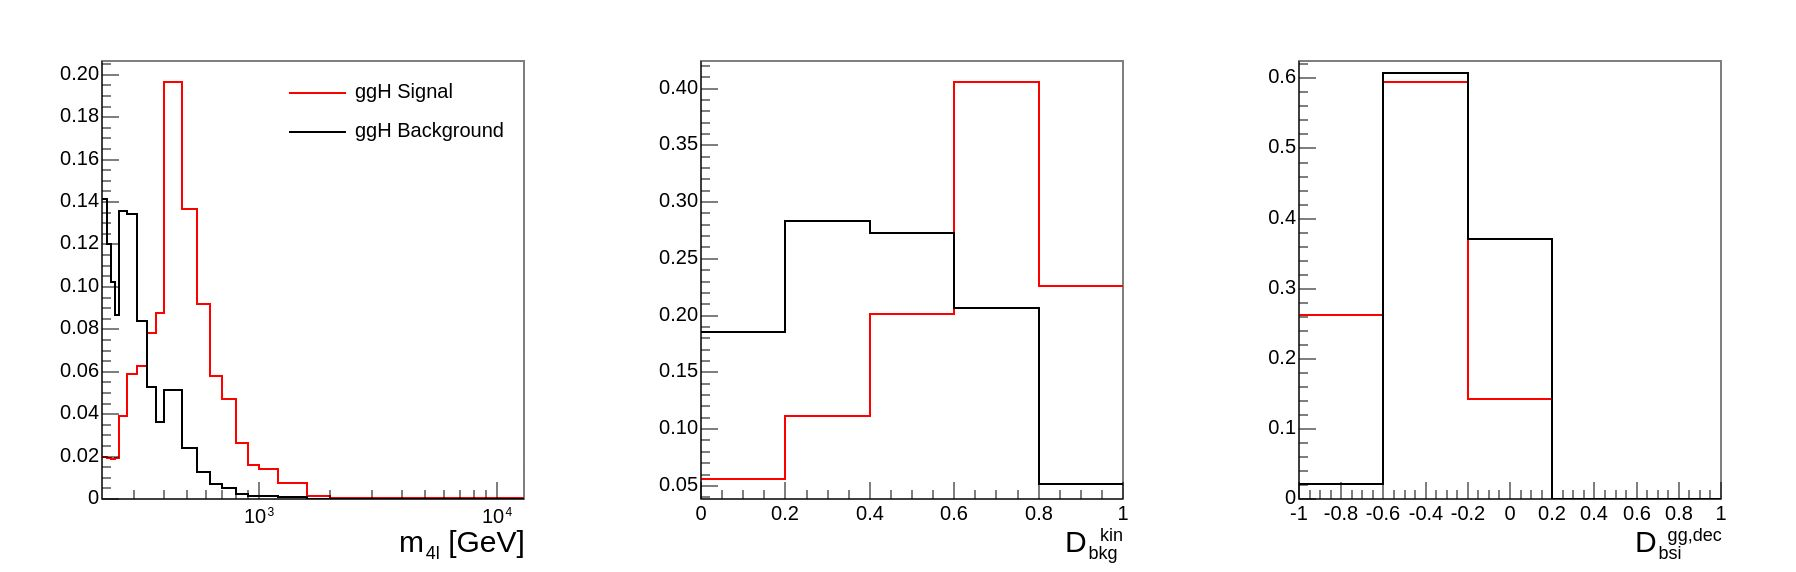
\includegraphics[width=0.8\textwidth,clip] {figures/DiscDists.jpg}
% \caption{}
% \label{fig:DiscDists}
% \end{figure}

\section{Building a $H^{(*)} \to ZZ^{(*)} \to 4\ell$ analysis}

\subsection{Reconstructing and Selecting events} \label{sec:recoandsel}

% Event reconstruction is based on the particle-flow (PF) algorithm~\cite{Sirunyan:2017ulk}. This algorithm aims to reconstruct and identify each individual particle in an event, with an optimized combination of information from the various elements of the CMS detector. The energy of photons is obtained from the ECAL measurement. The energy of electrons is determined from a combination of the electron momentum at the primary vertex as determined by the tracker, the energy of the corresponding ECAL cluster, and the energy sum of all bremsstrahlung photons spatially compatible with originating from the electron track. The energy of muons is obtained from the curvature of the corresponding track. The energy of charged hadrons is determined from a combination of their momentum measured in the tracker and the matching ECAL and HCAL energy deposits, corrected for the response function of the calorimeters to hadronic showers. Finally, the energy of neutral hadrons is obtained from the corresponding corrected ECAL and HCAL energies.

% Muons with $p_T > 5$ GeV are reconstructed within the geometrical acceptance, corresponding to the region $|\eta|< 2.4$, by combining information from the silicon tracker and the muon systems \cite{MuReco}. The muons are selected among the reconstructed muon track candidates by applying quality requirements on the track in both the muon and silicon tracker systems, and demanding small energy deposits in the calorimeters.

Event reconstruction is based on the particle-flow (PF) algorithm~\cite{Sirunyan:2017ulk}, which endeavors to reconstruct and identify each individual particle in an event by combining information from the various subdetectors of the CMS experiment. PF candidates are classified as photons, electrons, muons, or charged or neutral hadrons, and they are then used to build higher-level objects, such as jets. 

Photon energies are determined directly from ECAL measurements, and are not expected to present a signal in the HCAL or tracker. Electrons are identified from a multivariate discriminant involving their momentum at the PV as measured by the tracker, a geometrically corresponding ECAL cluster of energy deposition, and the integrated energy of all bremsstrahlung (radiated) photons determined to be spatially consistent with emission from the electron's trajectory~\cite{Sirunyan:2021rug}. Muons, like electrons, also start in the tracker, but have trajectories and momenta that can be extrapolated to the muon system while depositing little to no energy in the ECAL and HCAL. Their energies are inferred from the curvature of their tracks in the magnetic field. After the isolated muons, electrons, and photons are classified, the remaining particles are used to identify hadrons. For charged hadrons, energies are determined by combining their momenta measured in the tracker with the corresponding ECAL and HCAL energy deposits. The energies of neutral hadrons are obtained from their corrected ECAL and HCAL energy deposits.

Electrons are reconstructed within the geometrical acceptance defined by $|\eta| < 2.5$ and transverse momentum $p_{\mathrm{T}} > 7$\,GeV~\cite{eleReco}. While muons with transverse momentum $p_T > 5$ GeV are reconstructed within the geometrical acceptance of $|\eta|< 2.4$. Candidates are reconstructed using information from both the silicon tracker and the muon detection systems~\cite{MuReco}. Then, the selection of muons from among the reconstructed muon track candidates is subject to stringent quality criteria applied to tracks in both the muon chambers and the silicon tracker, complemented by requirements of minimal energy deposition in the calorimeter systems, ensuring high purity in the muon identification.

Additionally, to distinguish prompt lepton products of high-$p_T$ $Z$ boson decays from those originating in hadronic jets---such as leptons produced in electroweak decays of hadrons---an isolation requirement is applied. For muons, an isolation variable is computed to quantify the level of surrounding activity and suppress backgrounds from non-prompt sources~\cite{Sirunyan:2021rug}. The isolation variable is defined relative to the muon's transverse momentum $p_T$ as
\begin{equation} \label{eqn:pfiso}
  {\mathcal I}^{\mu} \equiv \Big( \sum p_T^\text{charged} + \max\big[ 0, \sum p_T^\text{neutral} +
    \sum p_T^{\gamma} - p_T^{\mathrm{PU}} \big] \Big) / p_T,
\end{equation}
where $p_T^{\text{charged}}$, $p_T^\text{neutral}$, and $p_T^\gamma$ are summed over the charged and neutral hadrons and photons within a cone radius of $\Delta R \equiv \sqrt{\smash[b]{(\eta^i-\eta^j)^{2} + (\phi^i-\phi^j)^{2}}} = 0.3$ around the lepton's direction at the interaction vertex. Here, $\phi$ denotes the azimuthal angle and indices $\textit{i}$ and $\textit{j}$ refer to the hadron or photon and muon, respectively. This isolation variable exhibits particular sensitivity to energy deposits from pileup interactions. Therefore, a contribution $p_T^{\mathrm{PU}}$ from pileup is subtracted, as seen in Equation~(\ref{eqn:pfiso})~\cite{PUmitigationCMS}. Finally, each muon in a selected event must satisfy ${\mathcal{I}^{\mu}} < 0.35$.
% This term is defined as $p_T^{\mathrm{PU}} = 0.5\sum_{i}p_T^{i,\mathrm{PU}}$, involving the sum of $p_T$ over all charged hadrons $i$ not originating from the PV, where the factor of 0.5 accounts for the differing fractions of charged and neutral hadrons~\cite{PUmitigationCMS}. 

Instead of applying a separate isolation requirement---as in the case for muons---the electron multivariate discriminant incorporates the isolation sums ($\sum p_{\mathrm{T}}^{\text{charged}}$, $\sum p_{\mathrm{T}}^{\text{neutral}}$, and $\sum p_{\mathrm{T}}^{\gamma}$) directly~\cite{Sirunyan:2021rug}. The inclusion of these isolation components offers better performance for electrons compared to a simple threshold on the relative isolation variable. XGBOOST is used on simulated events to train and optimize the multivariate discriminant employed for electron identification and isolation. Events are separated into six regions, defined by two transverse momentum ranges ($7 < p_{\mathrm{T}} < 10$\,GeV and $p_{\mathrm{T}} > 10$\,GeV) and three pseudorapidity intervals: the central barrel ($|\eta_{e}| < 0.8$), outer barrel ($0.8 < |\eta_{e}| < 1.479$), and endcaps ($1.479 < |\eta_{e}| < 2.5$). Separate discriminant training is performed for each of the three data-taking periods in Run 2, and the selection requirements are optimized such that the signal efficiency is uniform across all three periods.

The effect of the final-state radiation (FSR) from leptons are also recovered~\cite{Sirunyan:2017ulk}. (Bremsstrahlung photons already associated to electrons in the reconstruction step are not considered.) Isolated photons satisfying $p_T^\gamma>2$ GeV, $|\eta^\gamma| <2.4$, and $\mathcal{I}^{\gamma} < 1.8$ are associated with the nearest selected lepton (muon or electron) in the event. Photons must also satisfy the criteria $\Delta R(\gamma,\ell)/(p_T^{\gamma})^2<0.012~\text{GeV}^{-2}$ and $\Delta R(\gamma,\ell) < 0.5$. When multiple photon candidates fulfill these conditions, the one minimizing $\Delta R(\gamma,\ell)/(p_T^{\gamma})^2$ with respect to the given lepton is retained. FSR photons are excluded from the computation of the relative isolation parameter.

% Electrons with $p_T>7$ GeV are reconstructed within the geometrical acceptance, defined by the pseudorapidity region $|\eta|<2.5$~\cite{eleReco}. Their identification utilizes a multivariate discriminant incorporating observables sensitive to bremsstrahlung emission along the electron trajectory, the geometric and momentum-energy matching between the electron trajectory and associated ECAL cluster, the electromagnetic shower morphology in the ECAL, and variables discriminating against electrons originating from photon conversions. Electron isolation parameters, defined analogously to those for muons, are integrated into this multivariate discriminant to differentiate between prompt leptons from Z boson decays and those arising from electroweak decays of hadrons within jets. The XGBoost package~\cite{xgboost} is employed for training and optimization of this multivariate discriminant using simulated events that remain independent from all other analysis stages. Separate training procedures are implemented for each of the three data-taking periods \cite{ElectronBDT}. Electrons from photon conversions and muons from in-flight hadronic decays are rejected if the ratio of their three-dimensional impact parameter, computed with respect to the primary vertex position, to its uncertainty exceeds four.



A ``tag-and-probe'' technique~\cite{CMS:2011aa}, based on samples of $Z$ boson events in both data and simulation, is employed to measure the reconstruction and selection efficiencies for prompt electrons and muons across bins of transverse momentum ($p_{\mathrm{T}}$) and pseudorapidity ($\eta$). The differences between the efficiencies measured in data and those obtained from simulation are used to derive correction factors, which are applied to rescale the event yields in the simulated samples~\cite{Sirunyan:2021rug}. These simulated events are also utilized to calibrate the momentum scale and resolution of prompt leptons, again in bins of $p_{\mathrm{T}}$ and $\eta$~\cite{ScaleSmear2, Roch2}.


% The reconstruction and selection efficiencies for prompt leptons in both data and simulation are evaluated using a tag-and-probe technique~\cite{CMS:2011aa} applied to $Z$ boson event samples. The ratio of efficiencies measured in data to those in simulation is applied as a correction factor to the yields of selected events in the simulated samples.


For this analysis, selection of Higgs boson candidates requires four prompt and isolated leptons following the aforementioned criteria. One lepton must satisfy $p_T>20$ GeV and at least one additional lepton must have $p_T>10$ GeV. Then, Z boson candidates are constructed from $e^+e^-$ or $\mu^+\mu^-$ pairs with invariant masses in the range 12--120 GeV. These dilepton pairs are combined to form a Higgs boson candidate. 
We choose $Z_1$ to label the pair with invariant mass closest to the nominal Z boson mass, 
and call the remaining pair $Z_2$. 

Four possible combinations are considered and treated independently: 
$4\mu$, $4e$, $2e2\mu$, and $2\mu2e$, where the mixed-flavor final states are distinguished based on the flavor composition of $Z_{1}$. These four combinations exhibit different four-lepton mass resolutions (predominantly determined by the flavor composition of $Z_{1}$) and contain different amounts of reducible background (largely dependent on the flavor composition of $Z_{2}$). Since none of these flavor-dependent characteristics impact the off-shell \Hboson analysis, all flavor channels are combined to make our measurement~\cite{PhysRevD.111.092014}. 

Signal candidates must satisfy $m_{4\ell} > 70$ GeV. When multiple \Hboson candidates can be formed in an event, the one with the highest value of the kinematic discriminant $\mathcal{D}_\text{bkg}^\text{kin}$ (defined in Section~\ref{sec:categories}) is chosen, However, if these \Hboson candidates are comprised of the same four leptons, the candidate whose $Z_1$ invariant mass lies closest to the nominal Z boson mass is selected.

In this off-shell analysis, events undergo further categorization based on jets associated with the \Hboson candidate~\cite{PhysRevD.111.092014}. Jets are clustered using the anti-$k_t$ jet finding algorithm~\cite{Cacciari:2008gp,Cacciari:2011ma} with a distance parameter of 0.4. The jet momentum is determined as the vector sum of all constituent particle momenta. 
Jets must satisfy $p_T>30$ GeV and $|\eta|<4.7$ and must be spatially separated
from all selected lepton candidates and any selected FSR photons by requiring 
$\Delta R(\ell/\gamma,\text{jet})>0.4$.
Jets originating from b quark hadronization are identified using the DeepCSV algorithm~\cite{Sirunyan:2017ezt}, which integrates information 
on impact parameter significance, secondary vertex characteristics, and jet kinematic variables. These b-tagged jets are then used as part of our criteria for categorizing events, as detailed in Section~\ref{sec:categories}.

% Here, $\Delta R(i,j) Equation \refuiv \sqrt{\smash[b]{(\eta^i-\eta^j)^{2} + (Hi^i-Hi^j)^{2}}}$, where $Hi$ is the azimuthal angle, and in this case $\textit{i}$ refers to the hadron or photon, and $\textit{j}$ to the muon.
% Since the isolation variable is particularly sensitive to energy deposits from pileup interactions, a contribution $p_T^{\mathrm{PU}}$ from pileup is subtracted from the isolation parameter, as shown in Equation~(\ref{eqn:pfiso}). 
% It is defined as 0.5 times the $p_T$ sum of all charged hadrons $i$ not originating from the primary vertex $p_T^{\mathrm{PU}} = 0.5\sum_{i}p_T^{i,\mathrm{PU}}$, where the 0.5 factor accounts for the different fraction of charged and neutral hadrons~\cite{PUmitigationCMS}. A requirement of ${\mathcal{I}^{gm}} < 0.35$ is placed on each muon in the event.

% Photons from final-state radiation are reconstructed using the PF algorithm~\cite{Sirunyan:2017ulk}. Isolated photons with $p_T >2$ GeV, $|\eta| <2.4$, and $\mathcal{I}^{\gamma} < 1.8$, are associated with the closest lepton (either muon or electron) in the event. Photons that do not satisfy the requirements $\Delta R(gg,\ell)/(p_T^{\gamma})^2<0.012 GeV^{-2}$ and $\Delta R(gg,\ell) < 0.5$ are discarded.
% If more than one photon candidate fulfils the above conditions, the one with the lowest value of $\Delta R(gg,\ell)/(p_T^{\gamma})^2$ with respect to the given lepton is retained.
% Photons passing the above criteria are excluded from the computation of the relative isolation parameter. 

% Electrons with $p_T>7$ GeV are reconstructed within the geometrical acceptance, corresponding to the pseudorapidity region $|\eta|<2.5$~\cite{eleReco}. They are identified using a multivariate discriminant, which includes observables sensitive to the emission of bremsstrahlung along the electron trajectory, the geometrical and momentum-energy matching between the electron trajectory and the associated cluster in the ECAL, the shape of the electromagnetic shower in the ECAL, and variables that discriminate against electrons originating from photon conversions. The isolation parameter sums for electrons, defined similarly as for muons, are included in the multivariate discriminant. This information is used to discriminate between prompt leptons from Z boson decays and those arising from EW decays of hadrons within jets. The package XGBoost~\cite{xgboost} is used to train and optimize this multivariate discriminant. The training is performed with simulated events that are not used at any other stage of the analysis. Separate trainings are performed for the three different data-taking periods \cite{ElectronBDT}. Electrons from photon conversions and muons from in-flight decays of hadrons are rejected if the ratio of their impact parameter in three dimensions, computed with respect to the primary vertex position, to their uncertainty is greater than four.

% The reconstruction and selection efficiencies for prompt leptons in both data and simulation have been estimated using a tag-and-probe technique~\cite{CMS:2011aa} based on samples of $Z$ boson events. The ratio of the efficiencies measured in data and simulation is used to rescale the yields of selected events in the simulated samples.
% In addition, $Z$ boson events have been used to calibrate the momentum scale and resolution of electrons and muons in bins of different kinematic variables~\cite{ScaleSmear2, Roch2}.

% In the selection of Higgs boson candidates,
% four prompt and isolated leptons are required following the prescription above. 
% One of the leptons must have $p_T>20$ GeV and at least one of the remaining leptons must satisfy $p_T>10$ GeV.
% The Z boson candidates are constructed from $epem$ or $gmpgmm$ pairs whose  invariant mass is in the range 12--120 GeV. 
% The dilepton pairs are then combined to form the Higgs boson candidate. 
% In the following, $Z_1$ denotes the pair with the mass closest to the nominal $Z$ boson mass, 
% while $Z_2$ refers to the remaining one. Four possible combinations are considered and treated separately: 
% 4gm, 4$e$, $2e2gm$, and $2gm2e$, where the mixed-flavor final states are separated based on the decay of $Z_{1}$. 
% The four possible combinations have different four-lepton mass resolutions (largely driven by whether the $Z_{1}$ is formed from 2$gm$ or 2$e$) 
% and different amounts of reducible background (largely driven by whether the $Z_{2}$ decays to 2$\mu$ or 2$e$).
% None of the above differences between the flavor channels affect the off-shell \Hboson analysis 
% and therefore all flavor channels are combined in that measurement. 
% Signal candidates must satisfy $m_{4\ell} > 70$ GeV. 
% If more than one \Hboson candidate can be formed in the event, the one with the highest value of the 
% kinematic discriminant $\mathcal{D}_\text{bkg}^\text{kin}$, defined in Section~\ref{sec:Discriminants},
% is retained, unless these candidates consist of the same four leptons. 
% In this case, the candidate with the $Z_1$ invariant mass closest to the nominal Z boson mass is retained.

% In the off-shell analysis, events are further categorized based on the jets associated with the \Hboson candidate. 
% The jets are clustered using the anti-\kt jet finding algorithm~\cite{Cacciari:2008gp,Cacciari:2011ma} with a distance 
% parameter of 0.4. The jet momentum is determined as the vector sum of all particle momenta in the jet. 
% Jets must satisfy $p_T>30$ GeV and $|\eta|<4.7$ and must be separated
% from all selected lepton candidates and any selected final-state radiation photons by demanding 
% $\Delta R(\ell/\cPgg,{\text{jet}})>0.4$.
% Jets originating from the hadronization of b quarks are identified using the DeepCSV algorithm~\cite{Sirunyan:2017ezt}, which combines information 
% on impact parameter significance, the secondary vertex, and jet kinematic variables. The use of this identification is described in Section~\ref{sec:Discriminants}.

























\subsection{Defining categories and observables} \label{sec:categories}

% With up to 13 observables, $\boldsymbol{\Omega}$, describing the \Hboson kinematic distributions in the $2\to 6$ process,
% it is a challenging task to perform an optimal analysis in a multidimensional space of observables. 
% The MELA approach is designed to reduce the number of observables to the minimum while retaining all essential information. 
% Two types of discriminants were defined for either the production or decay process, and we also combine them into a joint 
% discriminant for the full $2\to 6$ process where relevant.

% \begin{figure}[!htb]
% \centering
% 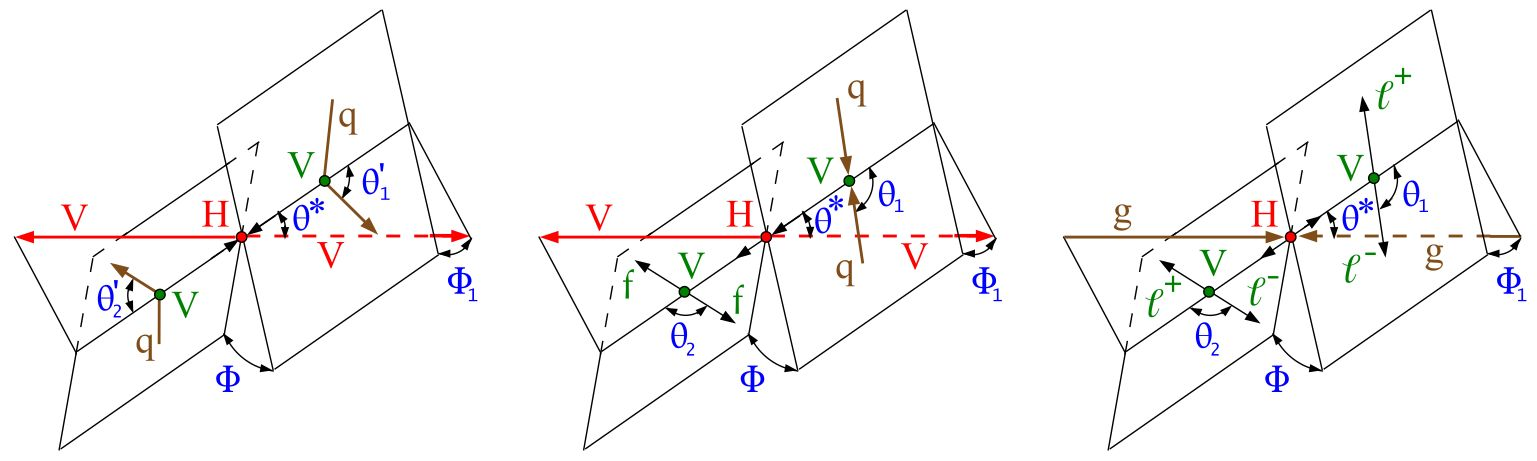
\includegraphics[width=0.8\textwidth,clip] {figures/MELA.jpg}
% \caption{Diagrams of relevant kinematic observables in VBF (left), VH (center), and ggH (right) productions of the Higgs boson.}
% \label{fig:MELA}
% \end{figure}

In order to perform a dedicated study of the particular kinematic topology of HVV, visualized in Figure~\ref{fig:MELA}, events are split into several mutually exclusive categories based on the presence of other particles produced in association with the \Hboson candidate~\cite{Sirunyan:2021rug}. Two types of discriminants are defined for either the production or decay process, which can be combined to describe the full $2\to 6$ process~\cite{Sirunyan:2017exp,Sirunyan:2017tqd,Sirunyan:2019twz,Sirunyan:2021rug}. We use the values of these kinematic discriminants and other selection requirements to perform the categorization. They are calculated using the MELA approach while employing the matrix elements at leading order (LO) in quantum chromodynamics (QCD):
\begin{equation}
	\mathcal{D}_\mathrm{alt}\left(\boldsymbol{\Omega}\right) = \frac{\mathcal{P}_\text{sig}\left(\boldsymbol{\Omega}\right) }
	{\mathcal{P}_\text{sig}\left(\boldsymbol{\Omega}\right) +\mathcal{P}_\mathrm{alt}\left(\boldsymbol{\Omega}\right) }
	\label{eq:melaD}
\end{equation}
\begin{equation}
	\mathcal{D}_\mathrm{int}\left(\boldsymbol{\Omega}\right) =
	\frac{\mathcal{P}_\mathrm{int}\left(\boldsymbol{\Omega}\right) }
	{2 \ \sqrt{{\mathcal{P}_\text{sig}\left(\boldsymbol{\Omega}\right) \ \mathcal{P}_\mathrm{alt}\left(\boldsymbol{\Omega}\right) }}},
	\label{eq:melaDint}
\end{equation}

where the probability of a certain process $\mathcal{P}$ is calculated using the full kinematics characterized
by $\boldsymbol{\Omega}$ for the hypotheses denoted as ``sig'' for a signal model and ``alt'' for an alternative model,
which could be an alternative \Hboson production mechanism (used to categorize events),
background (used to isolate signal), or an alternative \Hboson coupling model (used to measure coupling parameters).
The ``int'' label represents the interference between the two model contributions.
The probabilities $\mathcal{P}$ are calculated from the matrix elements provided by the MELA package and
are normalized to give the same integrated cross sections in the relevant phase space of each process.

% These discriminants use full kinematic information from the \Hboson with its associated jets and 
% are labeled to indicate a specific topology (2jet) and production mechanism (VBF, WH, ZH), 
% which is discriminated against the dominant gluon fusion process:
% %$\mathcal{D}_\mathrm{1jet}^{VBF}$, 
% $\mathcal{D}_\mathrm{2jet}^{VBF}$, 
% $\mathcal{D}_\mathrm{2jet}^{ZH}$,
% and $\mathcal{D}_\mathrm{2jet}^{WH}$. 

%The $\mathcal{D}_\mathrm{2jet}$ discriminants are calculated using both SM and anomalous coupling hypotheses, 
%leading to a set $\mathcal{D}_\mathrm{2jet}^{i}$, all of which 
%are tested in order to maintain high efficiency of VBF and VH categorization in the presence of anomalous couplings. 
% Calculation of these discriminants is discussed in more detail later with the presented analysis. 

% The MELA approach also allows for reweighting between our simulated probability distributions. This has the effect of reducing the number of dedicated 
% Monte-Carlo simulations required for this analysis, as well as bolstering the available statistics that can be utilized in our templates for Bayesian analysis. 
 
A set of discriminants $\mathcal{D}_\text{2jet}$ is constructed, following Equation \ref{eq:melaD},
where $\mathcal{P}_\text{sig}$ corresponds to the signal probability for the VBF ($WH$ or $ZH$)
production hypothesis in the VBF-tagged (VH-tagged) category, and $\mathcal{P}_\mathrm{alt}$
corresponds to that of \Hboson production in association with two jets via gluon fusion.
These discriminants use full kinematic information from the \Hboson with its associated jets and 
are labeled to indicate a specific topology (2jet) and production mechanism (VBF, WH, ZH), 
which is discriminated against the dominant gluon fusion process:
$\mathcal{D}_\mathrm{2jet}^{VBF}$, 
$\mathcal{D}_\mathrm{2jet}^{ZH}$,
and $\mathcal{D}_\mathrm{2jet}^{WH}$.
When more than two jets pass the selection criteria, the two jets with the highest $p_T$ are chosen 
for the matrix element calculations. Thus, the $\mathcal{D}_\text{2jet}$ discriminants separate the 
target production mode of each category from gluon fusion production,
in all cases using only the kinematics of the \Hboson and two associated jets~\cite{PhysRevD.111.092014}.

% Sequential selection criteria are used to define the categories:
% \begin{itemize}
%     \item[--]  The VBF-2jet category requires exactly four leptons. In addition, there must be 
%     either two or three jets of which at most one is identified as coming from the hadronization of a b quark, which we term a b-tagged jet~\cite{Sirunyan:2021rug}, 
%     or at least four jets and no b-tagged jets. 
%     Finally, $\mathcal{D}_\text{2jet}^{VBF} >0.5$ is required~\cite{Sirunyan:2021rug}. 
    
%     \item[--]  The VH-hadronic category requires exactly four leptons. In addition, there must be
%     either two or three jets, or at least four jets and no b-tagged jets. 
%     Finally, we demand $\max(\mathcal{D}_\text{2jet}^{WH},~\mathcal{D}_\text{2jet}^{ZH} )>0.5$~\cite{Sirunyan:2021rug}.
    
%     \item[--]  The Untagged category consists of the remaining events.
% \end{itemize}

Sequential selection criteria are used to define the event categories:
\begin{itemize}
    \item[--] The VBF-2jet category requires exactly four leptons. In addition, events must contain either two or three jets with at most one identified as originating from a b quark (b-tagged jet)~\cite{Sirunyan:2021rug}, or at least four jets with no b-tagged jets. Furthermore, events must satisfy $\mathcal{D}_\text{2jet}^{VBF} > 0.5$~\cite{Sirunyan:2021rug}.
    
    \item[--] The VH-hadronic category requires exactly four leptons. Additionally, events must have either two or three jets, or at least four jets with no b-tagged jets. Events are required to satisfy $\max(\mathcal{D}_\text{2jet}^{WH},~\mathcal{D}_\text{2jet}^{ZH}) > 0.5$~\cite{Sirunyan:2021rug}.
    
    \item[--] The Untagged category comprises all remaining events.
\end{itemize}

The selected events are split into the three categories summarized with their observables in Table~\ref{tab:categoriesoffshell}: VBF-tagged, VH-tagged, and Untagged.

\begin{table}[!hbtp]
	\begin{center}
		\begin{tabular}{lccc}
			\hline
			\vspace{-0.2cm}  & & & \\
			~~Category              & VBF-tagged & $VH$-tagged  & Untagged \\
			\vspace{-0.2cm}    & & & \\
			\hline
			%
			\vspace{-0.2cm}  & & & \\
			%
			~~Selection
			& ~~$ \mathcal{D}_{\rm 2jet}^{\rm VBF} >0.5$ 
			& ~~$ \mathcal{D}_{\rm 2jet}^{ZH}$ or $ \mathcal{D}_{\rm 2jet}^{WH}>0.5$
			& ~~Rest of events \\
			%
			&
			& ~~~~
			&   \\
			%
			\vspace{-0.2cm}  & & & \\
			%
			Observables
			&  $m_{4\ell}$, $\mathcal{D}^{{\rm VBF}+{\rm dec}}_{\rm bkg}$, $\mathcal{D}_{\rm bsi}^{{\rm VBF}+{\rm dec}}$
			&  $m_{4\ell}$, $\mathcal{D}^{VH+{\rm dec}}_{\rm bkg}$, $\mathcal{D}_{\rm bsi}^{VH+{\rm dec}}$
			&  $m_{4\ell}$, $\mathcal{D}^{\rm kin}_{\rm bkg}$, $\mathcal{D}_{\rm bsi}^{{\rm gg},{\rm dec}}$  \\
			& & & \\
			% 
			\hline
			%
		\end{tabular}
	\end{center}
    \caption{Summary of the three production categories in the off-shell $m_{4\ell}$ region. All discriminants are calculated with the JHUGen signal and MCFM background matrix elements. The VH interference discriminant in the VH-tagged category is the simple average of the ones corresponding to the ZH and WH processes~\cite{PhysRevD.111.092014}.}
    \label{tab:categoriesoffshell}
\end{table}

In each event category, the observables $\vec{x} = \{ m_{4\ell}, \mathcal{D}_\text{bkg}, \mathcal{D}_\text{int} \}$ are defined following Equations \ref{eq:melaD} and \ref{eq:melaDint},
and as summarized in Table~\ref{tab:categoriesoffshell}. The $\mathcal{D}_\text{bkg}$ observable is calculated with category-dependent methodology. In the Untagged category,
$\mathcal{P}_\text{bkg}$ is evaluated for the dominant $q\bar{q}\to4\ell$ background process.  
The signal and background probabilities incorporate both the matrix element probability, derived from the four-lepton kinematics, and a probability density function for the four-lepton invariant mass ($m_{4\ell}$), which is parameterized using simulated events to account for detector effects. The Higgs boson mass is constrained to $m_{H} = 125.38$\,GeV~\cite{Sirunyan:2020xwk}. An illustrative example of the value of $\mathcal{D}^{\rm kin}_{\rm bkg}$ is shown in Figure~\ref{fig:DiscDist}.

In the VBF-tagged and VH-tagged categories, $\mathcal{P}_\text{bkg}$ and $\mathcal{P}_\text{sig}$ incorporate
not only four-lepton kinematics but also the kinematic properties of the two associated jets.
The $\mathcal{P}_\text{bkg}$ probability density characterizes the combined EW and QCD background processes $4\ell+2$\,jets,
while $\mathcal{P}_\text{sig}$ represents the EW processes VBF and VH. Inclusion of jet kinematics in the
$\mathcal{D}_\text{bkg}$ calculation enhances discrimination of the targeted signal production against both background and \Hboson production through gluon fusion.

The third observable, $\mathcal{D}_\text{int}$ defined in Equation \ref{eq:melaDint}, discriminates between the interference
of SM-like \Hboson coupling and background as an alternative model, and is designated
$\mathcal{D}_\text{bsi}$ for the signal-background interference in the off-shell region.
In the Untagged category, decay kinematics are utilized in the calculation of $\mathcal{D}_\text{int}$.
In the VBF-tagged and VH-tagged categories, production information incorporating the two associated jets is employed.

% In each category of events, three observables $\vec{x}$ are defined following Equation \ref{eq:melaD} and \ref{eq:melaDint},
% and as summarized in Table~\ref{tab:categoriesoffshell}, $\vec{x} = \{ m_{4\ell}, \Dbkg, \Dint \}$.
% The \Dbkg observable is calculated differently in the three tagged categories. In the untagged category,
% $\mathcal{P}_\text{bkg}$ is calculated for the dominant $q\bar{q}\to4\ell$ background process.  
% The signal and background probabilities include the matrix element probability for a given $m_{4\ell}$ mass,
% as measured in experiment. 
% In the VBF-tagged and VH-tagged categories, $\mathcal{P}_\text{bkg}$ and $\mathcal{P}_\text{sig}$ include
% four-lepton kinematics and kinematic information of the two associated jets.
% The $\mathcal{P}_\text{bkg}$ probability density represents the EW and QCD background processes $4\ell+2$\,jets,
% while $\mathcal{P}_\text{sig}$ represents EW processes VBF and VH. It was found that jet kinematics in the
% \Dbkg calculation improves separation of the targeted signal production both against background
% and against the \Hboson gluon fusion production.

% The third observable, \Dint defined in Equation \ref{eq:melaDint}, separates the interference
% of the SM-like \Hboson coupling and background as an alternative model, and is called
% \Dbsi for the signal-background interference in the off-shell region.
% In the untagged category, decay information is used in the calculation of \Dint.
% In the VBF-tagged and VH-tagged categories, production information with the two associated jets is used.

\begin{figure}[!htb]
\centering
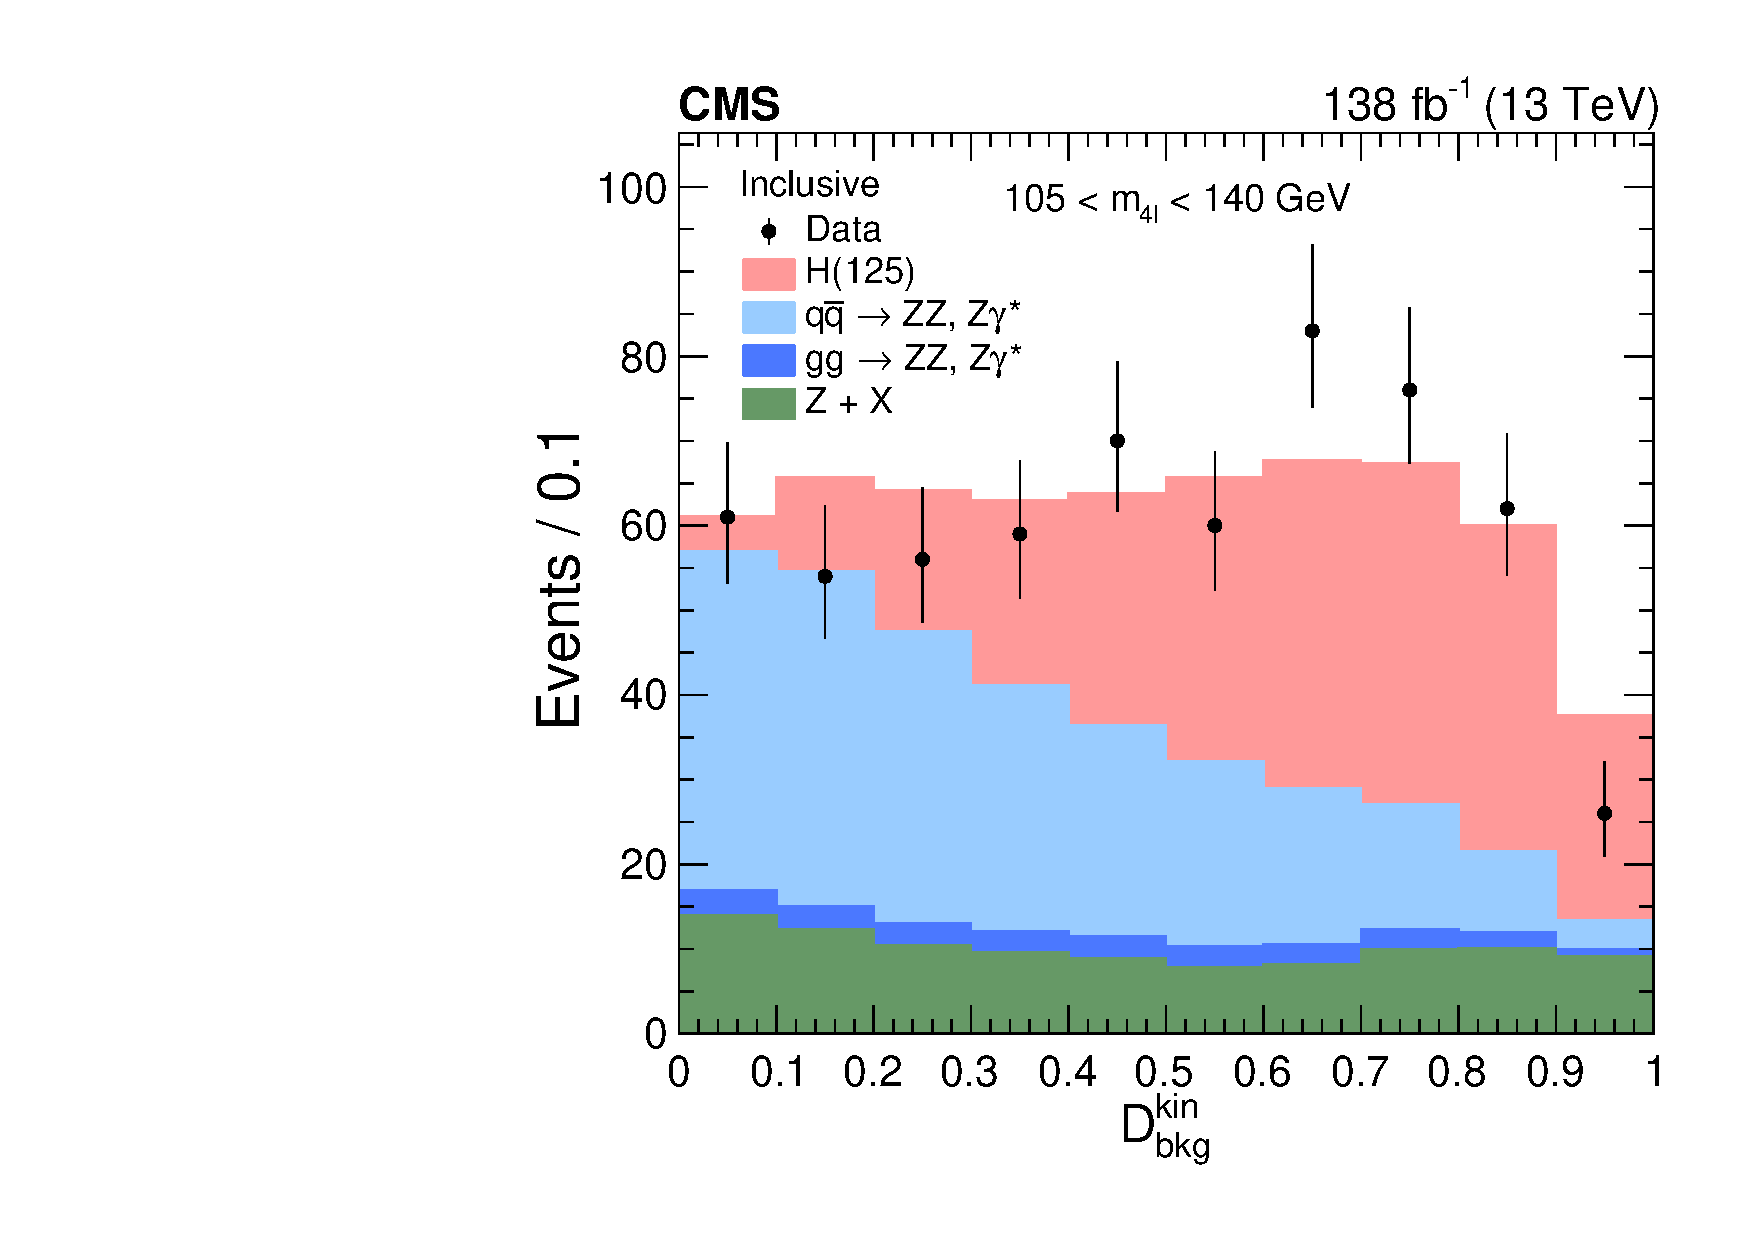
\includegraphics[width=0.8\textwidth,clip] {figures/Figure_004.pdf}
\caption{Distributions of the observed (points) and predicted (stacked histograms) \Dbkgkin of the four-lepton system, in the inclusive final state. The predictions for the \Hboson signal and the three main backgrounds are given by the different colors.  The vertical bars on the points show the statistical uncertainties in the data.}
\label{fig:DiscDist}
\end{figure}

% \begin{figure}[!htb]
% \centering
% 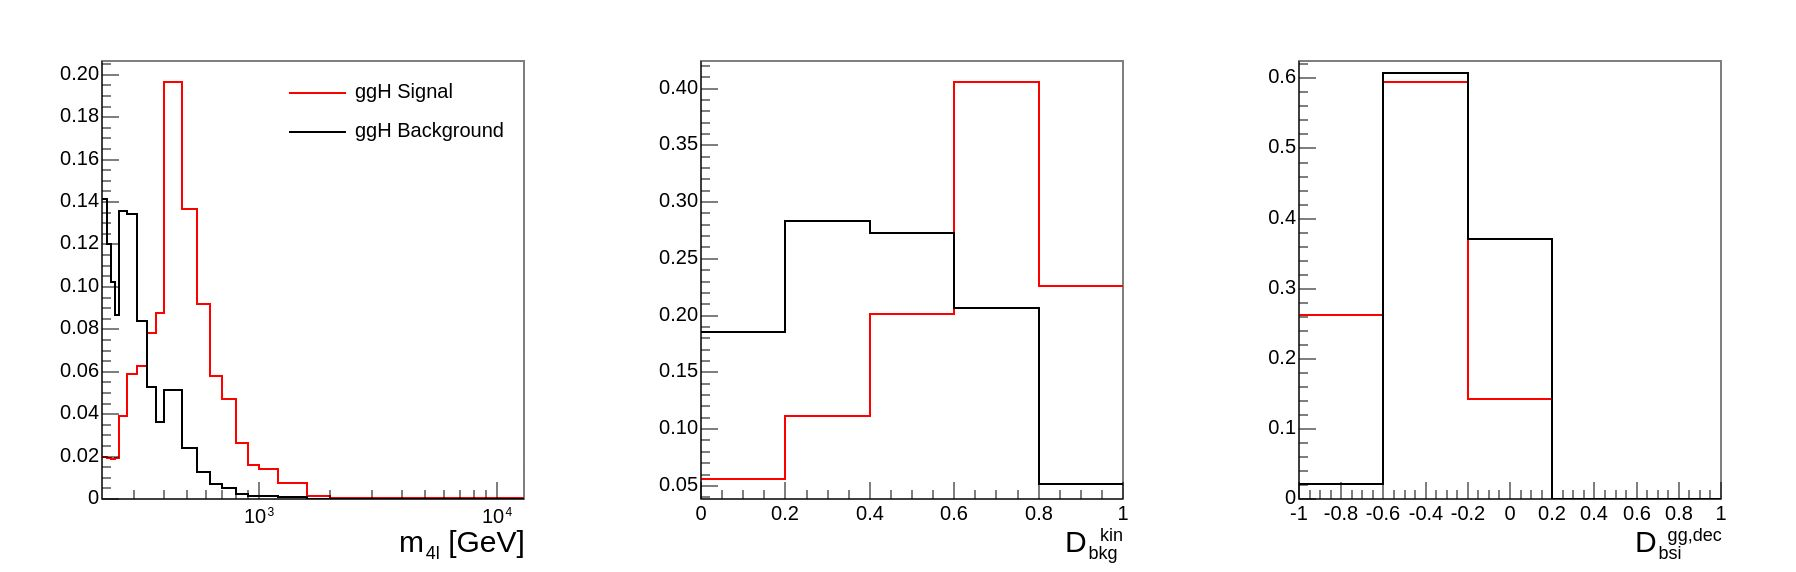
\includegraphics[width=0.8\textwidth,clip] {figures/DiscDists.jpg}
% \caption{}
% \label{fig:DiscDists}
% \end{figure}

The gluon fusion cross section is computed utilizing the highest-order QCD and electroweak (EW) expansions available for inclusive $ZZ$ production~\cite{deFlorian:2016spz}. 
However, event categorization relies on the modeling of associated jets through PYTHIA's parton showering and hadronization algorithms, which necessitates proper matching to the underlying hard-scattering process. Off-shell gluon fusion production is generated at leading order (LO) without associated jets at the matrix element level, implying that all reconstructed jets originate from PYTHIA's modeling. 
The parton showering and hadronization processes require specification of the hadronization scale, which is typically dependent on the characteristic energy scale of the process—set to $m_{4\ell}$ in the case of $gg\to 4\ell$.

For EW production mechanisms, the inclusive production cross section of $ZZ$ with two associated jets is similarly calculated using the highest-order QCD and EW expansions available~\cite{deFlorian:2016spz}. 
In contrast to gluon fusion, two hard jets—typically the leading jets in the event—are generated intrinsically at the matrix element level in the LO simulation. 
These jets correspond to either the forward-backward jets characteristic of vector boson fusion (VBF), or to the hadronic decay products of an associated W or Z boson. 
Consequently, the dependence on PYTHIA's parton shower and hadronization algorithms, and their matching to the hard-scattering production, is substantially reduced for these EW processes.

The categorization efficiency for simulated ggH and EW \Hboson production can be validated through comparison with alternative POWHEG and MINLO simulations. 
The POWHEG samples are generated across a broad range of off-shell \Hboson masses at next-to-leading order (NLO) in QCD, with one jet generated at the matrix element level and additional jets simulated through PYTHIA matching. 
The MINLO simulation of ggH production is performed for \Hboson masses of 125 and $300$ GeV at NLO in QCD, with two jets generated at the matrix element level and additional jets modeled via PYTHIA matching.

While JHUGen categorization efficiencies are consistent with those from POWHEG and MINLO within the uncertainties associated with the QCD scale implementation in PYTHIA,
the ggH process exhibits deviations in central values and corresponding uncertainties of up to 20\% in the signal-dominated $m_{4\ell}$ range of 300--500 GeV, with category-dependent variations. 
For EW processes, categorization efficiencies typically agree within 5--10\% between methodologies. 
We implement a correction procedure whereby the categorization efficiency as a function of $m_{4\ell}$ is adjusted to match that of the SM signal derived from POWHEG samples, with the assumption that this correction applies equally to background and interference contributions. 
This procedure ensures conservation of the total event yield across all three categories at each $m_{4\ell}$ value. An illustration of these categorization corrections can be found in Figure~\ref{fig:ew_catcor}.

\begin{figure*}[h!]
\centering
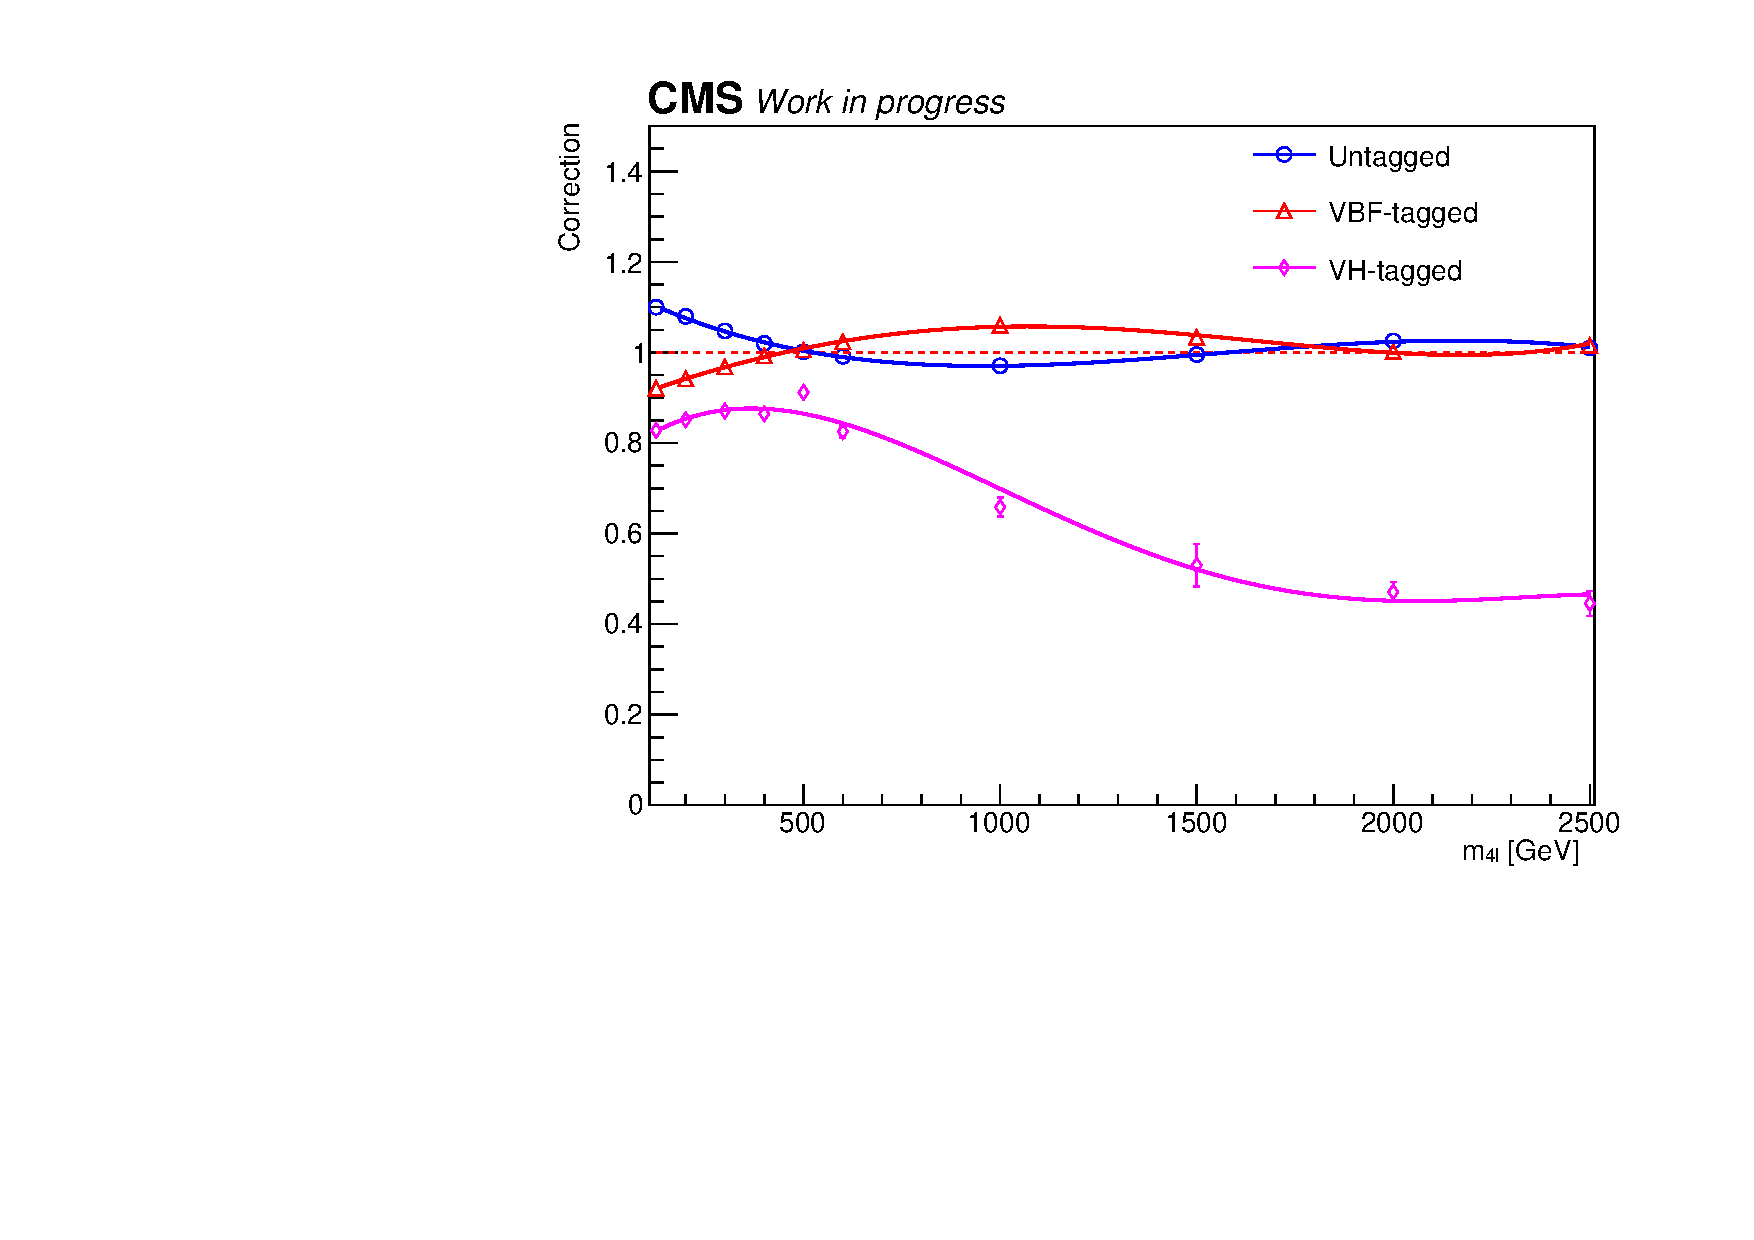
\includegraphics[width=0.85\textwidth]{figures/Corrections_allyears.pdf}
\caption {
Corrections as a function of $m_{4\ell}$ for \offshell EW process selection efficiencies in the Untagged, VBF-tagged, and VH-tagged categories. A polynomial fit is performed extending up to $2.5$ TeV. Events with $m_{4\ell}$ $ >  2.5$ TeV assume the correction value at the $2.5$ TeV cut-off. The correction is shown for the three data-taking periods in Run 2 combined.
\label{fig:ew_catcor}}
\end{figure*}

The simulation of the $\vec{x}$ observables enumerated in Table~\ref{tab:categoriesoffshell} remains unaffected by jet modeling in the Untagged category. Furthermore, the modeling of observables in jet-tagged categories for EW processes demonstrates remarkable consistency between direct MCFM+JHUGen samples and reweighted POWHEG+JHUGen implementations. 
However, jet modeling in jet-tagged categories for the ggH process significantly impacts the parametrization of probability distributions. Therefore, within these two jet-tagged categories, the gluon fusion process is implemented through reweighted POWHEG+JHUGen simulation, which provides more precise parton shower matching and consequently superior modeling of associated jet activity. In this framework, samples are reweighted according to the appropriate theoretical model using the MELA package.

The observed and expected distributions of observables $\vec{x}$ for events in the \offshell region are illustrated in Figure~\ref{fig:ObservablesCat} for each of the three categories. The expected distributions are found using the SM predicted signal and background cross sections.

\begin{figure*}[!htb]
\centering
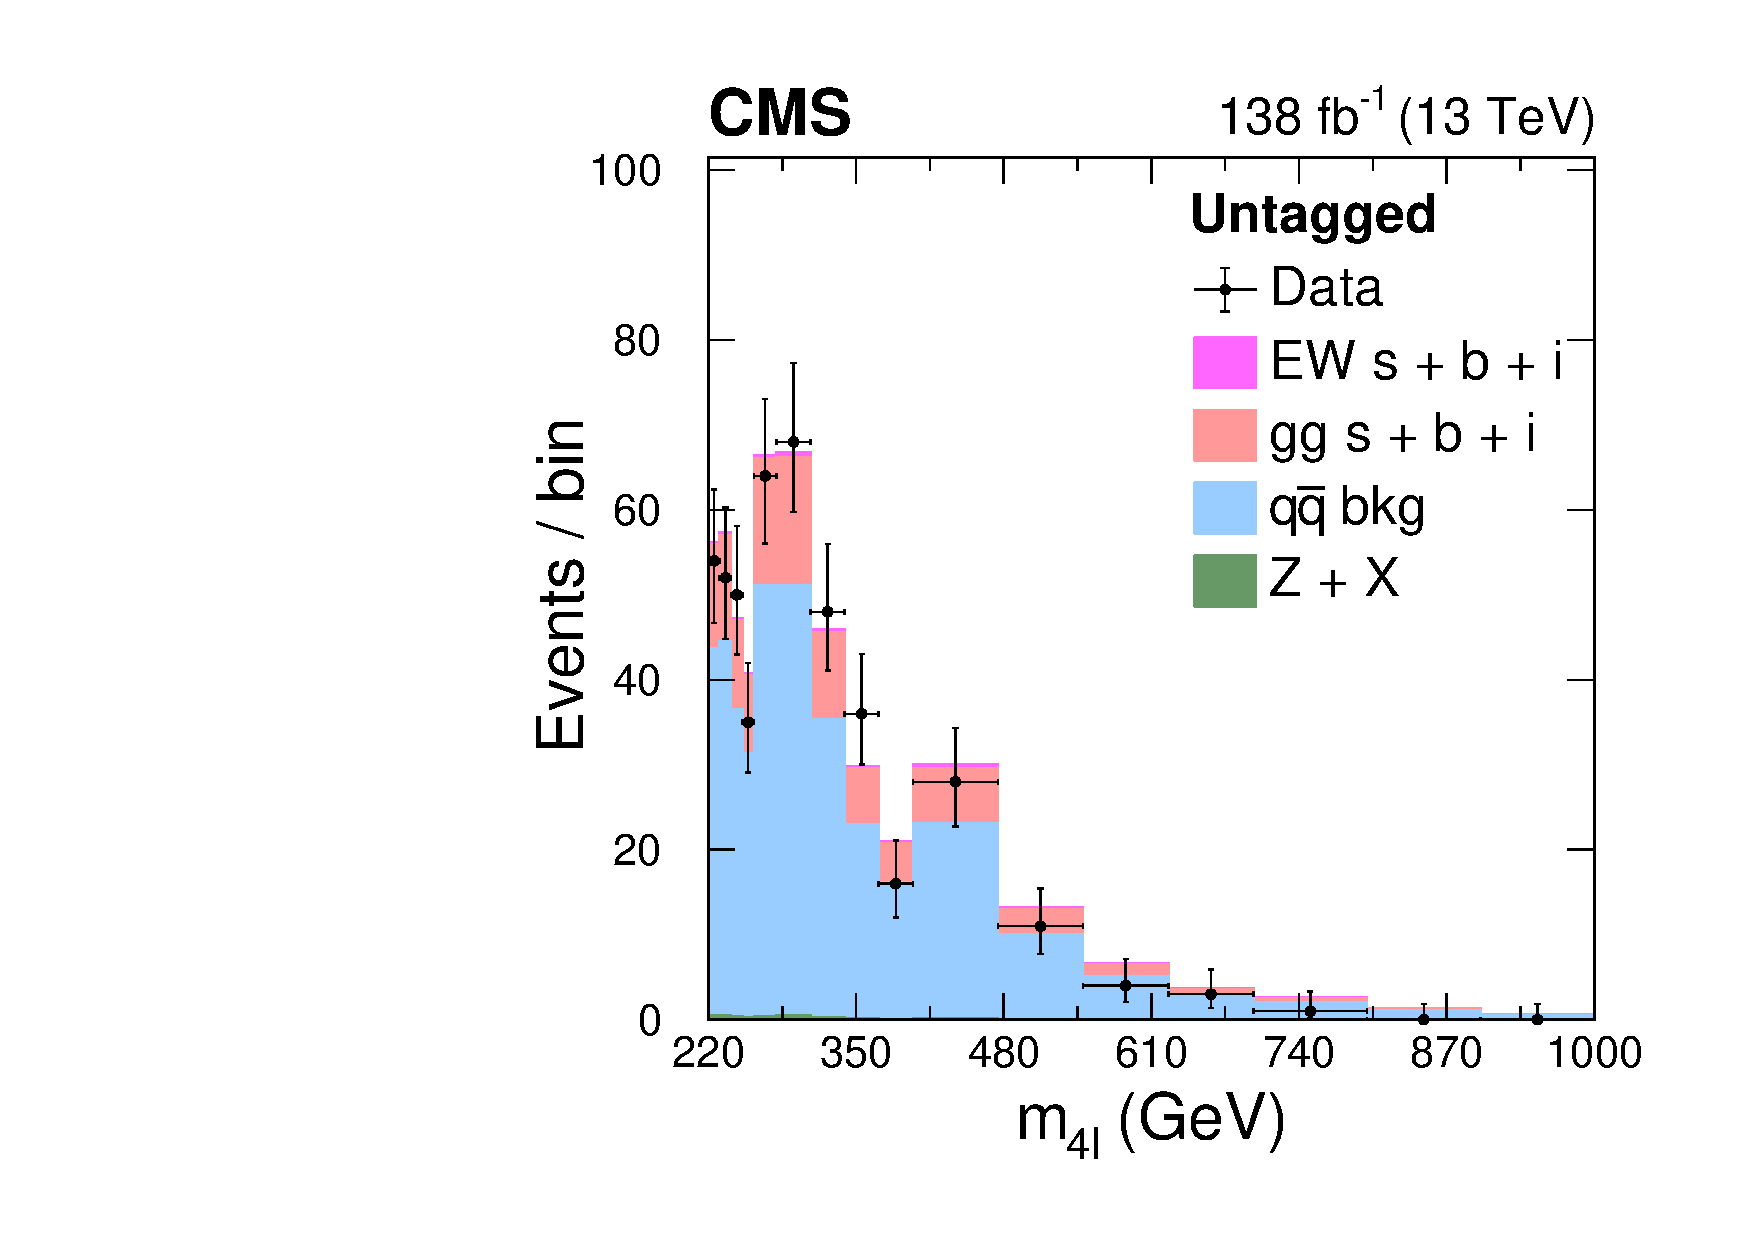
\includegraphics[width=0.31\textwidth]{figures/Figure_005-a.pdf}
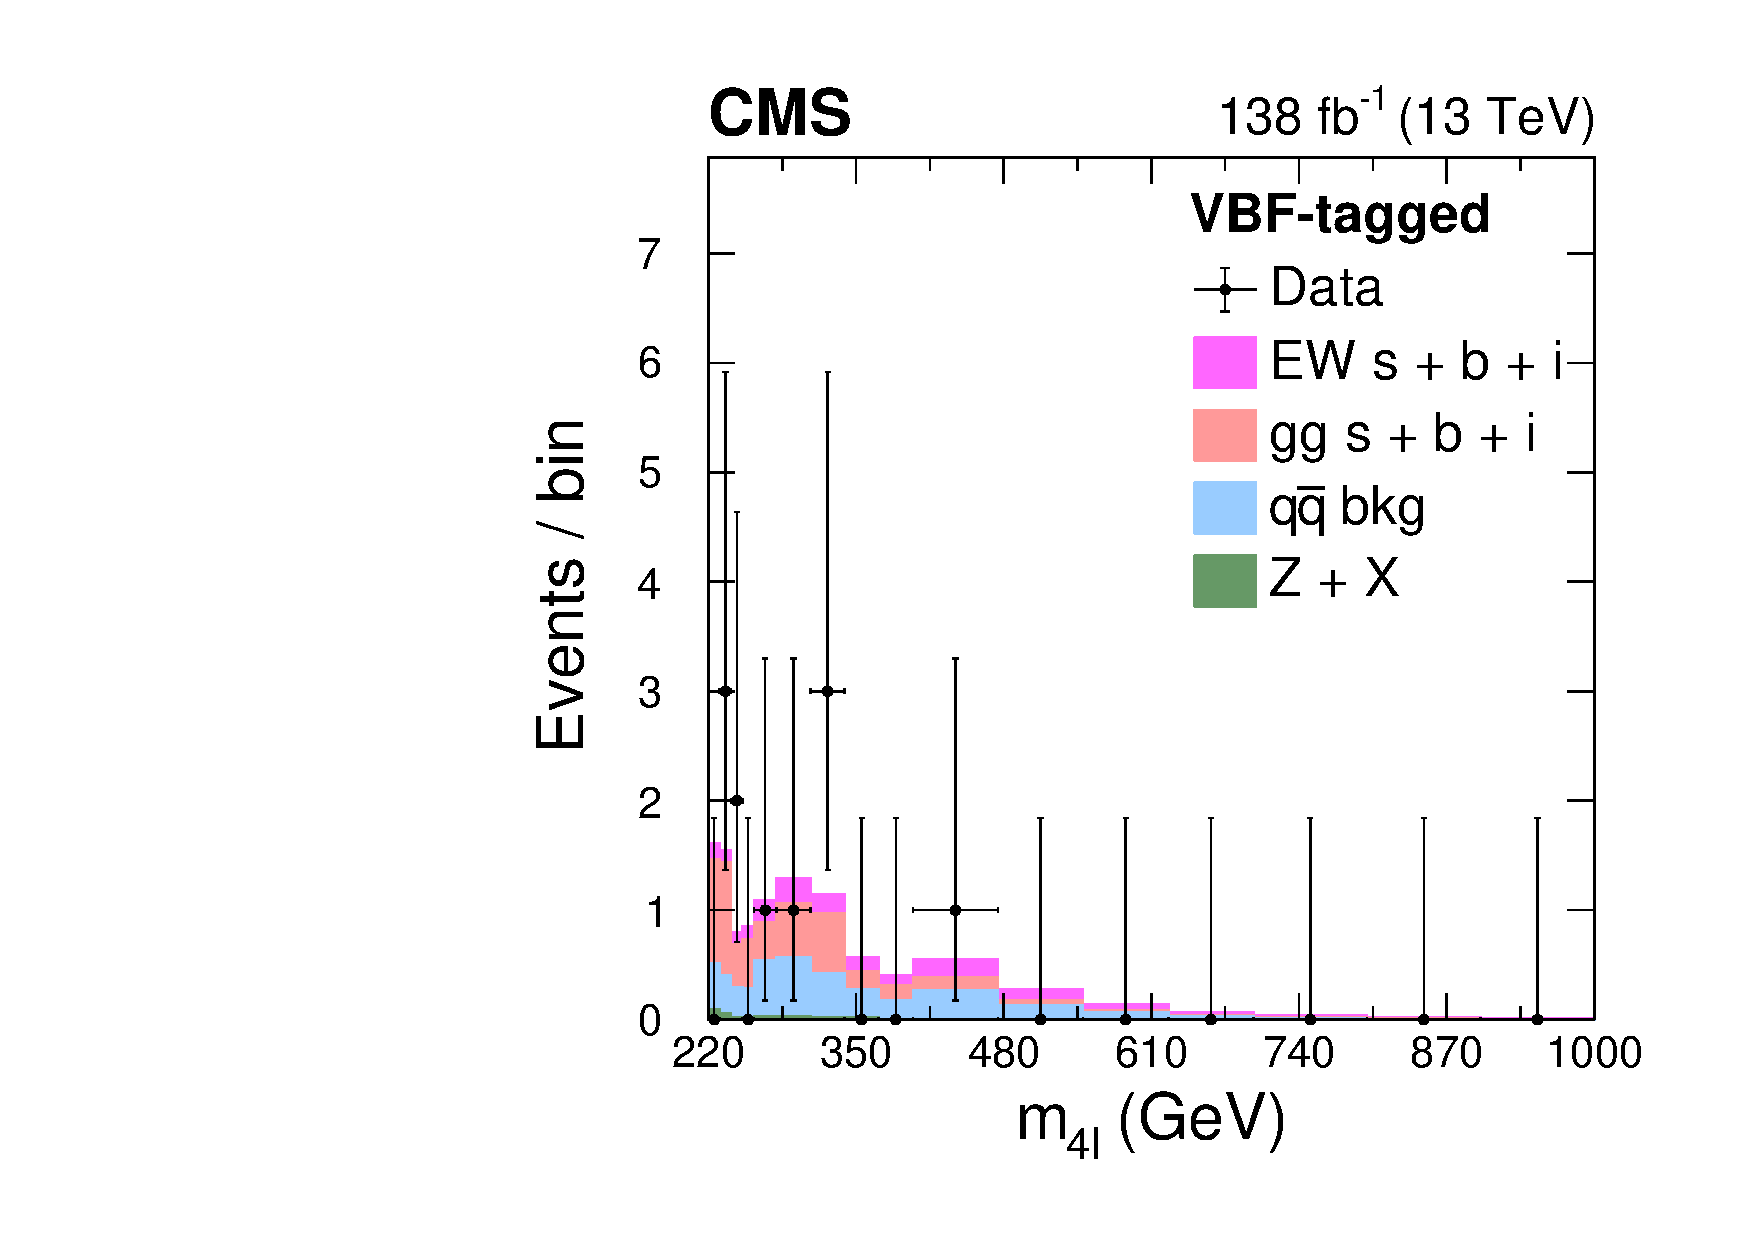
\includegraphics[width=0.31\textwidth]{figures/Figure_005-b.pdf}
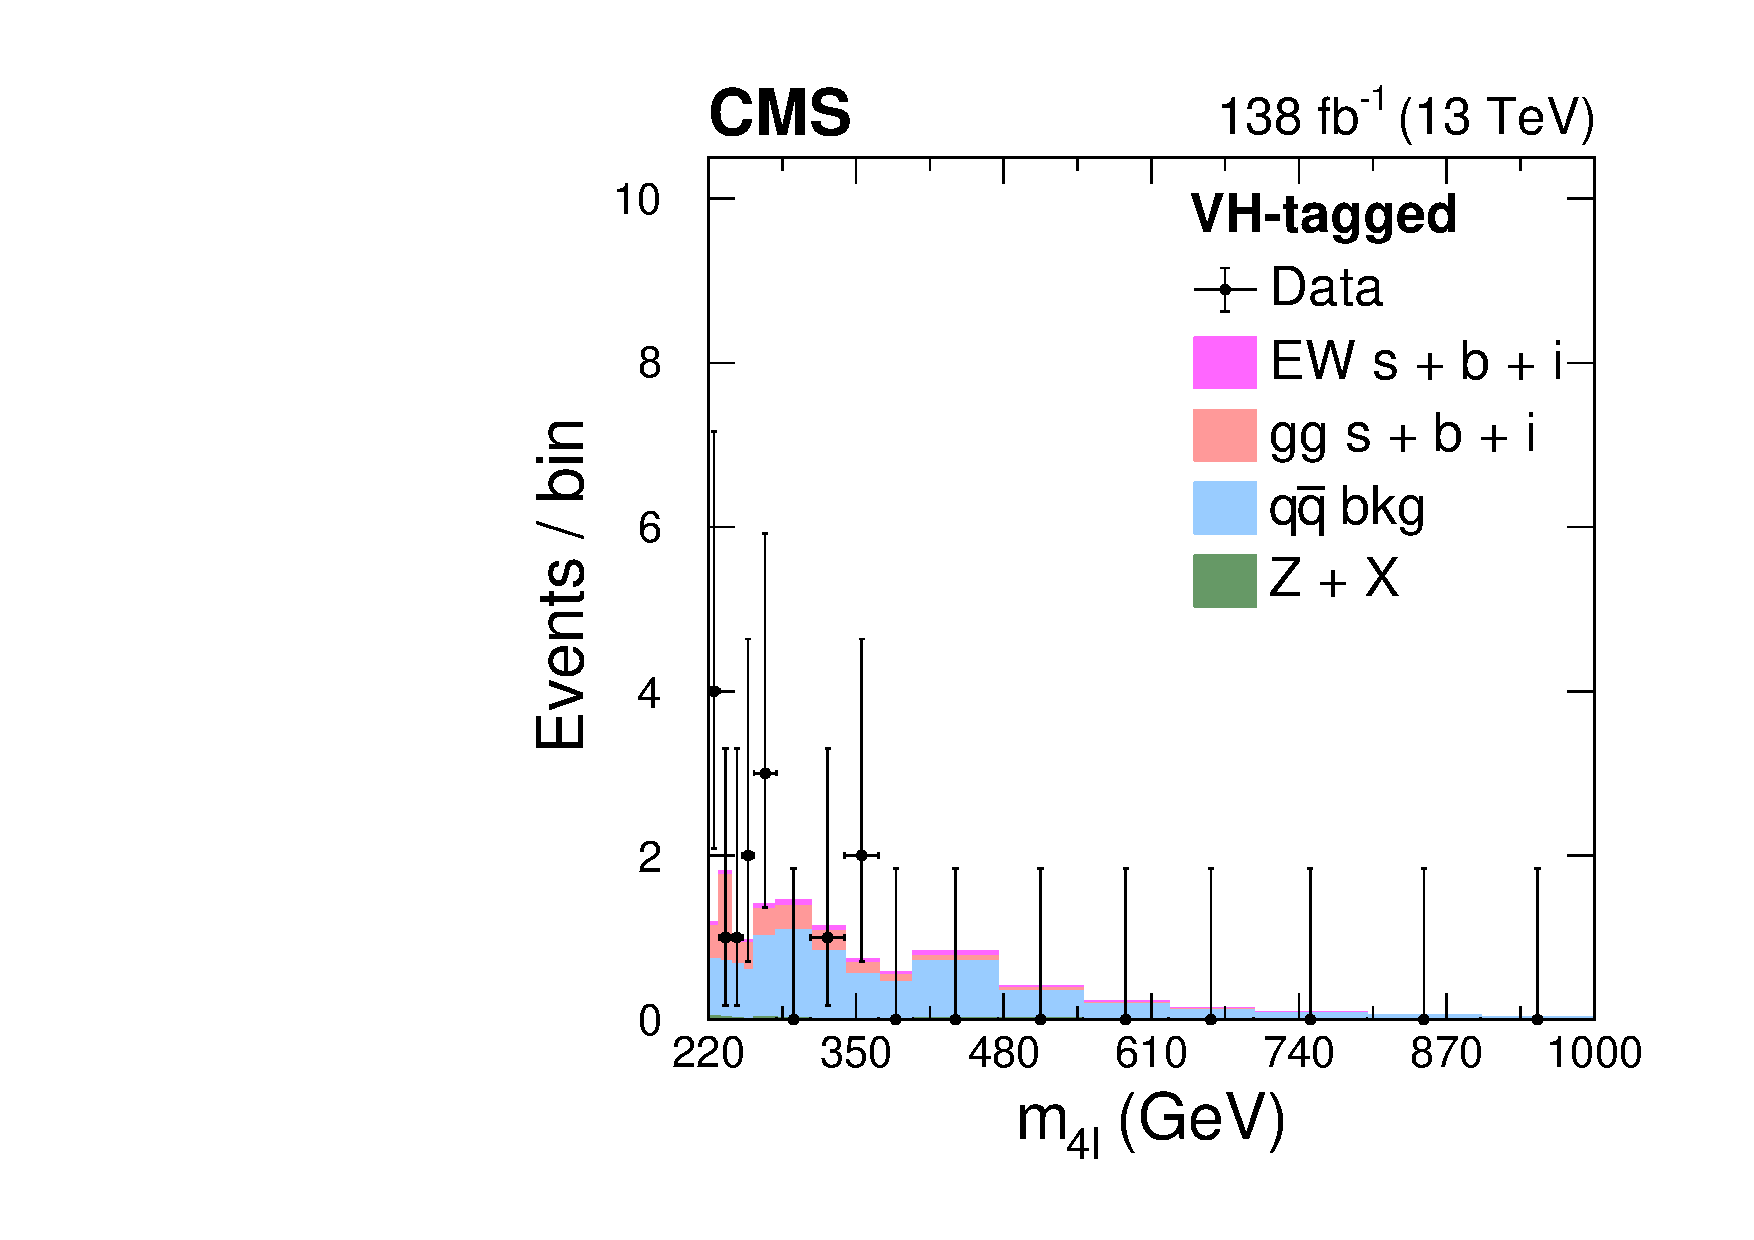
\includegraphics[width=0.31\textwidth]{figures/Figure_005-c.pdf}\\ 
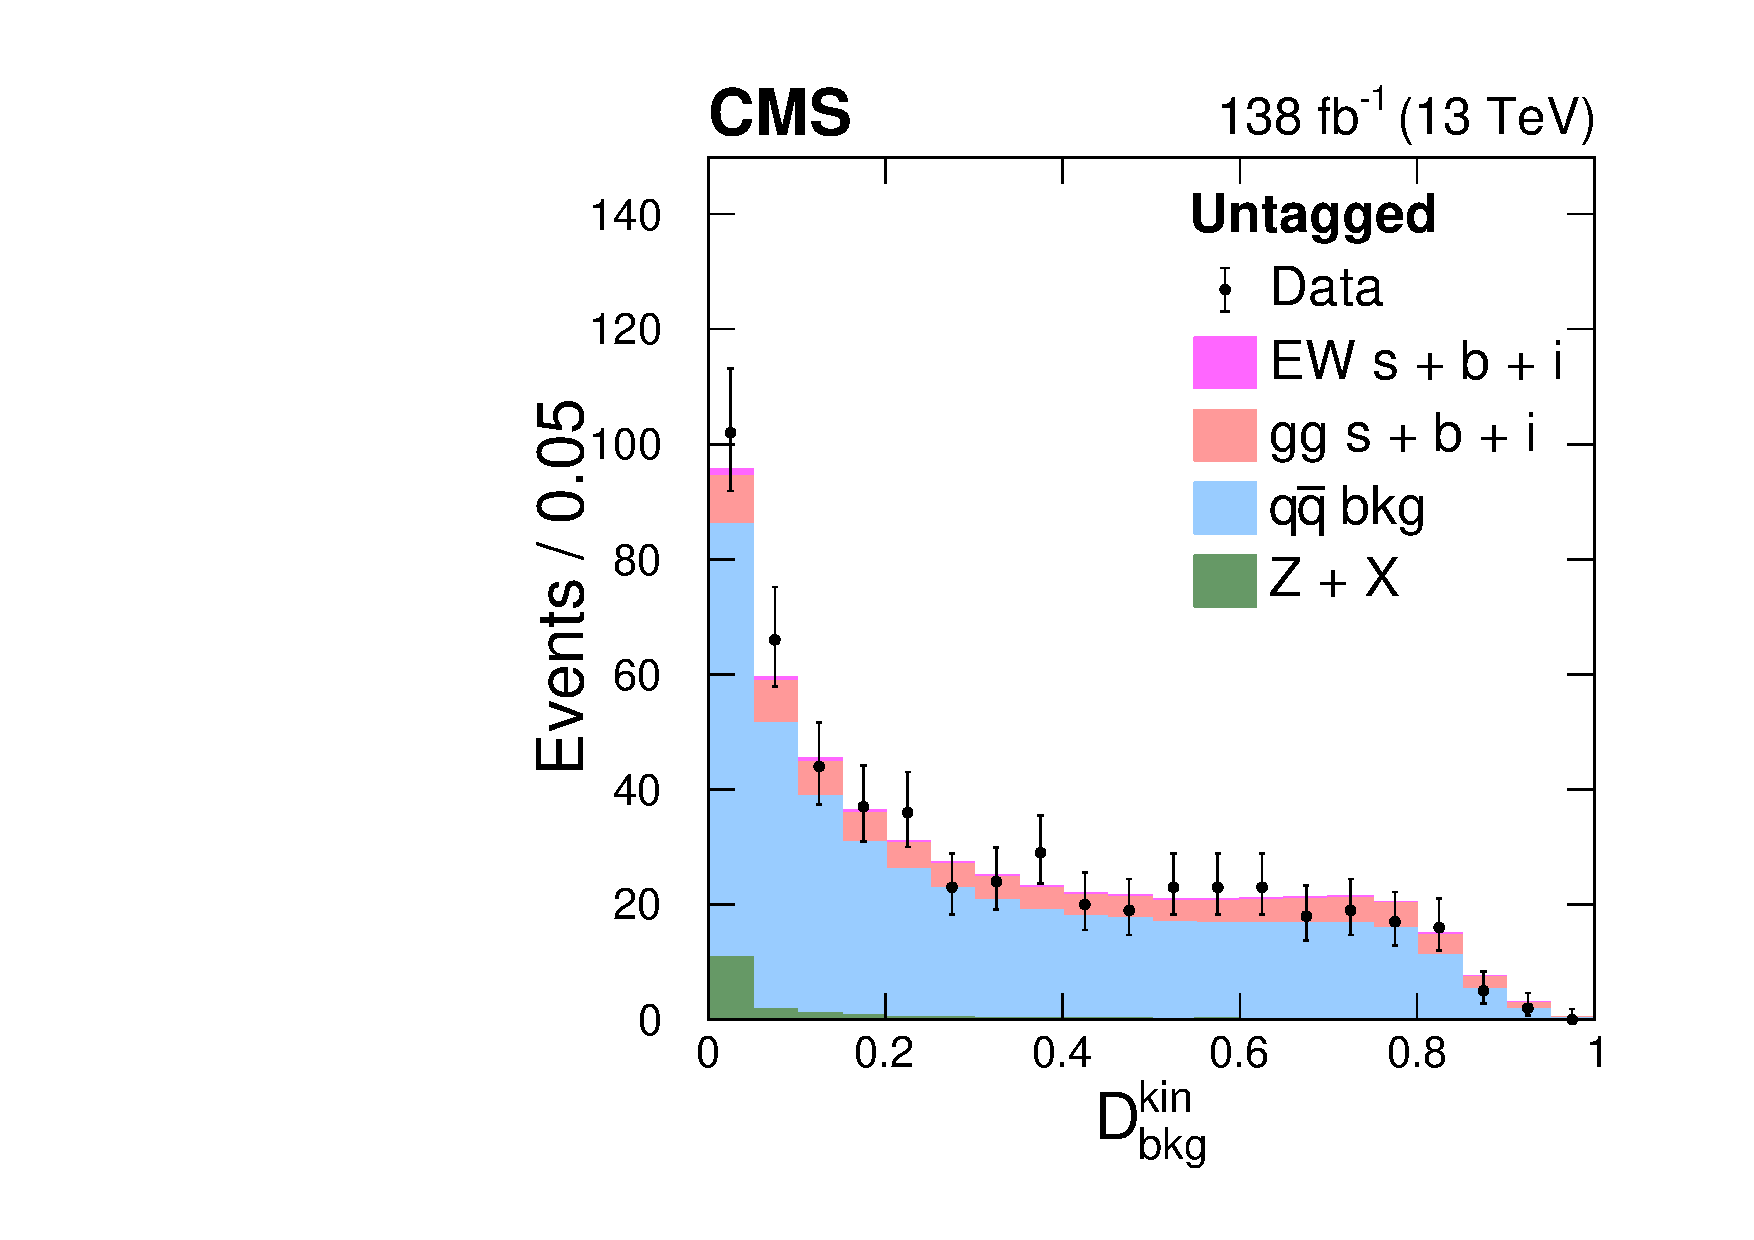
\includegraphics[width=0.31\textwidth]{figures/Figure_005-d.pdf}
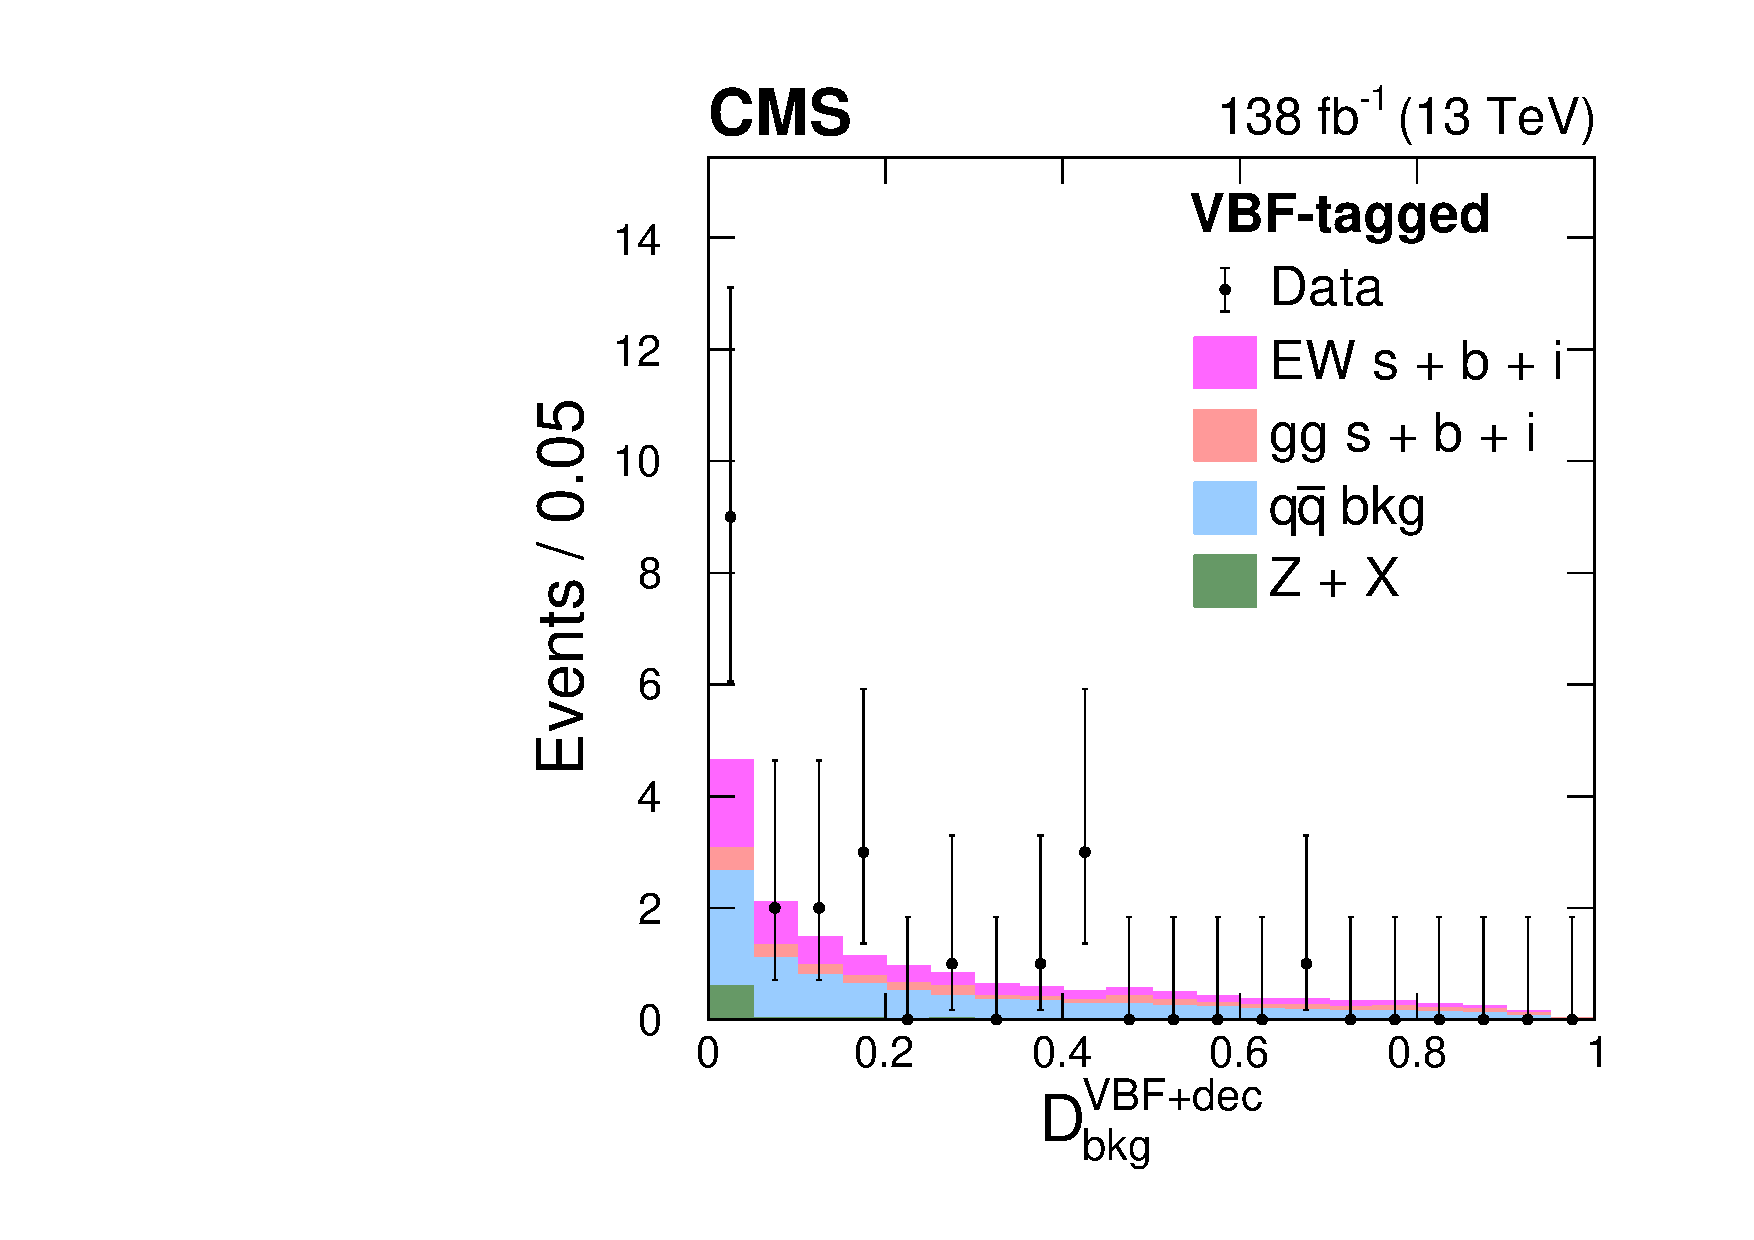
\includegraphics[width=0.31\textwidth]{figures/Figure_005-e.pdf} 
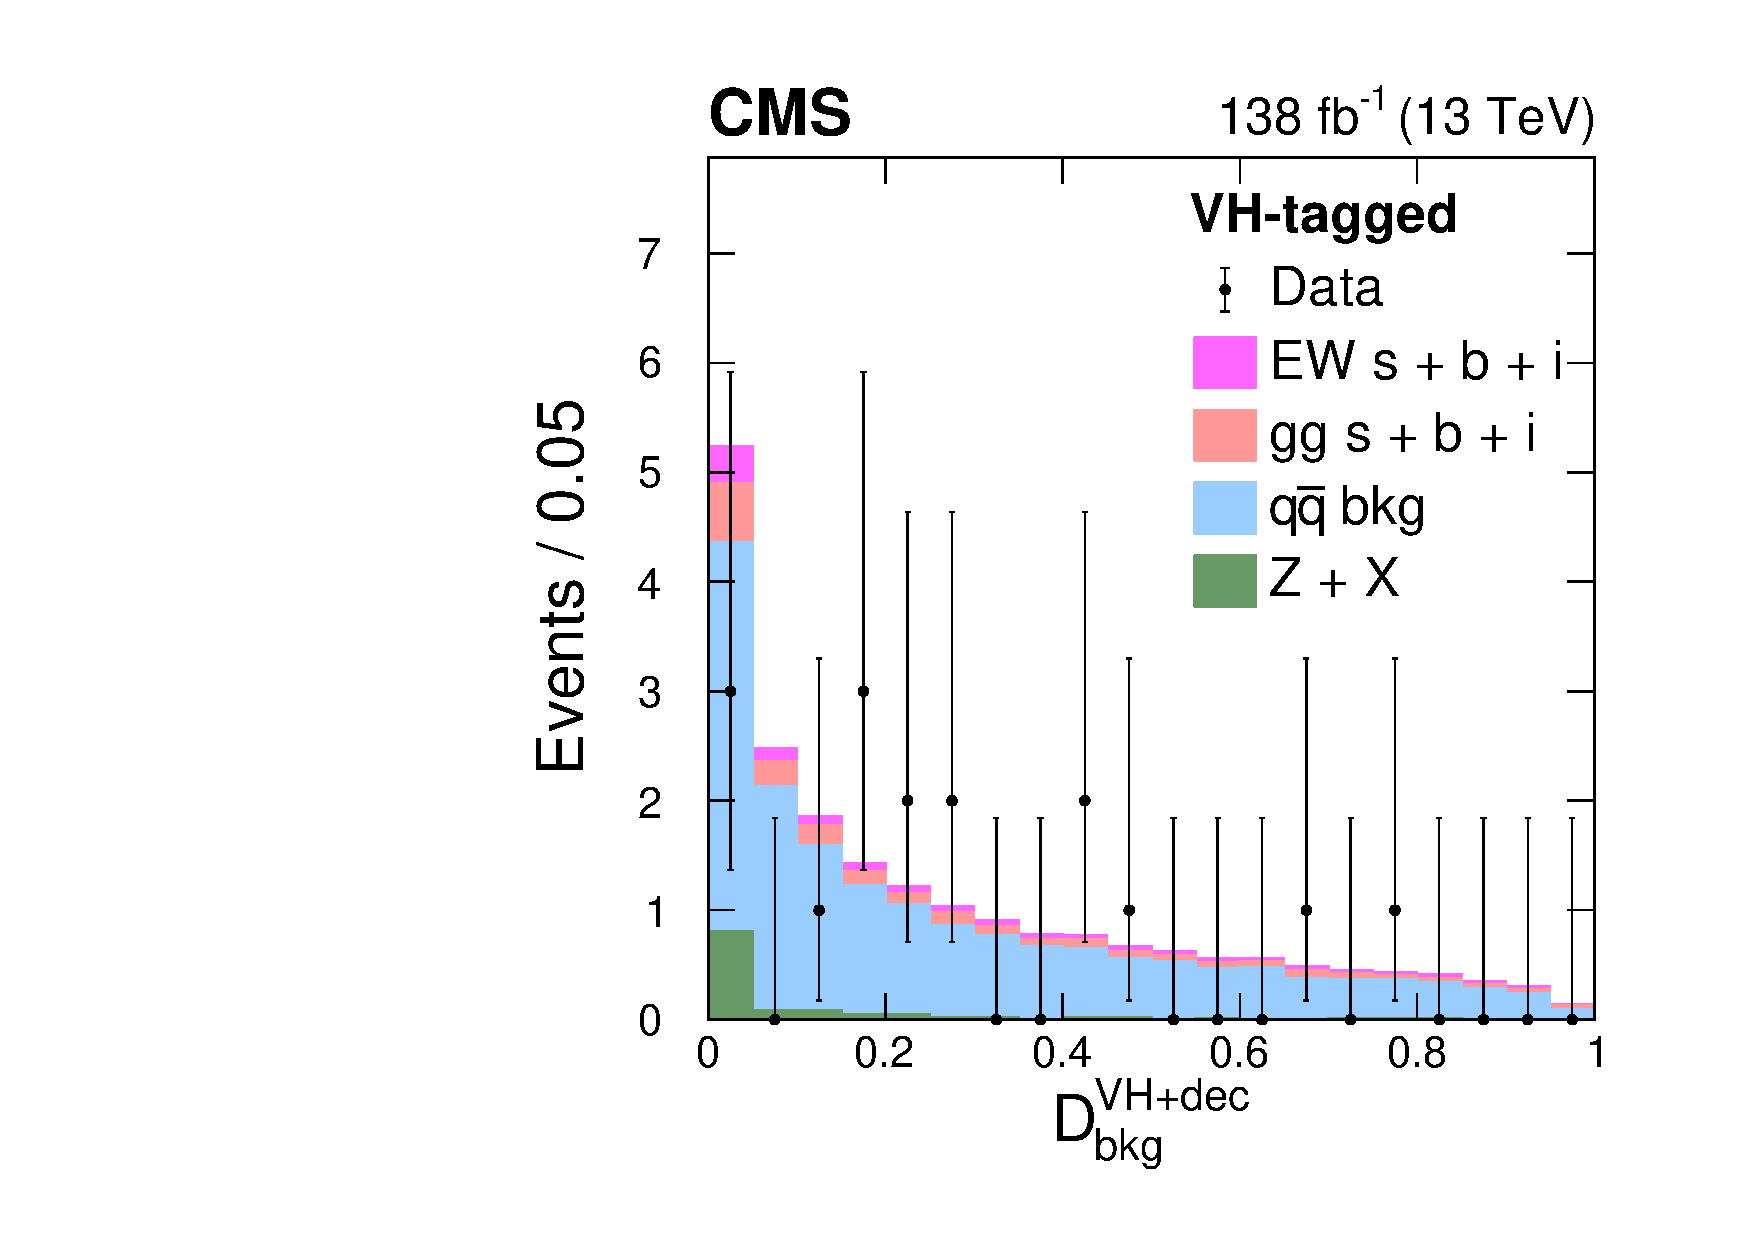
\includegraphics[width=0.31\textwidth]{figures/Figure_005-f.pdf}\\ 
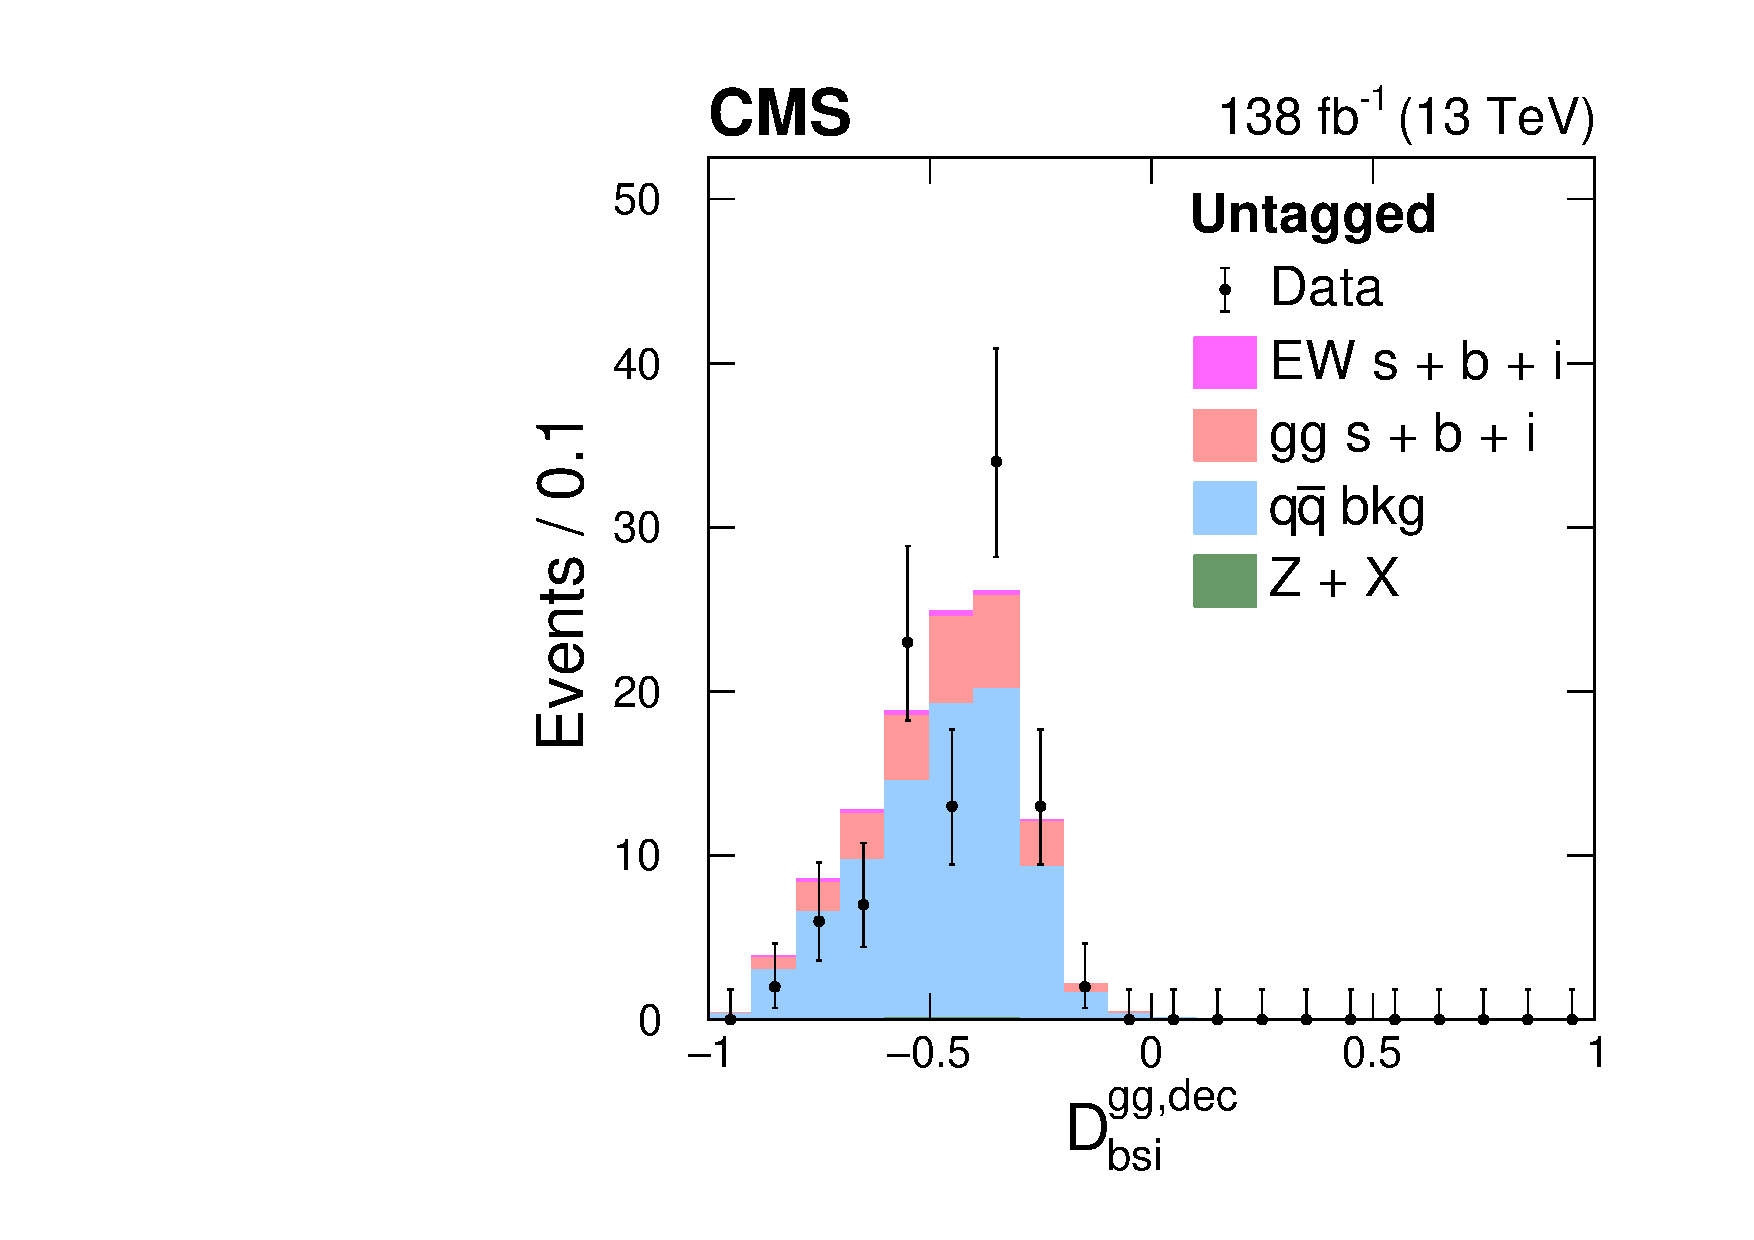
\includegraphics[width=0.31\textwidth]{figures/Figure_005-g.pdf}
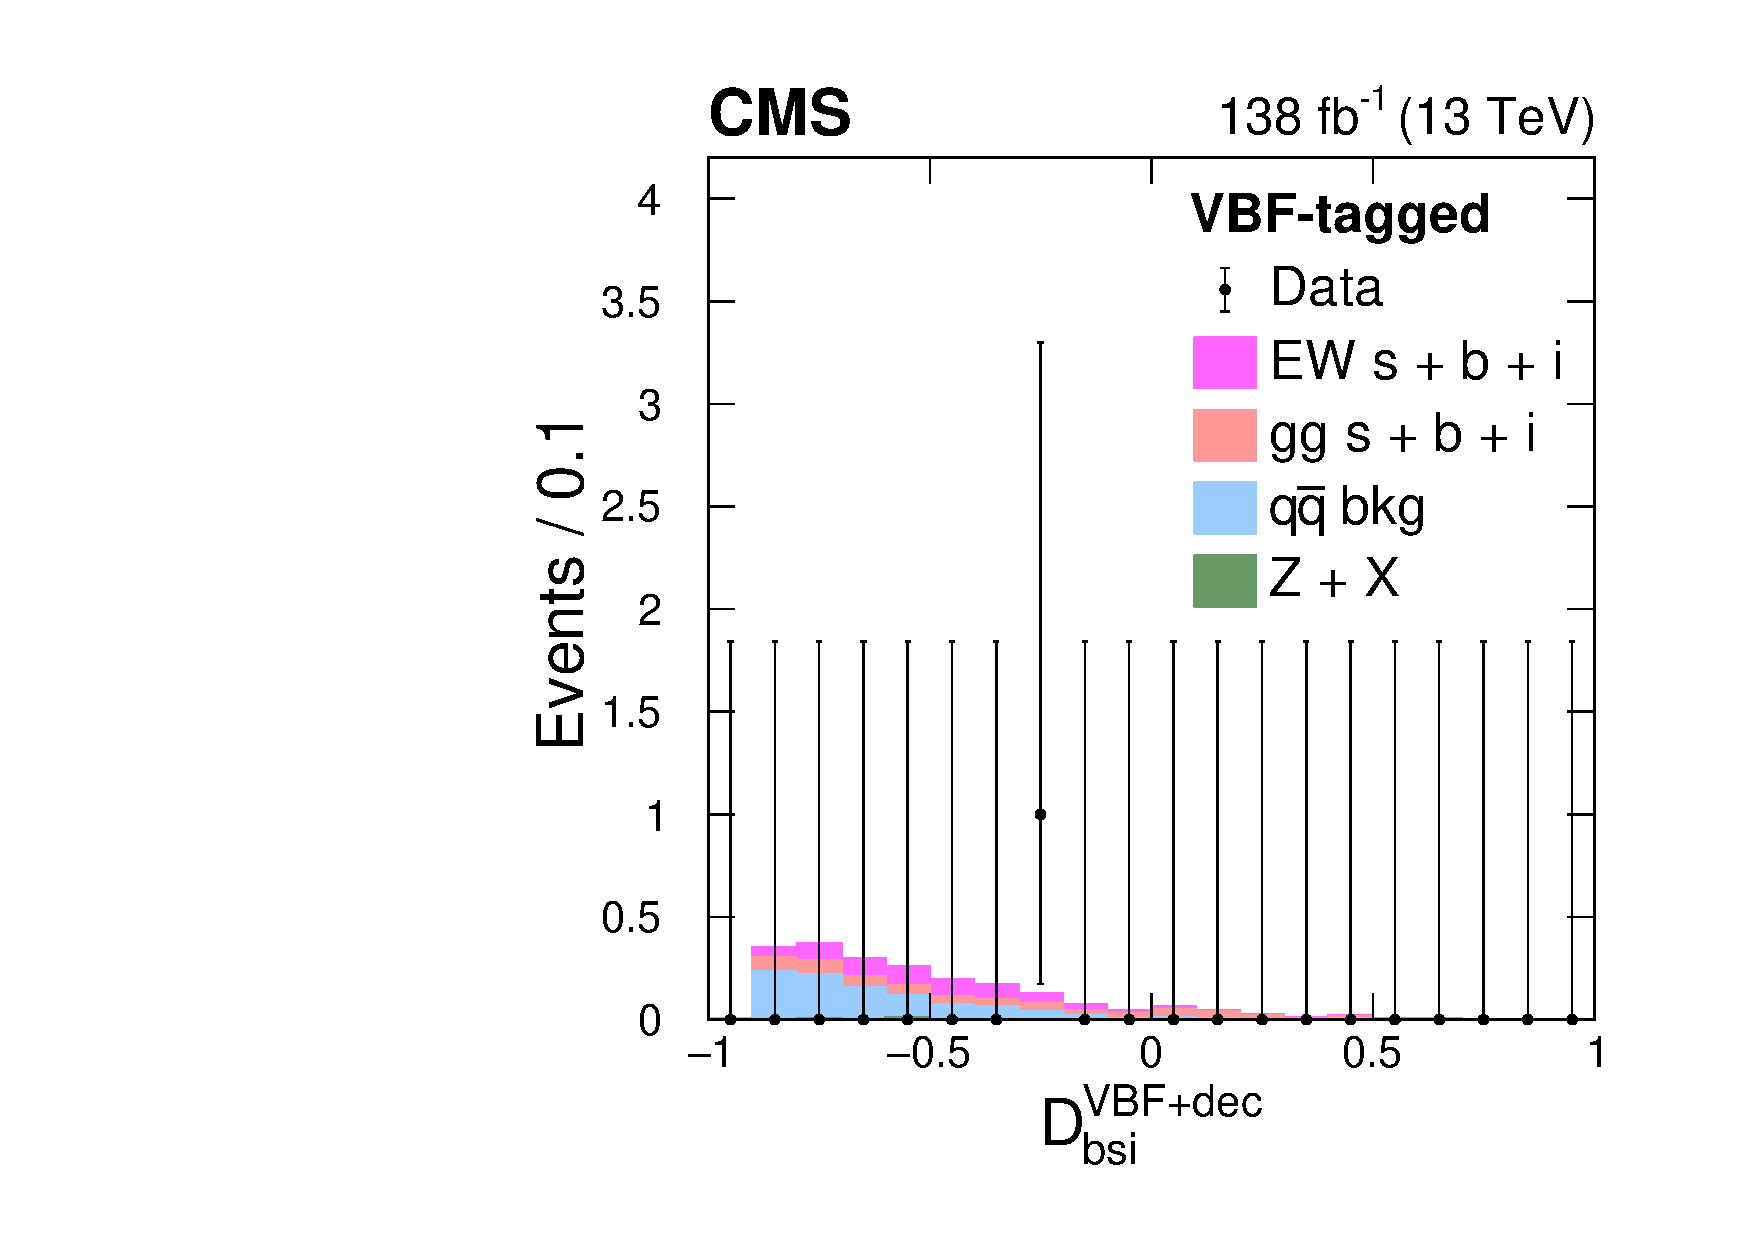
\includegraphics[width=0.31\textwidth]{figures/Figure_005-h.pdf} 
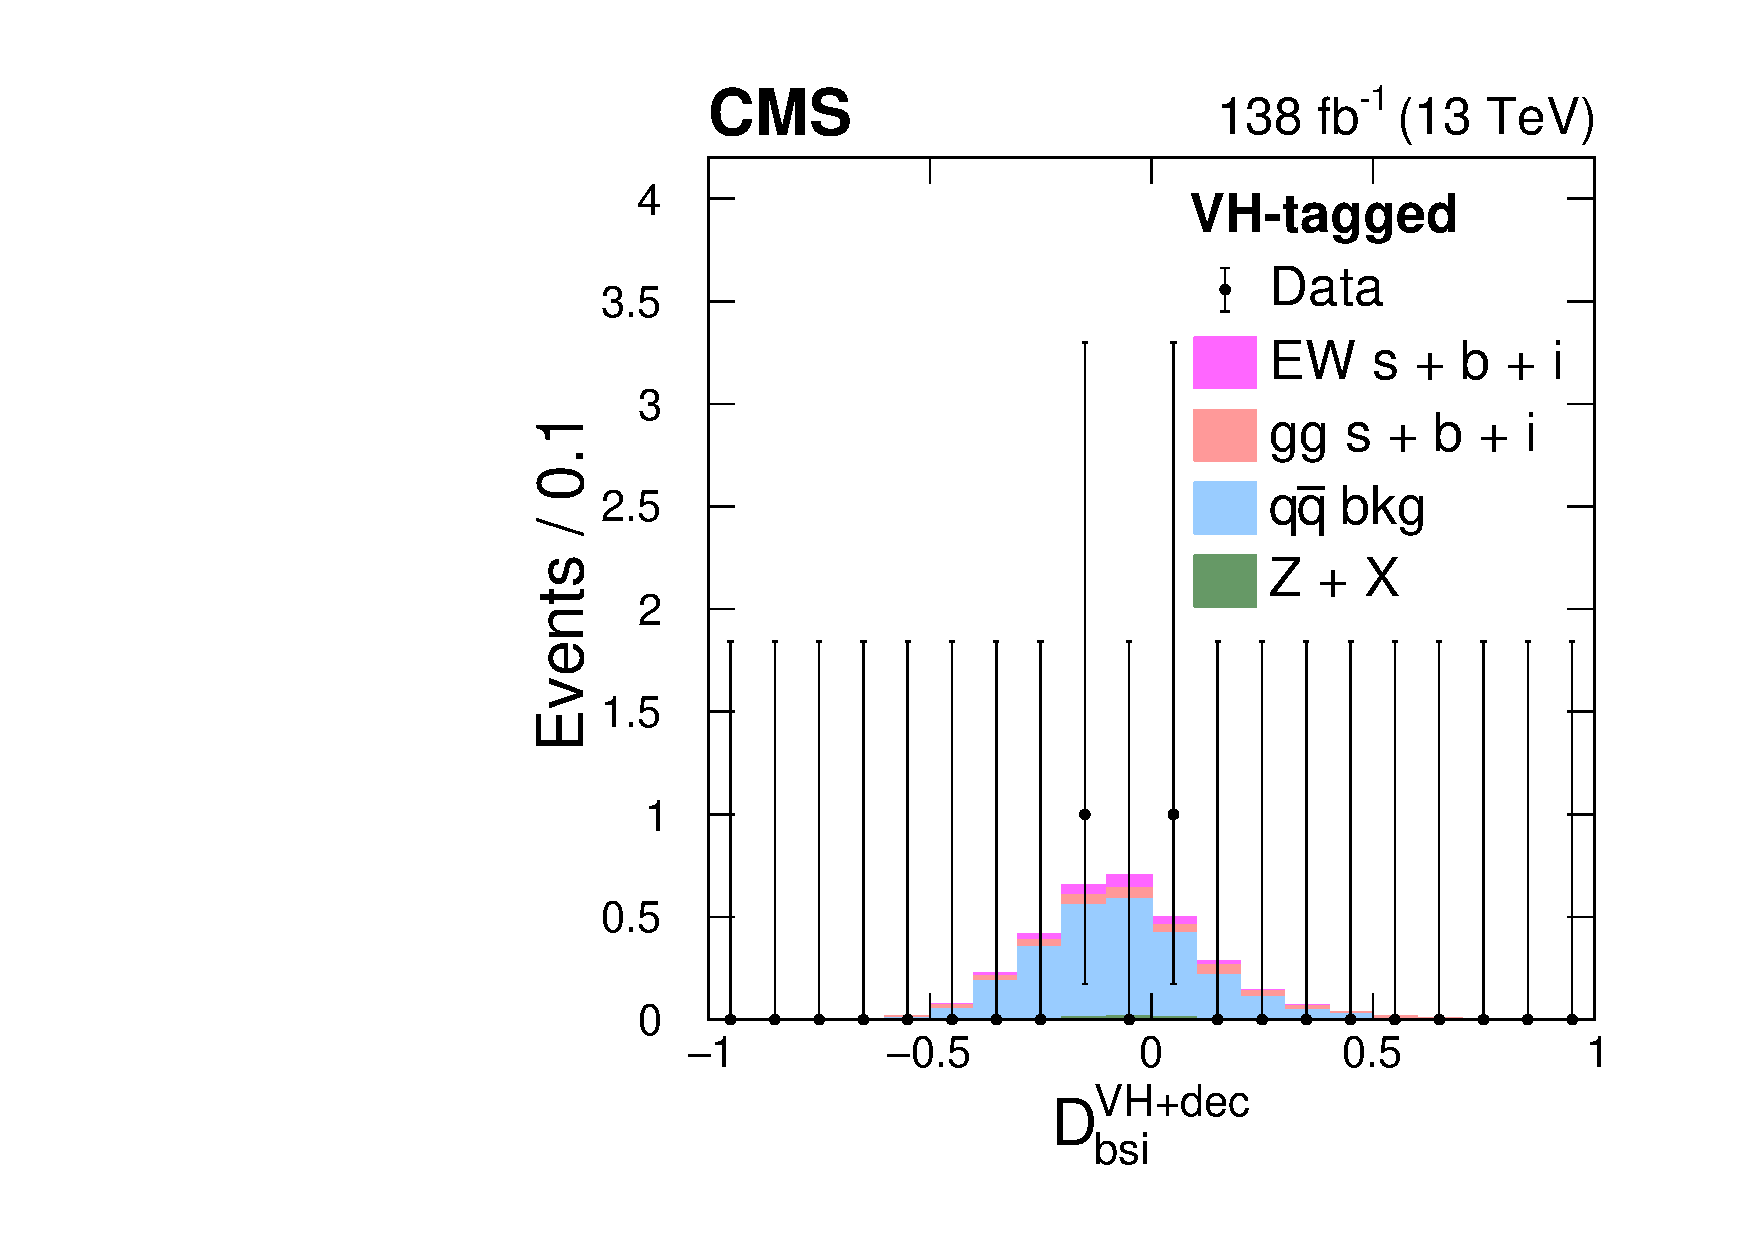
\includegraphics[width=0.31\textwidth]{figures/Figure_005-i.pdf}\\ 
\caption{
Off-shell data (points) and pre-fit distributions (histograms) for the Untagged (left), VBF-tagged (middle), and VH-tagged (right) categories.
The upper row shows $m_{4\ell}$ distributions with a requirement on $\Dbkgkin>0.6$ (left), 
$\mathcal{D}^{{VBF}+{\text{dec}}}_\text{bkg}>0.6$ (middle), or $\mathcal{D}^{{VH}+{\text{dec}}}_\text{bkg}>0.6$ (right)
applied for illustration purposes to enhance signal over background contributions.
The middle row shows $\mathcal{D}^\text{kin}_\text{bkg}$ (left), $\mathcal{D}^{{VBF}+{\text{dec}}}_\text{bkg}$ (middle), $\mathcal{D}^{{VH}+{\text{dec}}}_\text{bkg}$ (right) distributions,
where an additional requirement $m_{4\ell}>340$ GeV is applied to enhance signal-over-background contributions.
The lower row plots the $\mathcal{D}_\text{bsi}$ with both the $m_{4\ell}$ and \Dbkgkin requirements specified above.
Contributions from the four processes are shown by the different colors, where ``s'', ``b'', and ``i'' refer to the 
signal, background, and interference contributions, respectively.
The vertical bars on the points give the statistical uncertainties in the data, and the horizontal bars represent the bin widths. 
For the pre-fit distributions, the different cross sections are set to their SM values~\cite{PhysRevD.111.092014}.
}
\label{fig:ObservablesCat}
\end{figure*}



% The gluon fusion cross section is calculated using the highest order QCD and EW expansions available 
% to simulate inclusive $ZZ$ production~\cite{deFlorian:2016spz}.
% However, event categorization depends on modeling associated jets through PYTHIA's parton showering and hadronization, 
% which involves matching these processes to the hard-scattering production. Off-shell gluon fusion production is generated at LO 
% with no associated jets at the matrix element level, and therefore all jets come from PYTHIA. 
% The parton showering and hadronization requires setting the hadronization scale, which can depend on the energy scale 
% in the process. In the case of the $gg\to 4\ell$ process, the energy scale is set at $m_{4\ell}$.

% The EW cross section for the inclusive production of $ZZ$ and two associated jets is also calculated to the highest order 
% QCD and EW expansion available~\cite{deFlorian:2016spz}. 
% Contrary to the gluon fusion process, two hard jets, which are typically the leading 
% jets in the process, are already generated at the matrix element level in the LO simulation. 
% These are the two associated jets in the VBF process, or 
% the two jets from the hadronic decay of the associated W or Z boson. 
% Therefore, the dependence on the PYTHIA parton shower and hadronization 
% and its matching to the hard-scattering production is much weaker for these EW processes. 

% The categorization efficiency of simulated ggH and EW \Hboson production can be checked using alternative POWHEG and MINLO simulations. 
% The POWHEG samples are generated for a wide range of off-shell \Hboson masses at NLO in QCD, 
% with one jet generated at the matrix element, and using PYTHIA matching to simulate additional jets. 
% The MINLO simulation of ggH production is done for \Hboson masses of 125 and $300$ GeV at NLO in QCD, 
% with two jets generated at the matrix element level, and PYTHIA matching for additional jets.
% While the JHUGen categorization efficiencies agree with those using POWHEG and MINLO 
% within the uncertainties of the QCD scale used in PYTHIA,
% for the ggH process the deviations of the central values and the corresponding uncertainties 
% are up to 20\% in the signal-dominated $m_{4\ell}$ range 300--500 GeV, depending on the category. 
% In the EW process, categorization efficiencies from the two approaches typically agree within 5--10\%. 
% In all cases, we adjust the categorization efficiency as a function of $m_{4\ell}$ to match that for the SM signal 
% obtained from the POWHEG samples, and assume the same behavior for 
% the background and interference contributions. 
% This correction procedure ensures that the total event yield, summed over the three categories,
% is unchanged at each value of $m_{4\ell}$.

% Simulation of the $\vec{x}$ observables listed in Table~\ref{tab:categoriesoffshell}
% is not affected by the jet modeling in the Untagged category. It is also found that the modeling
% of the observables in the jet-tagged categories is nearly the same in the EW process, when 
% compared between the direct MCFM + JHUGen samples and reweighted POWHEG + JHUGen. 
% However, the modeling of jets in the jet-tagged categories for the ggH process does impact 
% the parametrization of the probability distributions. Therefore, within these two jet-tagged categories, 
% the gluon fusion process is incorporated through the reweighted POWHEG + JHUGen simulation. 
% This approach allows a more precise matching with the parton shower, thereby 
% better describing the associated jet activity. In this case, the samples are reweighted for the appropriate 
% model using the MELA package.

\subsection{Modeling of Background}

The largest background in the $H \to 4\ell$ channel originates from the process $q\bar{q} \to ZZ/Z\gamma^*/\gamma^*\gamma^* \to 4\ell$. Additionally, the processes $gg \to ZZ/Z\gamma^*/\gamma^*\gamma^* \to 4\ell$ and electroweak (EW) production---including vector boson scattering and $VZZ$ processes---also contribute to the background and interfere with off-shell \Hboson production. In the \onshell region, this interference is negligible; however, the EW background additionally includes other processes such as $VVV$, $t\bar{t}VV$, and $t\bar{t}V$. To model the invariant mass ($m_{4\ell}$) distribution for each irreducible background component, a third-order Bernstein polynomial is employed over the $m_{4\ell}$ range of 105--140\,GeV~\cite{PhysRevD.111.092014}.

Another important background arises from processes collectively referred to as $Z+X$, where leptons are misidentified from decays of heavy-flavor hadrons, in-flight decays of light mesons within jets, or charged hadrons overlapping with $\pi^0$ decays. The dominant contribution to this background is from $Z$+jets events, estimated using data-driven methods in dedicated control regions. These control regions are defined by selecting events containing one lepton pair meeting the ${Z}_{1}$ candidate requirements, along with an additional pair of opposite-sign leptons passing looser identification criteria compared to the main analysis selection. These four leptons must then satisfy the ${Z}_{1}, {Z}_{2}$ selection criteria. The background yield in the signal region is obtained by weighting the control region events by the lepton misidentification probability ($f_{\ell}$), defined as the probability for a non-prompt lepton to pass the analysis selection. A detailed description of this method can be found in Ref.~\cite{Sirunyan:2017exp}. The $m_{4\ell}$ distribution for the $Z+X$ background is modeled by a Landau function, whose parameters are determined from data over an extended invariant mass range of 70--770\,GeV due to limited event counts.

The observed numbers of data events, expected backgrounds, and signal yields in the on-shell and off-shell regions are summarized in Tables~\ref{table:yields_SR} and \ref{tab:templateyields_offshell}, respectively. The signal and $ZZ$ background yields are derived from simulation, whereas the $Z+X$ background yield is obtained directly from data. Further details on the modeling of the \Hboson signal, interference effects with background processes, and $ZH$ cross-feed in the off-shell analysis are provided in Section~\ref{physicsmodel}.

\begin{table*}[!htb] 
\centering
\begin{tabular}{lrrrrr}
   	&	$4\mu$	&	4e	&	$2e2\mu$	&	$2\mu2e$	& Total \\
\hline
Total signal    &       90.9    &       48.7    &       65.5    &       53.3    &       258.4   \\
$q\bar{q}\to4\ell$ background 	&	89.2	&	38.9	&	64.4	&	42.1	&	234.6	\\
$gg\to4\ell$ background	&	9.7	&	4.9	&	4.9	&	3.8	&	23.4	\\
$Z+X$ background	&	32.4	&	12.2	&	28.2	&	18.6	&	91.3	\\
Total expected	&	222.2	&	104.6	&	163.0	&	117.8	&	607.7	\\	
Observed	&	230	&	94	&	170	& 107	&	601	\\
\end{tabular}
\caption{The observed and expected yields for the \Hboson signal and background contributions in the \onshell region $105<m_{4\ell}<140$ GeV, for each of the four-lepton categories and the total~\cite{PhysRevD.111.092014}.}
\label{table:yields_SR}
\end{table*}

\begin{table*}[!htb] 
\centering
\begin{tabular}{lrrrr}
& VBF-tagged & VH-tagged & Untagged & Total \\
\hline
$gg\to4\ell$ signal &1.0 & 0.9 & 25.1 & 27.0 \\
$gg\to4\ell$ background & 16.0 & 13.5 & 457.0& 486.4 \\
$gg\to4\ell$ interference & $-2.1$ & $-1.9$  &  $-52.0$ & $-56.1$ \\
EW signal         & 1.3 & 0.1 & 1.8& 3.2\\
EW background     & 14.9 & 2.9 & 19.7& 37.5\\
EW interference     & $-3.4$ & $-0.2$ & $-3.9$ & $-7.4$ \\
$ZH$ cross-feed & 0.2 & 0.4 & 7.0& 7.6 \\
$q\bar{q}\to4\ell$ background & 28.6 & 46.7 & 1795.1 & 1870.4  \\
$Z+X$ background & 4.7 & 5.3 & 89.7& 99.7  \\
Total expected & 61.2 & 67.8 & 2339.4 & 2468.4\\
Observed & 70 & 67 & 2335 & 2472 \\
\end{tabular}
\caption{Observed and expected yields for the \Hboson signal and background contributions 
in the \offshell region $m_{4\ell}> 220$ GeV, for each of the four-lepton categories and the total. 
The yields from interference of the signal and background and the $ZH$ cross-feed are also shown. 
The expected yields are adjusted within their respective uncertainties from the fit to the data~\cite{PhysRevD.111.092014}.}
\label{tab:templateyields_offshell}
\end{table*}

\subsection{Parameterizing the off-shell Higgs boson} \label{physicsmodel}

In the off-shell region, the probability density follows Equations~(\ref{eq:resonant}) and~(\ref{eq:ponshell}) closely,
with the additional contribution of the interference (``int'') between the signal and background amplitudes,
as well as a cross-feed (``cross'') component discussed below. It is parametrized as 
\begin{equation}\label{eq:poffshell}
    \mathcal{P}_{jk}(\vec{x};\vec{\xi}_{jk},\vec\zeta) =
    \frac{\mu_j \Gamma_H}{\Gamma_0}\mathcal{P}_{jk}^\text{sig} ( \vec{x};\vec{\xi}_{jk})
    + \sqrt{\frac{\mu_j \Gamma_H}{\Gamma_0}}\mathcal{P}_{jk}^\mathrm{int} ( \vec{x};\vec{\xi}_{jk})
    + \mu_j\mathcal{P}_{jk}^\text{cross} (\vec{x};\vec{\xi}_{jk})
    + \mathcal{P}_{jk}^\text{bkg} ( \vec{x};\vec{\xi}_{jk}),
\end{equation}
where $\Gamma_0$ is the reference value of the \Hboson width (not necessarily its SM value)
used in simulation. Otherwise, the definition of the terms is the same as in Equation~(\ref{eq:ponshell}). 
In the off-shell width analysis, there are two production modes, $j$ (gluon fusion and EW, which includes both VBF and VH), 
and three jet-tagged categories, $k$. All lepton flavors and data periods are combined in this analysis.
The contributions from $t\bar{t}H$, $b\bar{b}H$, and $tqH$ are expected to be negligible at high energies.

The $\mathcal{P}_{jk}^{\text{sig}}$, $\mathcal{P}_{jk}^{\text{int}}$, $\mathcal{P}_{jk}^{\text{cross}}$, and $\mathcal{P}_{jk}^\text{bkg}$ probability densities are normalized to the expected number of events, and are implemented as binned histograms (templates) of the observables $\vec{x}$ listed in Table~\ref{tab:categoriesoffshell}. These templates are obtained as weighted linear combinations of existing simulated signal or background samples~\cite{PhysRevD.111.092014}.

\subsubsection{Cross-feed effect}

The \offshell region includes all events with $m_{4\ell} > 220$\,GeV. In this region, other processes can mimic off-shell \Hboson production and decay to four leptons. In particular, we consider \onshell Higgs boson events where the \Hboson decays to $2\ell + X$, with $X$ containing additional leptons that allow the event to satisfy the four-lepton selection criteria. The dominant \onshell \Hboson process that can contribute to the \offshell region is $Z(\ell\ell)H(2\ell + X)$, referred to as ZH cross-feed.

The ZH cross-feed contribution is estimated using \onshell ZH simulated samples with H $\to$ WW and ZZ decays, allowing for both hadronic and leptonic decays of the Z boson. The most significant contributions arise from $H \to 2\ell 2\nu$ and $H \to 2\ell 2q$ final states, produced in association with $Z \to 2\ell$. To avoid double counting, \onshell cross-feed events are explicitly removed from the \offshell simulated samples.

\subsection{Parameterizing the on-shell Higgs boson} \label{sec:onshell}

The probability density for the on-shell region includes both signal and background contributions.  It is normalized to the total event yield for each process $j$ and category $k$, and can be written as
\begin{equation}
  \mathcal{P}_{jk}(\vec{x};\vec{\xi}_{jk},\vec\zeta) = 
  \mu_j\mathcal{P}_{jk}^\text{sig} (\vec{x};\vec{\xi}_{jk},\vec\zeta) +
  \mathcal{P}_{jk}^\text{bkg}(\vec{x};\vec{\xi}_{jk}),
  \label{eq:ponshell}
\end{equation}
where $\vec\zeta$ are the unconstrained parameters of interest,
including the signal strength $\mu_j$ defined as the ratio of the signal yield to the SM expectation,
$\vec{\xi}_{jk}$ are the constrained nuisance parameters for a particular parametrization,
and $\vec{x}$ are the observables.

In the \onshell \Hboson mass and width analysis, six signal production processes are considered: ggH, VBF, VH, t$\bar{t}$H, b$\bar{b}$H, and tqH. The primary background contributions arise from three processes: $q\bar{q}/gg \to ZZ/Z\gamma^*/\gamma^*\gamma^* \to 4\ell$ and $Z+X$. 

When constraints on the total Higgs boson width ($\Gamma_H$) are extracted through a simultaneous fit to both the \onshell and \offshell regions, the \onshell component follows Scheme~2, as detailed in Ref.~\cite{CMS:2021nnc}, which also provides further information on event categorization as well as signal and background modeling.

For the \Hboson mass measurement, a one-dimensional (1D) statistical model is constructed in each category, for each signal production process, using the observable $m_{4\ell}$. The model is split by data-taking year and final state, and is further separated into nine bins of relative mass resolution ($\delta m_{4\ell}/m_{4\ell}$). 

The signal shape for each process is obtained by fitting the simulated $m_{4\ell}$ distribution in the range 105--140\,GeV using a double-sided Crystal Ball function~\cite{Oreglia:1980cs}. For the VH and ttH production modes, a Landau function is included to model contributions where one of the leptons from the \Hboson decay falls outside the detector acceptance or fails the reconstruction and selection criteria. Our on-shell collaborators also utilized beam spot (BS) information, estimates of per-lepton momentum uncertainty, $m(Z_1)$ constraints, and the $\mathcal{D}^{\rm kin}_{\rm bkg}$ discriminant to provide the best on-shell Higgs boson mass and width precision, as we will see in Section~\ref{sec:results}~\cite{PhysRevD.111.092014}.

\subsection{Systematic Uncertainties}

Several systematic uncertainties are evaluated in the measurement of the constrained parameters $\vec{\xi}_{jk}$. The template shapes used to describe the probability distributions in Equations~(\ref{eq:ponshell}) and~(\ref{eq:poffshell}) are independently varied within their theoretical and experimental uncertainties. The resulting changes in the constrained parameters are taken as the systematic uncertainties associated with each source.

In the \onshell determination of the Higgs boson mass and width, the dominant systematic uncertainties arise from the lepton momentum scale and resolution. In the \offshell width measurement, the largest systematic uncertainty originates from the modeling of the dominant background process, $q\bar{q}/gg \to ZZ/Z\gamma^*/\gamma^*\gamma^* \to 4\ell$. Experimental uncertainties specific to the \offshell analysis include the jet energy calibration, which primarily affects the VBF- and VH-tagged categories.

Three sources of jet reconstruction-related uncertainties are studied and incorporated into the off-shell analysis. These include uncertainties in the jet energy scale (JES), jet energy resolution (JER), and the b-tagging scale factor. While the event categorization depends on the presence and properties of associated jets, the total event yield integrated over all three categories is not expected to vary significantly under these uncertainties. Instead, the dominant effect is a redistribution of events among the categories and corresponding changes in the shapes of the discriminant variables used within each.

To account for these effects, alternative calculations of the categorization discriminants and the jet-related logic (including the number of b-tagged jets) are performed for all variations of each uncertainty source. In addition, variations of the final observable discriminants are also computed. From these, up- and down-shifted templates are constructed and incorporated into the statistical analysis as systematic shape uncertainties.

Theoretical uncertainties impacting both the signal and background predictions include those associated with the renormalization and factorization scales, as well as the choice of parton distribution functions (PDFs). The uncertainty from the renormalization and factorization scales is estimated by varying both scales by factors of 0.5 and 2 relative to their nominal values, while maintaining the ratio between them within the range [0.5, 2]. PDF uncertainties are evaluated by computing the root mean square of variations across replicas of the default NNPDF set. An additional 10\% uncertainty is applied to the $K$ factor used in the ggZZ background prediction.

The integrated luminosities for the 2016, 2017, and 2018 data-taking periods carry individual uncertainties of 1.2--2.5\%~\cite{CMS-LUM-17-003,CMS-PAS-LUM-17-004,CMS-PAS-LUM-18-002}, with a combined uncertainty of 1.6\% for the full 2016--2018 dataset. The uncertainties in lepton identification, reconstruction, and selection efficiencies range from 2\% (for the $4\mu$ final state) to 14\% (for the $4e$ final state), affecting both signal and background yields.

For the estimation of the $Z + X$ background, differences in the flavor composition of hadronic jets misidentified as leptons between the $Z + 1\ell$ and $Z + 2\ell$ control regions introduce an uncertainty of approximately 30\% in the background yield. Additionally, uncertainties in the modeling of the misidentification rate as a function of $p_T$ and $\eta$, combined with the statistical uncertainty in the $Z + 1\ell$ control region, lead to total uncertainties in the background yields ranging from 32\% in the $4e$ final state to 39\% in the $4\mu$ final state.

An example impact plot of the nuisance parameters on the expected Higgs boson width result is presented in Figure~\ref{fig:impact}.

\begin{figure}[!htb]
\begin{center}
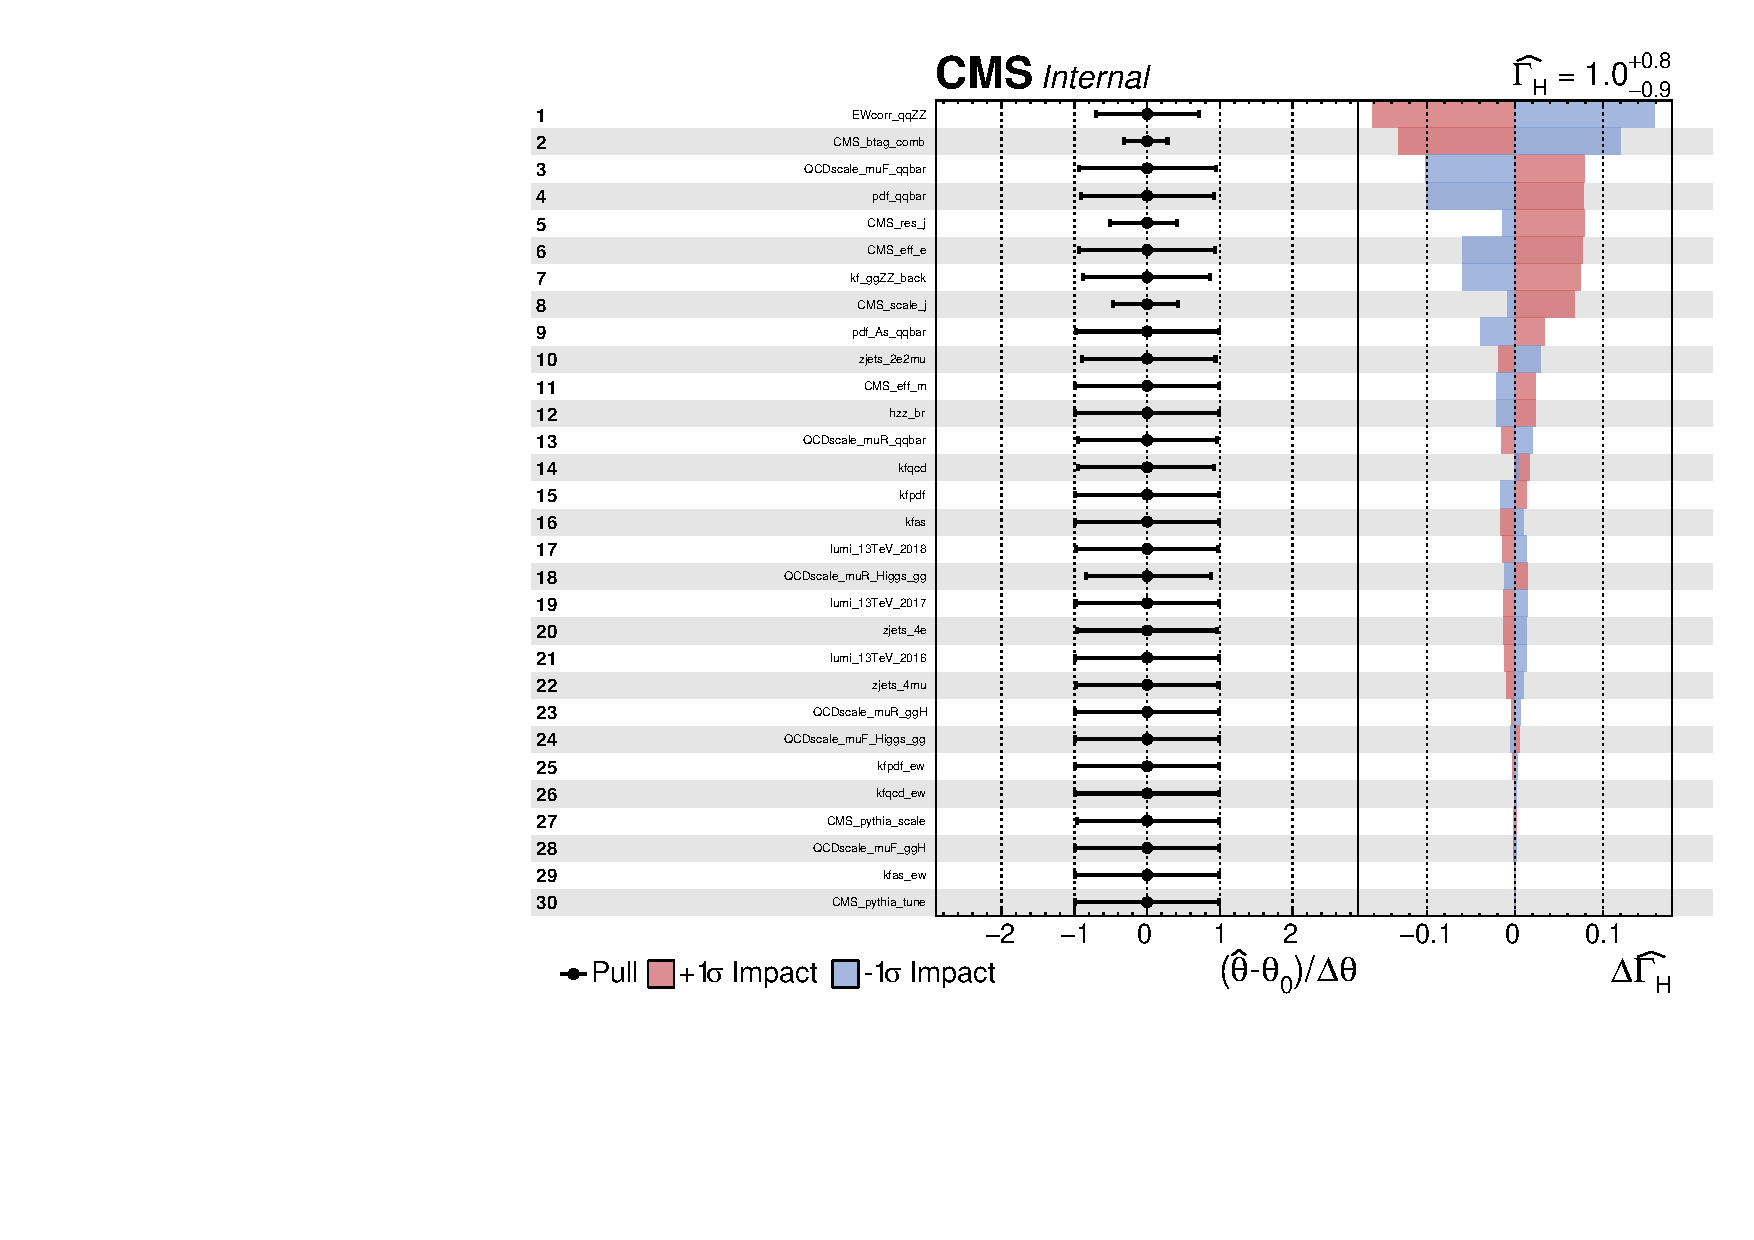
\includegraphics[width=0.85\textwidth]{figures/impacts_all.pdf}
\caption
{
Expected impact of nuisance parameters on the Higgs boson width ratio to the SM value.
\label{fig:impact}
}
\end{center}
\end{figure}

\section{Measurement of Higgs boson properties} \label{sec:results}

\subsection{Higgs boson Width} \label{sec:offshellwidth}

% We perform an extended binned maximum likelihood fit to the on- and off-shell events split in several categories. The final measurements of $m_H$, $\Gamma_H$, and $\mu_{j}$ are conducted using the CMS statistical analysis tool COMBINE~\cite{CMS:2024onh}. 

% The extended likelihood function is constructed using the probability densities in Equations~(\ref{eq:ponshell}) and~(\ref{eq:poffshell}), with each event characterized by the discrete category $k$ and typically three observables $\vec{x}$. The likelihood $\mathcal{L}$ is maximized with respect to the nuisance parameters $\vec{\xi}_{jk}$ describing the systematic uncertainties and the signal strength parameter $\mu$ (total signal strength), or $\mu_F$ (signal strength for ggH) and $\mu_V$ (signal strength for the EW processes). The allowed 68 and 95\% CL intervals are defined using the profile likelihood function, $-2\Delta\ln\mathcal{L} = 1.00$ and $3.84$, respectively, for which exact coverage is expected in the asymptotic limit~\cite{Wilks:1938dza}.

% Constraints on $\Gamma_H$ are set by simultaneously fitting $H\to ZZ\to4\ell$ events from the on- and off-shell regions. The on-shell region corresponds to Scheme 2 in Ref.~\cite{CMS:2021nnc}, where six mutually exclusive event categories are defined and anomalous interactions are constrained to zero. It determines two signal strengths, $\mu_j$ in Equations~(\ref{eq:ponshell}) and~(\ref{eq:poffshell}), 
% labeled as $\mu^\text{on-shell}_{F}$ and $\mu^\text{on-shell}_{V}$, which correspond to production mechanisms driven by fermion and vector boson couplings ofthe \Hboson, respectively. 
% The \Hboson mass is constrained to $m_H$=125.38 GeV \cite{Sirunyan:2020xwk} in this fit. 
% The observed and expected constraints on the \Hboson width are shown in Table~\ref{table:widthoffshellcomb}.
% The likelihood scan of $\Gamma_H$ using the asymptotic approximation method is shown in Figure~\ref{fig:widthscan}. 
% This measurement excludes the scenario of no off-shell \Hboson production with a CL corresponding 
% to 3.0 standard deviations (average expected 1.4).

An extended binned maximum likelihood fit is performed on the combined \onshell and \offshell event samples, divided into multiple analysis categories. The final measurements of $m_H$, $\Gamma_H$, and the signal strength parameters $\mu_{j}$ are carried out using the CMS statistical analysis tool COMBINE~\cite{CMS:2024onh}.

The extended likelihood function is constructed from the probability densities defined in Equations~(\ref{eq:ponshell}) and~(\ref{eq:poffshell}), where each event is characterized by a discrete category index $k$ and typically three observables $\vec{x}$. The likelihood $\mathcal{L}$ is maximized with respect to the nuisance parameters $\vec{\xi}_{jk}$, which encode systematic uncertainties, and the signal strength parameter $\mu$ (representing the total signal yield), or alternatively $\mu_F$ and $\mu_V$, corresponding to the gluon-fusion and electroweak production processes, respectively. Confidence intervals at 68\% and 95\% CL are determined using the profile likelihood method, with thresholds of $-2\Delta\ln\mathcal{L} = 1.00$ and $3.84$ ~\cite{Wilks:1938dza}.
% Confidence intervals at 68\% and 95\% CL are determined using the profile likelihood method, with thresholds of $-2\Delta\ln\mathcal{L} = 1.00$ and $3.84$, respectively, consistent with asymptotic coverage expectations~\cite{Wilks:1938dza}.

Constraints on $\Gamma_H$ are extracted from a simultaneous fit to $H \to ZZ \to 4\ell$ events in both the \onshell and \offshell regions. The \onshell region follows Scheme 2 as defined in Ref.~\cite{CMS:2021nnc}, where six mutually exclusive categories are used and anomalous Higgs interactions are set to zero. This fit yields two signal strength parameters, $\mu^\text{on-shell}_{F}$ and $\mu^\text{on-shell}_{V}$, as defined in Equations~(\ref{eq:ponshell}) and~(\ref{eq:poffshell}), corresponding to production via fermionic and vector boson couplings of the \Hboson, respectively. The Higgs boson mass is fixed to $m_H = 125.38$\,GeV~\cite{Sirunyan:2020xwk}.

The observed and expected constraints on the Higgs boson width are presented in Table~\ref{table:widthoffshellcomb}, while the likelihood scan of $\Gamma_H$, obtained using the asymptotic approximation, is shown in Figure~\ref{fig:widthscan}. This measurement excludes the hypothesis of no off-shell Higgs boson production with a CL corresponding to 3.0 standard deviations (compared to an average expected 1.4).

The results of this analysis with the SM-like couplings are also combined with the prior CMS \offshell $H\to ZZ\to2\ell2\nu$ analysis~\cite{CMS:2022ley}, giving the first CMS measurement of $\Gamma_H$ using the full $4\ell$ and $2\ell2\nu$ data sample collected during Run 2. 
The observed and expected $\Gamma_H$ measurements are shown in Table~\ref{table:widthoffshellcomb} and Figure~\ref{fig:widthscan} and supersede the previous CMS results~\cite{CMS:2022ley} under the SM-like coupling assumption. These combined fit results rule out the scenario of no \offshell \Hboson production
with a CL corresponding to 3.8 standard deviations (average expected 2.4).

\begin{table*}[!htb]
    \centering
    % \renewcommand{\arraystretch}{1.25}
    \begin{tabular}{lll}
        Channel     & Observed $\Gamma_H$ (MeV)        &  Expected $\Gamma_H$ (MeV)  \\
        \hline
        $4\ell$ on- and off-shell    & $2.9^{+2.3}_{-1.7} \ [0.3,7.9]$ & $4.1\pm 4.0 \ [<11.5 ]$ \\
        $4\ell$ on- and off-shell  + $2\ell2\nu$ off-shell  & $3.0^{+ 2.0 }_{- 1.5 }  \ [0.6, 7.3]$ & $4.1\pm3.5 \ [0.1,10.5]$ \\
    \end{tabular}
    \caption{Summary of the total Higgs boson width $\Gamma_H$ measurement, showing the 68\%~CL (central values with uncertainties)
    and 95\%~CL (in square brackets) intervals for the $H \to ZZ \to 4 \ell$ channel alone and in combination with the off-shell $H \to ZZ \to 2 \ell 2 \nu$ channel~\cite{PhysRevD.111.092014}.}
    \label{table:widthoffshellcomb}
\end{table*}

\begin{figure}[!htb]
    \centering
    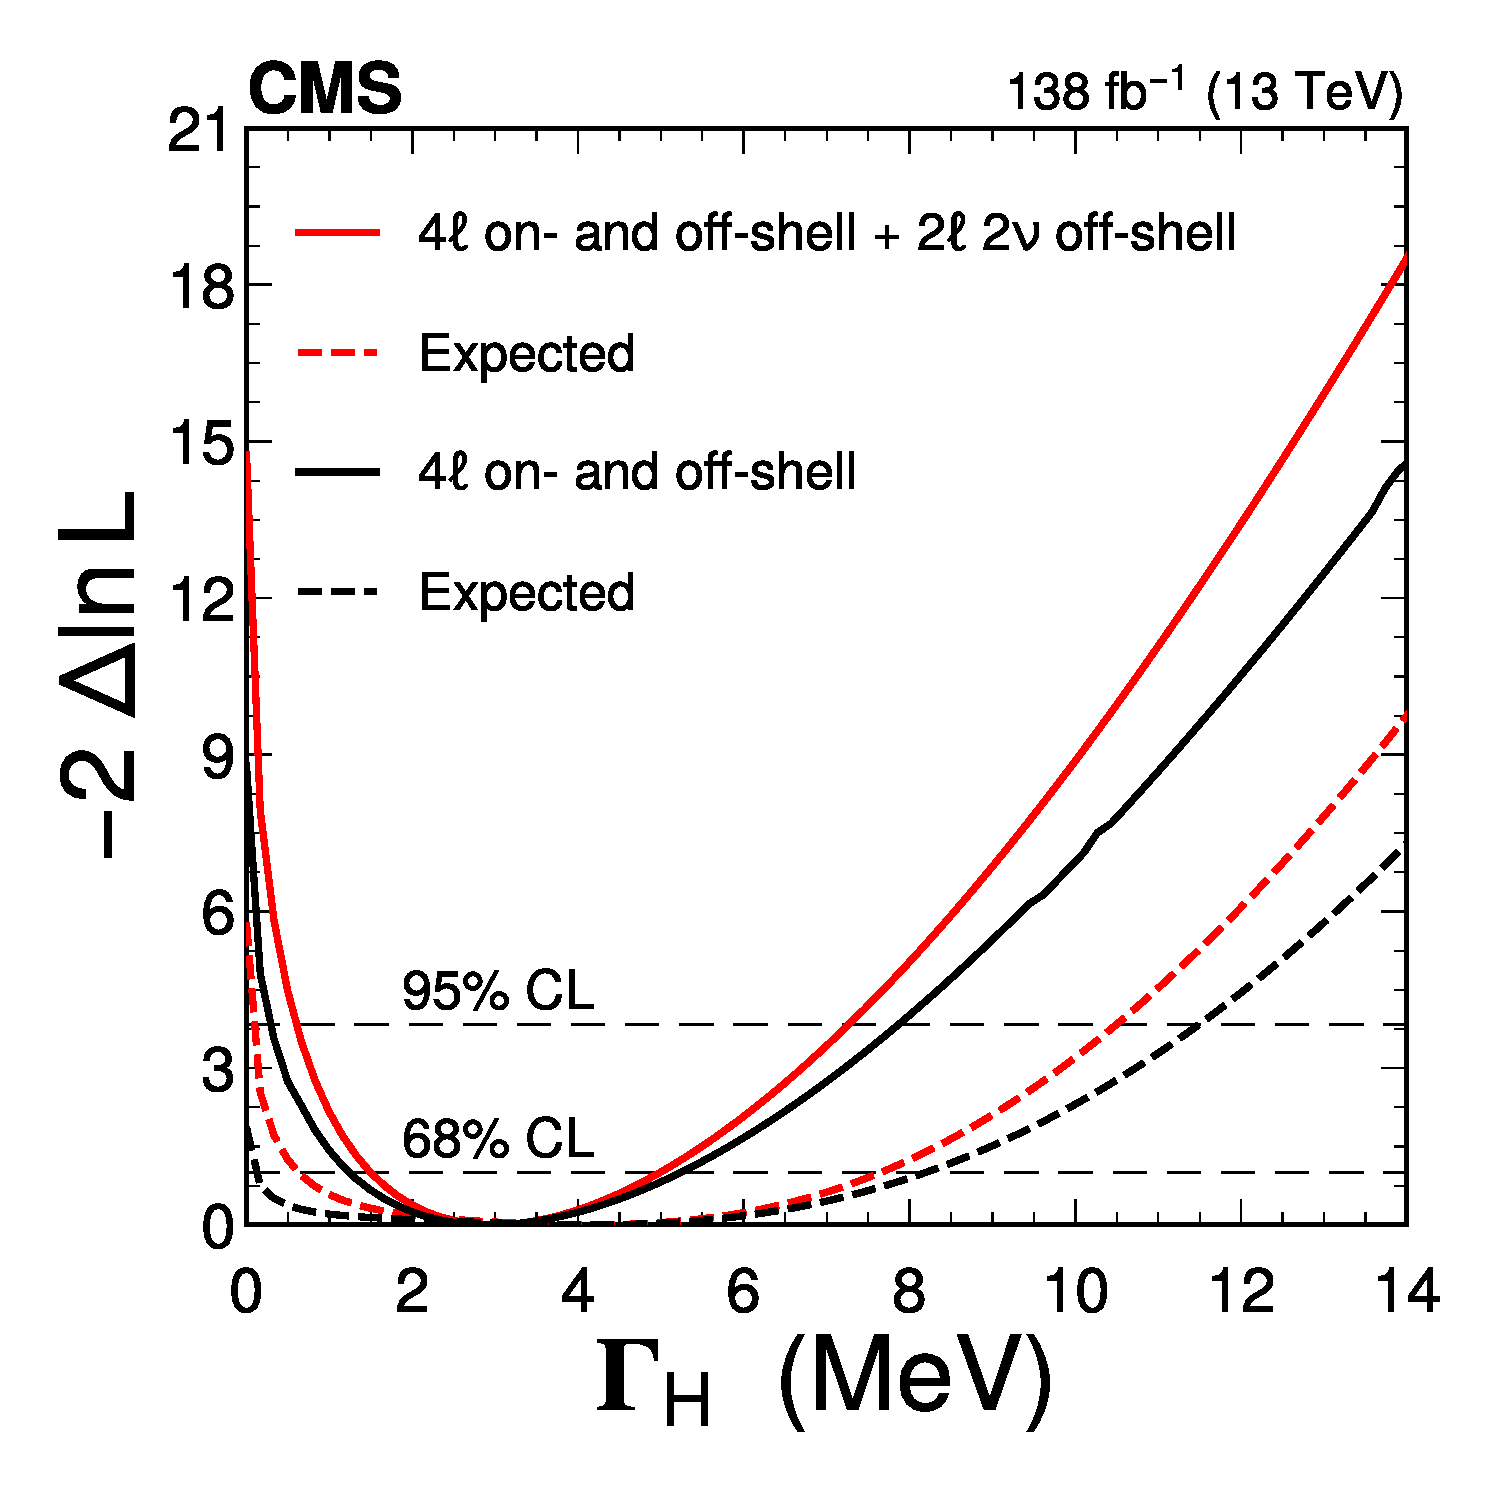
\includegraphics[width=0.8\textwidth]{Figure_011.pdf}  
    \caption{
        Observed (solid) and expected (dashed) profile likelihood projections from the \Hboson width fit using on- and off-shell production from this analysis. The analysis of the off-shell $H\to ZZ\to4\ell$ channel combined with the on-shell $H\to ZZ\to4\ell$ channel~\cite{CMS:2021nnc} is shown in black. The full combination of $H\to ZZ\to4\ell$ with the off-shell $H\to ZZ\to2\ell2\nu$~\cite{CMS:2022ley} is given in red. The black horizontal dashed lines show the 68 and 95\% CL values~\cite{PhysRevD.111.092014}.}
    \label{fig:widthscan} 
\end{figure}

% The observed limits on $\Gamma_H$ are stronger than the average expected values from simulation. 
% This is supported by our template plots, specifically the upper left plot of Figure~\ref{fig:ObservablesCat}, where the number of observed events in the sensitive region of $m_{4\ell}>340$ GeV and $\Dbkg > 0.6$ in the Untagged category is below the expected value (but still consistent). 

% The smaller number of events in this region favors the hypothesis of negative interference between the signal and background contributions, which dominates over the pure signal contributions for $\Gamma_H$ values near the SM value. Therefore, large and very small values of $\Gamma_H$ are disfavored.

The observed limits on $\Gamma_H$ are more stringent than the average expectations derived from simulation. This behavior is supported by the template distributions, in particular the upper-left panel of Figure~\ref{fig:ObservablesCat}, where the number of observed events in the region defined by $m_{4\ell} > 340$\,GeV and $\Dbkg > 0.6$ in the Untagged category is lower than expected, though still statistically consistent.

A reduced number of events in this sensitive region favors the hypothesis of greater negative interference between the signal and background contributions, which becomes dominant over the pure signal contributions for $\Gamma_H$ values near the SM value. As a result, both large and very small values of $\Gamma_H$ are disfavored by the data.

\subsection{Off-shell Signal Strength}

% The \offshell region fit can also be performed without relating its signal strength to that for the \onshell region.
% In this case, the signal strength is modified by the parameter $\mu^\text{off-shell}$ common to all production 
% mechanisms, with $\Gamma_H=\Gamma_H^{SM}$ in Eq.~(\ref{eq:poffshell}), and the SM expectation corresponding to $\mu^\text{off-shell}=1$. 
% In addition, we also perform a fit of the \offshell events with two unconstrained parameters $\mu^\text{off-shell}_{F}$ and
% $\mu^\text{off-shell}_{V}$, which express the signal strengths in the ggH and EW processes, respectively.
% The measured signal strengths are reported in Table~\ref{table:muoffshell} and a 2D scan of these parameters 
% is presented in Figure~\ref{fig:muoffshell}. The observed limits on signal strength in the \offshell region are stronger than expected on average, following a trend similar to that previously discussed for $\Gamma_H$.

An alternative approach to the \offshell region fit involves decoupling its signal strength from that of the \onshell region. In this configuration, the signal yield is scaled by a single parameter, $\mu^\text{off-shell}$, which is common to all production mechanisms. The total Higgs boson width is fixed to its SM value, $\Gamma_H = \Gamma_H^{\mathrm{SM}}$, in Eq.~(\ref{eq:poffshell}), and the SM expectation corresponds to $\mu^\text{off-shell} = 1$.

In addition, a more general fit is performed with two unconstrained signal strength parameters: $\mu^\text{off-shell}_{F}$ and $\mu^\text{off-shell}_{V}$, corresponding to gluon-fusion and electroweak production mechanisms, respectively. The measured values of these parameters are reported in Table~\ref{table:muoffshell}, and their joint CL regions are shown in the two-dimensional likelihood scan in Figure~\ref{fig:muoffshell}. The observed constraints on the \offshell signal strengths are stronger than the average expected values, consistent with the trend observed earlier in the $\Gamma_H$ analysis.

\begin{table*}[!htb]
\centering
% \renewcommand{\arraystretch}{1.6}
\begin{tabular}{lcc}
  Parameter                & {Observed}          &  {Expected}   \\
  \hline
  $\mu^\text{off-shell}$ &  $0.67^{+ 0.42}_{-0.32 }\ [0.14,1.54]$ & $1.00^{+ 0.83}_{-0.84}\ [0.02,2.46]$ \\
  $\mu_F^\text{off-shell}$ &  $0.57^{+ 0.50}_{- 0.36}\ [0.04,1.61]$ & $1.00^{+0.90}_{-0.98}\ [{<}2.62]$\\
  $\mu_V^\text{off-shell}$ &  $ 0.87^{+0.93}_{-0.57}\ [0.05,2.90]$ & $1.00^{+1.95}_{-0.89}\ [{<}4.34]$ \\
\end{tabular}
\caption{
  Measured values of the signal strengths $\mu^\text{off-shell}$, $\mu_F^\text{off-shell}$, and $\mu_V^\text{off-shell}$,
  and their 68\% and 95\% (in square brackets) CL intervals from the combined fit to the \offshell $H\to ZZ\to4\ell$ and $2\ell2\nu$ channels.
}
\label{table:muoffshell}
\end{table*}

\begin{figure}[!htb]
  \centering
  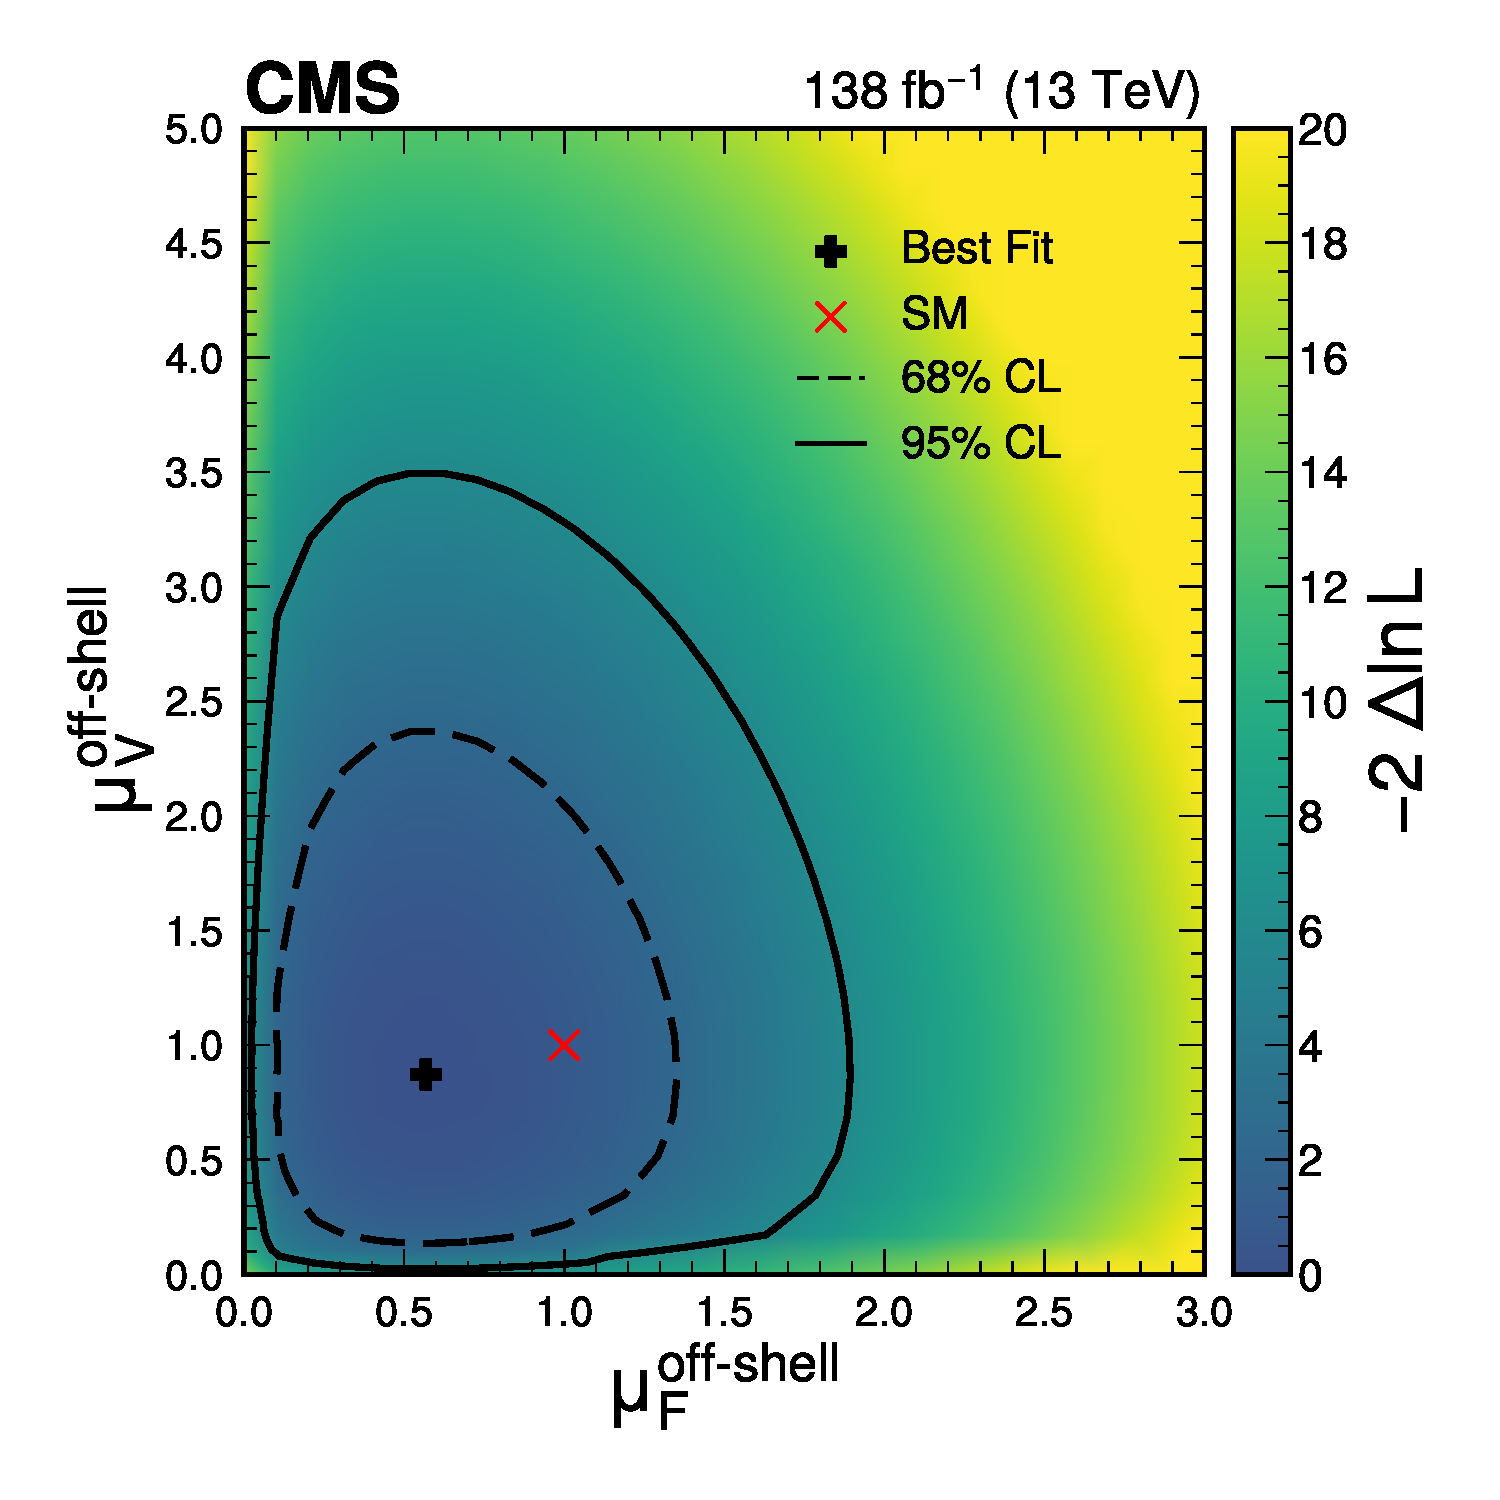
\includegraphics[width=0.8\textwidth]{figures/Figure_012.pdf}  
  \caption
      {
        Observed 2D profile likelihood projection of the \offshell signal strength parameters ($\mu^\text{off-shell}_{F}$, $\mu^\text{off-shell}_{V}$) 
        from the fit to the combined \offshell $H\to ZZ\to4\ell$ and $2\ell2\nu$ channels. The best fit value is shown by the black cross and the SM 
        prediction by the red x. The 68 and 95\% CL contours are given by the dashed and solid curves, respectively. The color scale to the right of the plot relates the quantitative values~\cite{PhysRevD.111.092014}.
      }
    \label{fig:muoffshell} 
\end{figure}

\subsection{Kappa Framework}

% The above $\Gamma_H$ constraints assume the expected SM-like evolution of the \Hboson couplings over a large $m_{4\ell}$ range.
% The anomalous contributions to the $H{VV}$ vertex in EW production and \Hboson decay were evaluated in our earlier analyses 
% using a smaller data set~\cite{Sirunyan:2019twz,CMS:2022ley}, and the constraints on $\Gamma_H$ remained consistent.
% However, the predominance of the top quark in the ggH loop is assumed here and in our previous analyses. 
% If there are additional contributions, such as from yet undiscovered heavy particles, then the $m_{4\ell}$ evolution 
% in the \offshell region would be altered.

% To investigate the impact of large-mass yet undiscovered particles in the ggH loop,
% we introduce a new heavy quark $Q$ with an unconstrained coupling strength 
% $\kappa_{Q}$ in the likelihood parametrization, as described in Refs.~\cite{Gritsan:2020pib,Davis:2021tiv}.
% In the framework of effective field theories, the contribution of $Q$ can be interpreted 
% as a point-like interaction that encapsulates the influence of any heavy particles present in the loop.
% The parameterization in Equation~(\ref{eq:poffshell}) is extended to include the templates for terms proportional to 
% $\kappa^2_{Q}$ and $\kappa_{Q}$, utilizing simulations reweighted with the MELA package
% in the limit of the infinite $Q$ mass. 
% The $m_{4\Pell}$ shape in the \offshell region shows contrasting patterns between the SM ggH production, 
% which is mainly affected by the top quark loop with the $2m_{t}$ threshold effect, 
% and the \Hboson produced via ggH loop involving the heavy quark $Q$~\cite{Gritsan:2020pib}.

% An unconstrained $\kappa_{Q}$ introduces additional uncertainty into the $m_{4\ell}$ 
% dependence in the \offshell region, resulting in less stringent limits on $\Gamma_H$.
% However, both on- and \offshell $H\to4\ell$ data constrain the possible values of $\kappa_{Q}$, 
% and the constraints on $\Gamma_H$ remain largely consistent with those for $\kappa_{Q}=0$.
% The resulting $\Gamma_H$ measurement from the combined on- and \offshell events is $2.7^{+2.7}_{-1.8}$ MeV 
% (expected $4.1^{+5.5}_{-4.1}$ MeV). 
% The observed (expected) 95\%\, \CL interval is $\,[0.1,8.8]\, (\,[{<}14.4]\,)$ MeV.
% We note that combining measurements from other \onshell \Hboson production and decay channels 
% in the future will lead to much stricter constraints on $\kappa_{Q}$, reducing the flexibility 
% to alter the SM-like evolution of the \Hboson couplings over a large $m_{4\ell}$ range.

The $\Gamma_H$ constraints presented in Section~\ref{sec:offshellwidth} assume SM-like evolution of the Higgs boson couplings across a wide $m_{4\ell}$ range. Anomalous contributions to the $HVV$ vertex in EW production and Higgs boson decay were investigated in earlier analyses using smaller datasets~\cite{Sirunyan:2019twz,CMS:2022ley}, and the resulting $\Gamma_H$ constraints remained consistent. However, both the current and previous analyses assume that the gluon-fusion production mechanism is dominated by the top quark loop. If additional heavy particles contribute to the loop, this assumption would no longer hold, and the $m_{4\ell}$ dependence in the \offshell region could be significantly modified.

To explore the impact of potential contributions from new heavy particles in the $gg \to H$ loop, a hypothetical heavy quark $Q$ is introduced with an unconstrained coupling strength $\kappa_Q$, such as is described in Section~\ref{sec:kappa}~\cite{Gritsan:2020pib,Davis:2021tiv}. In the framework of effective field theory, the influence of such a particle is modeled as a point-like interaction that encapsulates its loop effects. The parametrization in Equation~(\ref{eq:poffshell}) is extended to include template components proportional to $\kappa_Q$ and $\kappa_Q^2$, obtained from simulations reweighted using the MELA package in the limit of infinite $Q$ mass. 

The $m_{4\ell}$ distribution in the \offshell region exhibits different behaviors for SM-like gluon fusion—dominated by the top quark with the $2m_t$ threshold—and for scenarios involving the additional heavy quark $Q$~\cite{Gritsan:2020pib}. Allowing $\kappa_Q$ to vary freely introduces additional uncertainty in the $m_{4\ell}$ spectrum, which weakens the sensitivity to $\Gamma_H$. Nonetheless, both the \onshell and \offshell $H \to 4\ell$ data constrain the allowed values of $\kappa_Q$, and the resulting $\Gamma_H$ constraints remain broadly consistent with the $\kappa_Q = 0$ case.

From the simultaneous fit to the \onshell and \offshell regions, the observed width is measured to be $\Gamma_H = 2.7^{+2.7}_{-1.8}$\,MeV, with an expected value of $4.1^{+5.5}_{-4.1}$\,MeV. The observed (expected) 95\% confidence interval is $[0.1,\,8.8]$\,MeV ($[\,{<}14.4]$\,MeV). Future combinations with measurements from other \onshell Higgs boson production and decay channels are expected to significantly improve constraints on $\kappa_Q$, thereby reducing the allowed deviations from SM-like coupling evolution across the high-$m_{4\ell}$ regime.

\subsection{Other measurements}

\subsubsection{On-shell Mass}

As mentioned previously in Section~\ref{sec:onshell}, compared to the previous CMS on-shell \Hboson measurements in this channel~\cite{Sirunyan:2017exp}, the statistical and systematic uncertainties affecting $m_{H}$ have been reduced by our collaborators' inclusion of the beam spot in a refit of the muon tracks; adoption of an improved event categorization procedure; and detailed study of the lepton momentum scale and resolution~\cite{PhysRevD.111.092014}.

% The \Hboson mass is measured, using on-shell production, by fitting the $m_{4\ell}$ distribution in the mass range $105< m_{4\ell} < 140$ GeV, using different likelihood models.
% The results have been determined using the CMS statistical analysis tool COMBINE~\cite{CMS:2024onh}, 
% which is based on the \textsc{RooFit}~\cite{Verkerke:2003ir} and \textsc{RooStats}~\cite{Moneta:2010pm} frameworks.\\

% Table~\ref{table:Mass1Dresults} shows the mass measurements obtained from the 1D approach, where no further assumptions have been made. In comparison to the 1D model, the 1D$^{'}_\text{BS}$ model reduces the uncertainty by about 15\%. Implementing the $\delta m_{4\ell} / m_{4\ell}$ categorization then gives the $\mathcal{N}$--1D$'_\text{BS}$ model, which leads to an additional 10\% improvement. 
% Finally, using the \Dkinbkg discriminant to reduce the background produces the $\mathcal{N}$--2D$'_\text{BS}$ model with another 4\% improvement.  

Table~\ref{table:Mass_results} shows the resulting $m_{4\ell}$ measurements from our collaborators' complete procedure. All the measured $m_{4\ell}$ values from the different fits are statistically compatible, given their uncertainties and correlations. Figure~\ref{MassLikelihoodScan} displays the observed 1D likelihood scans as functions of $m_H$, from the fits for the different $4\ell$ categories and combined.

Combining all the $m_{4\ell}$ final states and data-taking years, our final result is 
$m_H = 125.04~\pm~0.11$ (stat)$~\pm~0.05$ (syst) = $125.04~\pm~0.12$ GeV.
The largest systematic uncertainty is from the lepton momentum scale and equals 0.03 and 0.04 GeV for final states with muons and electrons, respectively.

% \begin{table*}[!htb]	
%   \centering
%   \topcaption{
%     Best fit values for the mass of the \Hboson measured in the inclusive 4$\ell$ final state and separately for different flavor categories using the 1D approach.
%     Uncertainties are separated into statistical and systematic uncertainties.
%     Expected uncertainties are also given assuming $m_{H} = 125.38$ GeV \cite{Sirunyan:2020xwk}.
%   }
%   \renewcommand{\arraystretch}{1.6}
%     \begin{tabular}{lcc}
%       $4\ell$ category & Observed ($\pm$stat$\pm$syst) (GeV) & Expected uncertainty ($\pm$stat$\pm$syst)  (GeV) \\
%       \hline
%       Inclusive &	$124.98 \pm 0.14 \pm0.05$ & $ \pm 0.14 \pm 0.05$ \\
%       $4\mu$ &	$124.87 \pm 0.17\pm0.04$ & $\pm 0.18 \pm 0.04$ \\
%       $2\mu2e$ &	$125.32^{+0.36}_{-0.37}\pm0.10$ & $^{+0.34+0.09}_{-0.34-0.10}$ \\
%       $2e2\mu$ &        $125.23^{+0.36+0.09}_{-0.35-0.11}$ & $^{+0.35+0.09}_{-0.35-0.10}$ \\
%       ${4e}$ &    $124.94^{+0.68}_{-0.71} \pm 0.20$ & $^{+0.51+0.18}_{-0.51-0.20}$ \\
%   \end{tabular}
%   \label{table:Mass1Dresults}
% \end{table*}

\begin{table*}[!htb]	
  \centering
  % \renewcommand{\arraystretch}{1.6}
    \begin{tabular}{lccc}
      $4\ell$ category & Observed ($\pm$stat$\pm$syst) (GeV) & Expected uncertainty ($\pm$stat$\pm$syst) (GeV)  \\
      \hline
      Inclusive  & $125.04\pm0.11 \pm 0.05$	&	 $\pm 0.11\pm  0.05$ \\
      $4\mu$ & $124.90 \pm 0.14 \pm 0.05$	&	$\pm 0.14\pm  0.04$ \\
      $2e2\mu$ &        $125.50^{+0.25}_{-0.24}\pm0.10$      &       $\pm0.24\pm0.10$ \\
      $2\mu2e$ &        $125.20^{+0.27+0.11}_{-0.26-0.07}$     &        $\pm0.27\pm0.10$ \\
      $4e$ &	$124.70^{+0.49}_{-0.47}\pm0.20$     &	$\pm0.38\pm0.20$ \\ 
  \end{tabular}
  \caption{Best fit values for the mass of the \Hboson measured in the inclusive 4$\ell$ final state and separately for different flavor categories, using the final fit configuration~\cite{PhysRevD.111.092014}. Uncertainties are separated into statistical and systematic uncertainties. Expected uncertainties are also given assuming $m_{H} = 125.38$ GeV~\cite{Sirunyan:2020xwk}.}
  \label{table:Mass_results}
\end{table*}

\begin{figure}[!htb]
  \centering
  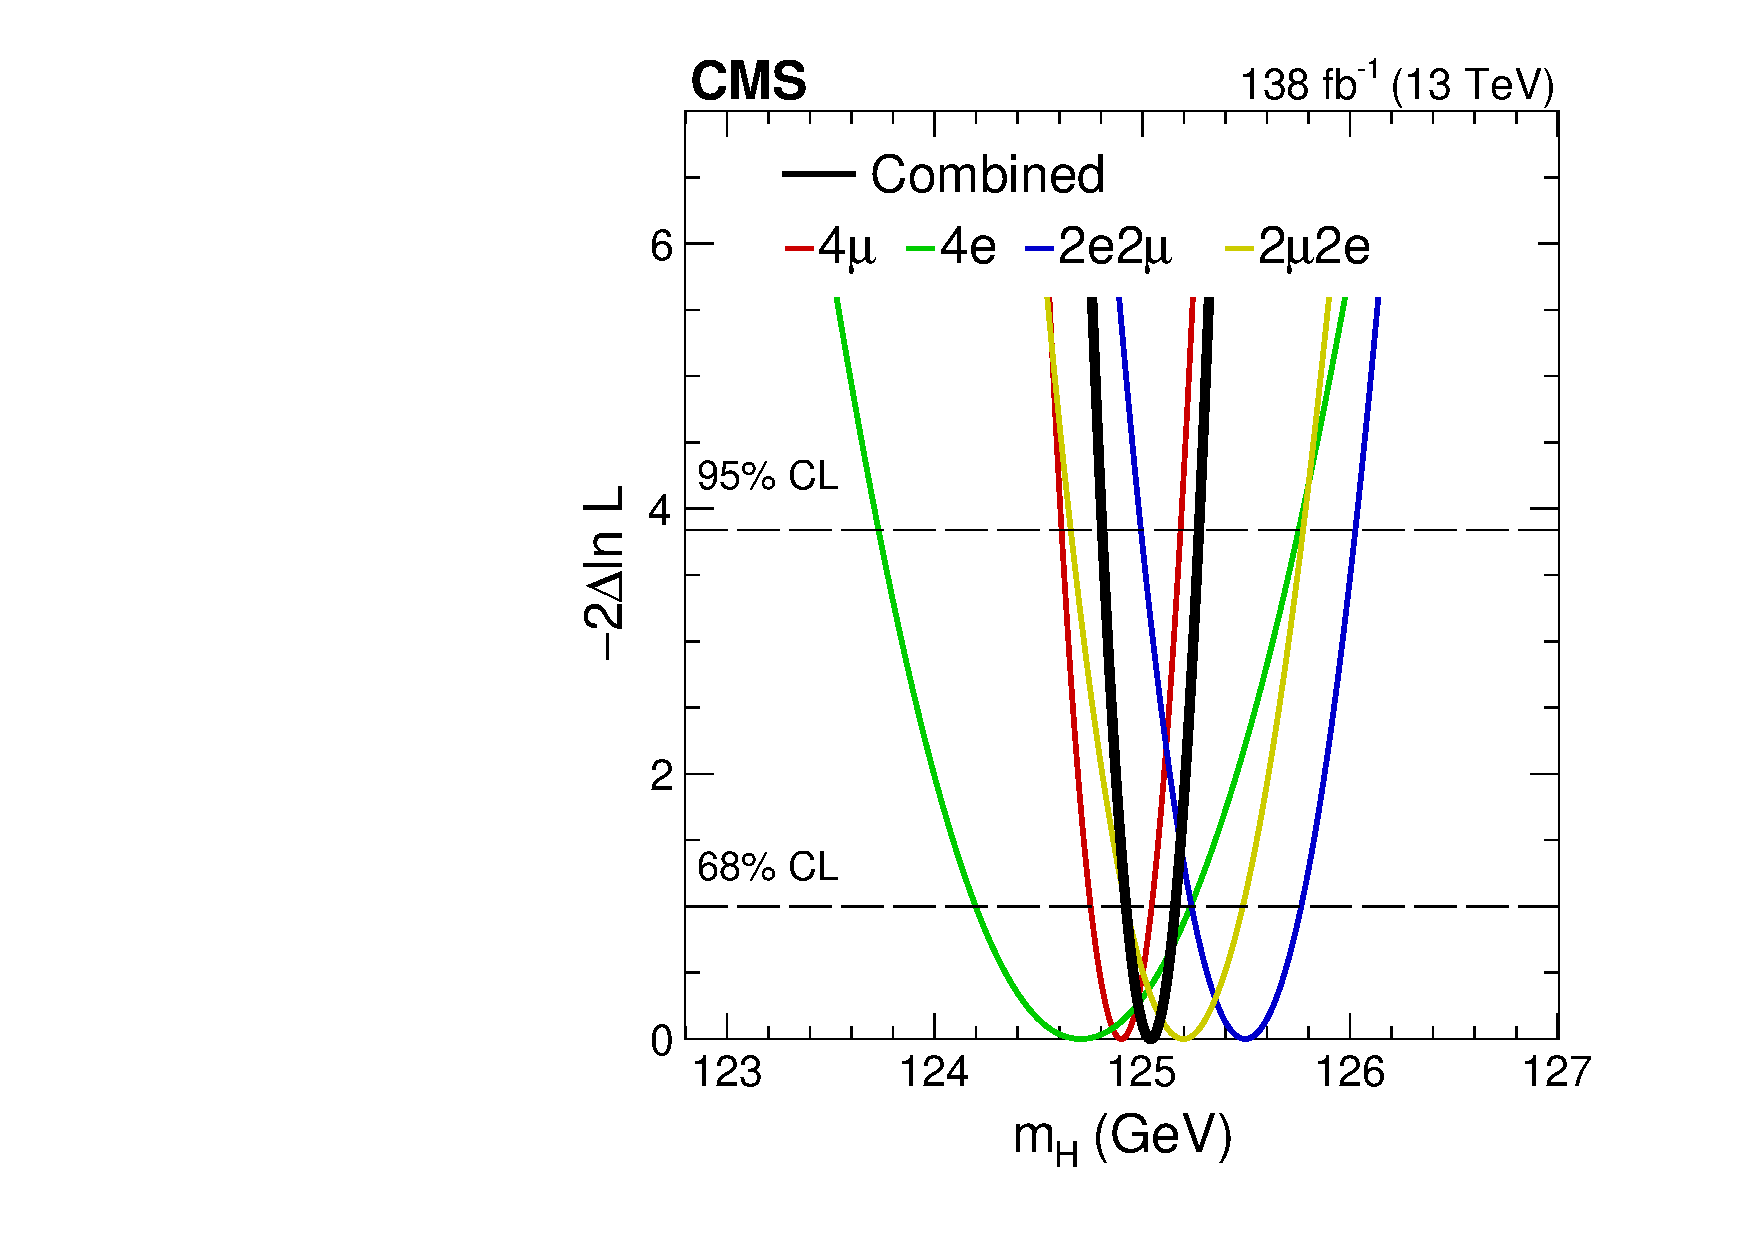
\includegraphics[width=0.8\textwidth]{Figure_008.pdf}
  \caption{The profile likelihood from the $m_H$ fit using the comprehensive on-shell model for each of the 4$\ell$ categories and combined.  The change in likelihood corresponding to 68 and 95\% CLs are shown by the dashed horizontal lines. Both statistical and systematic uncertainties are included in the fits~\cite{PhysRevD.111.092014}.}
  \label{MassLikelihoodScan}
\end{figure}

% As a check on the analysis technique and the systematic uncertainty from this method, the 
% 1D$^{'}_\text{BS}$ model is applied to $Z \to 4\ell$ events in the $m_{4\ell}$ range 70--105  GeV. The signal shape is obtained using a convolution of a Breit--Wigner function and a double-sided Crystal Ball function.
% The fitted values of $m_Z$ in different subchannels are $m_Z^{4\mu} = 91.02 \pm 0.14$ GeV, $m_Z^{4e} = 91.18 \pm 0.45$ GeV, $m_Z^{2e2\mu} = 91.40 \pm 0.29$ GeV, and $m_Z^{2\mu2e} = 91.40 \pm 0.37$ GeV, leading to a combined value of $m_Z = 91.17 \pm 0.12$ GeV, consistent with the world-average Z boson mass~\cite{Agashe:2014kda} and with the uncertainty in agreement with the expected value of $\pm~0.12$ GeV from simulation.

The results from this analysis are combined with those extracted using data recorded with the  
CMS detector during Run 1 at $\sqrt{s}= 7$ and 8 TeV~\cite{Chatrchyan:2013mxa}. 
Since this analysis uses an improved method to extract the systematic uncertainties affecting lepton momentum, 
the lepton energy scales and resolution uncertainties are considered uncorrelated between the two runs. The combined observed result from both data-taking periods is $m_H$ = 125.08 $\pm$ 0.12 GeV = 125.08 $\pm$ 0.10\stat $\pm$ 0.05\syst GeV. The corresponding expected statistical and systematic uncertainties are $\pm$0.10 and $\pm$0.05 GeV, respectively. Figure~\ref{Run1Run2_scan} presents a summary of the \Hboson mass measurements by the CMS Collaboration in the four-lepton decay channel.

\begin{figure*}[!htb]
  \centering
  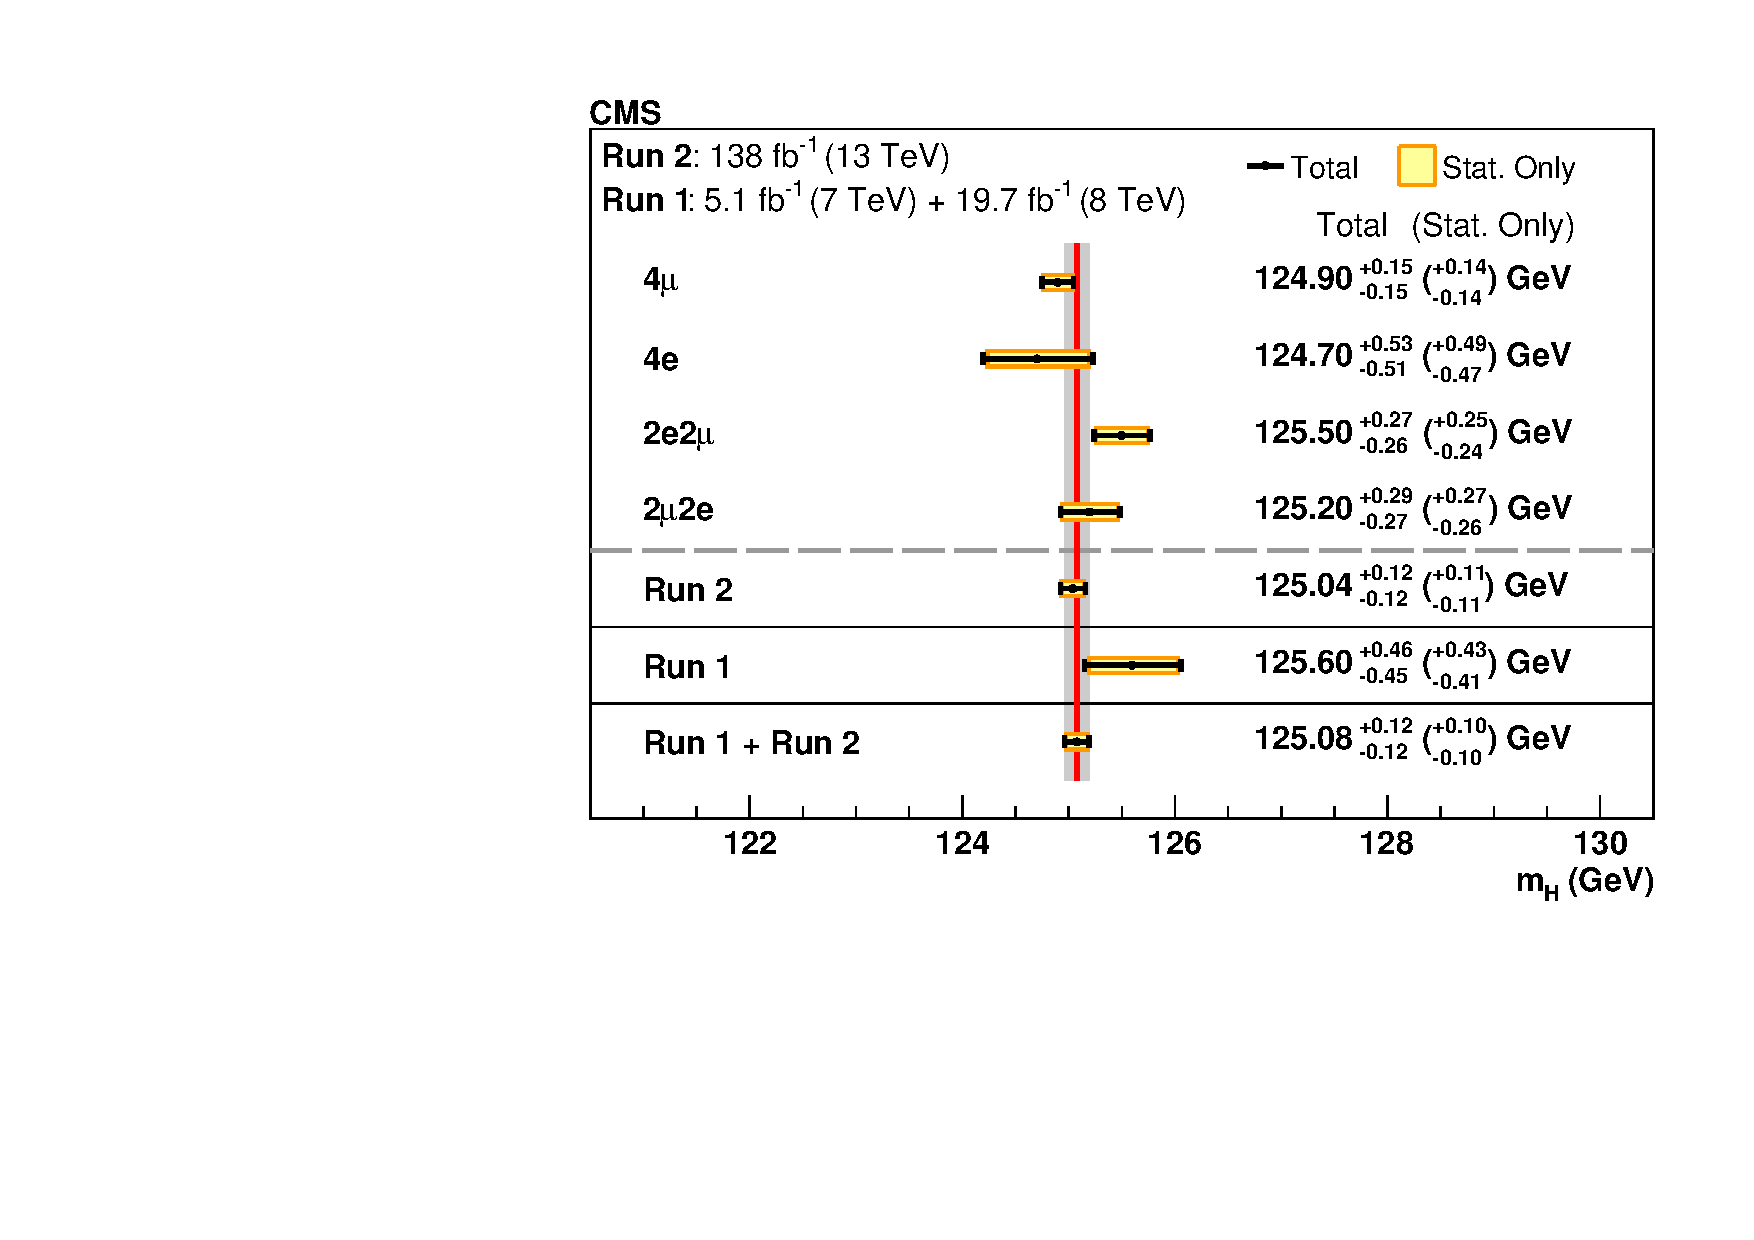
\includegraphics[width=0.8\textwidth]{Figure_009.pdf}
  \caption{Summary of the CMS Higgs boson mass measurements using the four-lepton final state. The red vertical line and the gray column represent the best fit value and the total uncertainty, respectively, as measured by combining Run 1 and Run 2 data. The yellow band and horizontal black bars show the statistical and total uncertainties in each measurement, respectively. The value of each measurement is given, along with the total and statistical only (in parentheses) uncertainties~\cite{PhysRevD.111.092014}.}
  \label{Run1Run2_scan}
\end{figure*}

\subsubsection{On-shell Width}

The final \onshell model is also used for an on-shell-only Higgs boson width measurement, with the signal model extended to include the $\Gamma_H$ parameter. Since the theoretical prediction for $\Gamma_H$ is very close to zero---a strict lower bound---confidence intervals are constructed using the Feldman-Cousins approach~\cite{FC}. The confidence level (CL) was evaluated by our collaborators for various width hypotheses using distributions derived from simulated pseudo-experiments~\cite{PhysRevD.111.092014}.

The observed (expected) upper limit on $\Gamma_H$ is 50\,(320)\,MeV at 68\% CL and 330\,(640)\,MeV at 95\% CL. Although the observed limit is significantly lower than the expected one, both are statistically compatible. The resulting distribution of 1-CL as a function of $\Gamma_H$ is shown in Figure~\ref{OnShell_width}. This measurement is statistically limited; the dominant uncertainty arises from statistical fluctuations, while the leading systematic uncertainty is driven by the lepton momentum resolution.

\begin{figure}[!htb]
  \centering
  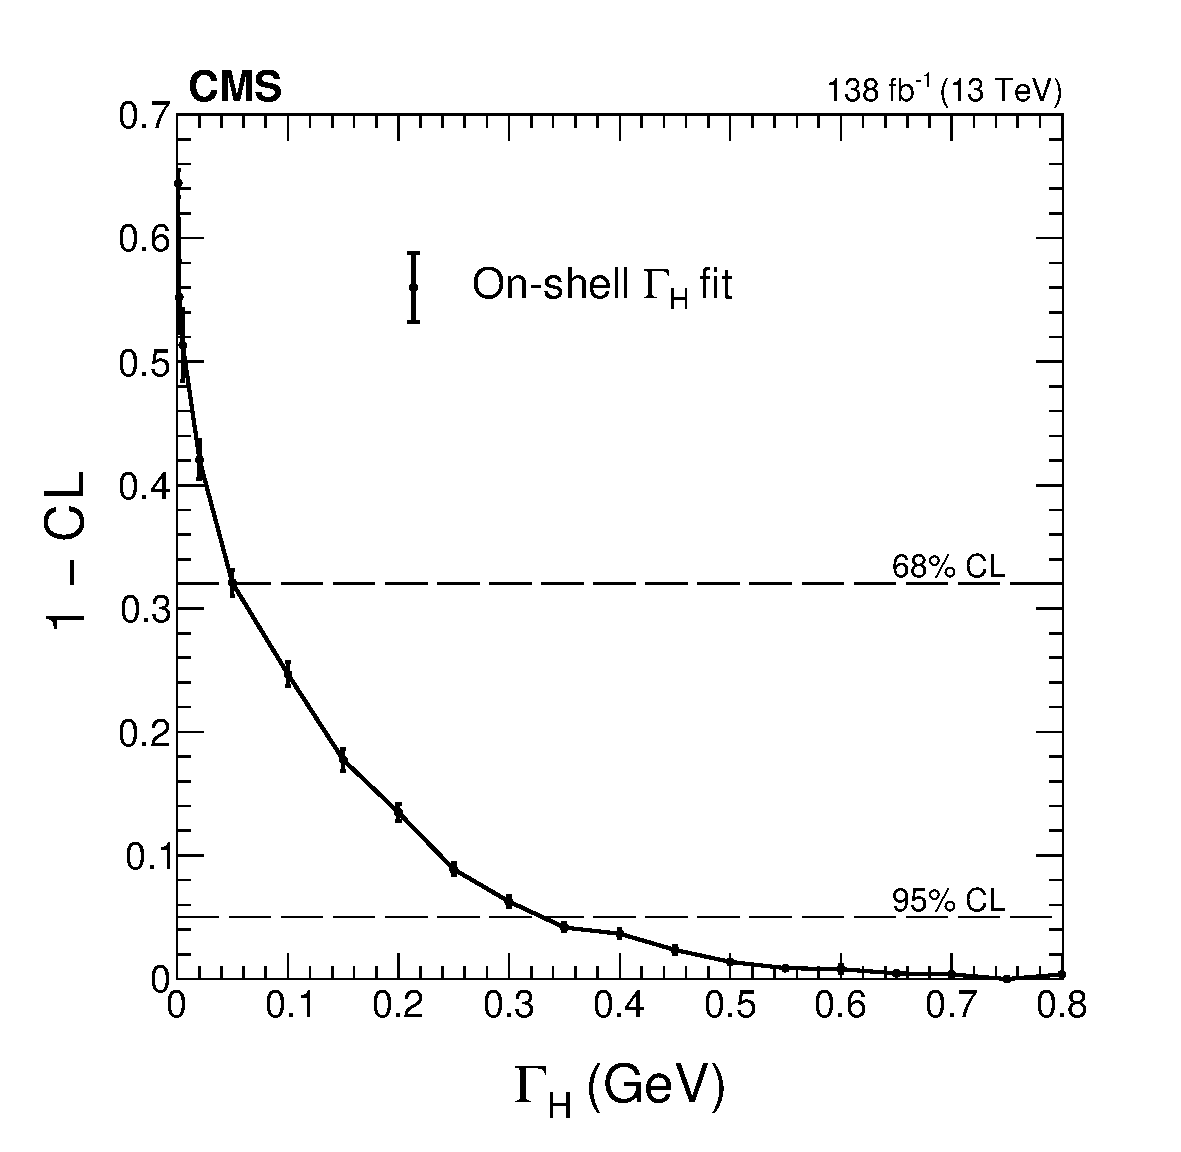
\includegraphics[width=0.8\textwidth]{figures/Figure_010.pdf}
  \caption{Distribution of 1-CL versus $\Gamma_H$ from the fit used to measure the Higgs boson width using on-shell production only. The CL values shown by the points are extracted using the Feldman-Cousins approach. The vertical bars on the points represent the spread in the simulated pseudo-experiment outcomes. The 68\% and 95\% CL thresholds are indicated by the dashed horizontal lines~\cite{PhysRevD.111.092014}.}
  \label{OnShell_width}
\end{figure}
